\documentclass[twoside]{book}

% Packages required by doxygen
\usepackage{fixltx2e}
\usepackage{calc}
\usepackage{doxygen}
\usepackage[export]{adjustbox} % also loads graphicx
\usepackage{graphicx}
\usepackage[utf8]{inputenc}
\usepackage{makeidx}
\usepackage{multicol}
\usepackage{multirow}
\PassOptionsToPackage{warn}{textcomp}
\usepackage{textcomp}
\usepackage[nointegrals]{wasysym}
\usepackage[table]{xcolor}

% Font selection
\usepackage[T1]{fontenc}
\usepackage[scaled=.90]{helvet}
\usepackage{courier}
\usepackage{amssymb}
\usepackage{sectsty}
\renewcommand{\familydefault}{\sfdefault}
\allsectionsfont{%
  \fontseries{bc}\selectfont%
  \color{darkgray}%
}
\renewcommand{\DoxyLabelFont}{%
  \fontseries{bc}\selectfont%
  \color{darkgray}%
}
\newcommand{\+}{\discretionary{\mbox{\scriptsize$\hookleftarrow$}}{}{}}

% Page & text layout
\usepackage{geometry}
\geometry{%
  a4paper,%
  top=2.5cm,%
  bottom=2.5cm,%
  left=2.5cm,%
  right=2.5cm%
}
\tolerance=750
\hfuzz=15pt
\hbadness=750
\setlength{\emergencystretch}{15pt}
\setlength{\parindent}{0cm}
\setlength{\parskip}{3ex plus 2ex minus 2ex}
\makeatletter
\renewcommand{\paragraph}{%
  \@startsection{paragraph}{4}{0ex}{-1.0ex}{1.0ex}{%
    \normalfont\normalsize\bfseries\SS@parafont%
  }%
}
\renewcommand{\subparagraph}{%
  \@startsection{subparagraph}{5}{0ex}{-1.0ex}{1.0ex}{%
    \normalfont\normalsize\bfseries\SS@subparafont%
  }%
}
\makeatother

% Headers & footers
\usepackage{fancyhdr}
\pagestyle{fancyplain}
\fancyhead[LE]{\fancyplain{}{\bfseries\thepage}}
\fancyhead[CE]{\fancyplain{}{}}
\fancyhead[RE]{\fancyplain{}{\bfseries\leftmark}}
\fancyhead[LO]{\fancyplain{}{\bfseries\rightmark}}
\fancyhead[CO]{\fancyplain{}{}}
\fancyhead[RO]{\fancyplain{}{\bfseries\thepage}}
\fancyfoot[LE]{\fancyplain{}{}}
\fancyfoot[CE]{\fancyplain{}{}}
\fancyfoot[RE]{\fancyplain{}{\bfseries\scriptsize Generated by Doxygen }}
\fancyfoot[LO]{\fancyplain{}{\bfseries\scriptsize Generated by Doxygen }}
\fancyfoot[CO]{\fancyplain{}{}}
\fancyfoot[RO]{\fancyplain{}{}}
\renewcommand{\footrulewidth}{0.4pt}
\renewcommand{\chaptermark}[1]{%
  \markboth{#1}{}%
}
\renewcommand{\sectionmark}[1]{%
  \markright{\thesection\ #1}%
}

% Indices & bibliography
\usepackage{natbib}
\usepackage[titles]{tocloft}
\setcounter{tocdepth}{3}
\setcounter{secnumdepth}{5}
\makeindex

% Hyperlinks (required, but should be loaded last)
\usepackage{ifpdf}
\ifpdf
  \usepackage[pdftex,pagebackref=true]{hyperref}
\else
  \usepackage[ps2pdf,pagebackref=true]{hyperref}
\fi
\hypersetup{%
  colorlinks=true,%
  linkcolor=blue,%
  citecolor=blue,%
  unicode%
}

% Custom commands
\newcommand{\clearemptydoublepage}{%
  \newpage{\pagestyle{empty}\cleardoublepage}%
}

\usepackage{caption}
\captionsetup{labelsep=space,justification=centering,font={bf},singlelinecheck=off,skip=4pt,position=top}

%===== C O N T E N T S =====

\begin{document}

% Titlepage & ToC
\hypersetup{pageanchor=false,
             bookmarksnumbered=true,
             pdfencoding=unicode
            }
\pagenumbering{roman}
\begin{titlepage}
\vspace*{7cm}
\begin{center}%
{\Large My Project }\\
\vspace*{1cm}
{\large Generated by Doxygen 1.8.11}\\
\end{center}
\end{titlepage}
\clearemptydoublepage
\tableofcontents
\clearemptydoublepage
\pagenumbering{arabic}
\hypersetup{pageanchor=true}

%--- Begin generated contents ---
\chapter{Data Structure Index}
\section{Data Structures}
Here are the data structures with brief descriptions\+:\begin{DoxyCompactList}
\item\contentsline{section}{\hyperlink{structenigme}{enigme} }{\pageref{structenigme}}{}
\item\contentsline{section}{\hyperlink{structennemis}{ennemis} }{\pageref{structennemis}}{}
\item\contentsline{section}{\hyperlink{structescalier}{escalier} }{\pageref{structescalier}}{}
\item\contentsline{section}{\hyperlink{structmap}{map} }{\pageref{structmap}}{}
\item\contentsline{section}{\hyperlink{structperso}{perso} }{\pageref{structperso}}{}
\item\contentsline{section}{\hyperlink{structsaves}{saves} }{\pageref{structsaves}}{}
\item\contentsline{section}{\hyperlink{structvie}{vie} }{\pageref{structvie}}{}
\end{DoxyCompactList}

\chapter{File Index}
\section{File List}
Here is a list of all files with brief descriptions\+:\begin{DoxyCompactList}
\item\contentsline{section}{\hyperlink{collision_8c}{collision.\+c} }{\pageref{collision_8c}}{}
\item\contentsline{section}{\hyperlink{collision_8h}{collision.\+h} }{\pageref{collision_8h}}{}
\item\contentsline{section}{\hyperlink{enigme_8c}{enigme.\+c} }{\pageref{enigme_8c}}{}
\item\contentsline{section}{\hyperlink{enigme_8h}{enigme.\+h} }{\pageref{enigme_8h}}{}
\item\contentsline{section}{\hyperlink{ennemi_8c}{ennemi.\+c} }{\pageref{ennemi_8c}}{}
\item\contentsline{section}{\hyperlink{ennemi_8h}{ennemi.\+h} }{\pageref{ennemi_8h}}{}
\item\contentsline{section}{\hyperlink{fonction_8h}{fonction.\+h} }{\pageref{fonction_8h}}{}
\item\contentsline{section}{\hyperlink{jeux_8c}{jeux.\+c} }{\pageref{jeux_8c}}{}
\item\contentsline{section}{\hyperlink{jeux_8h}{jeux.\+h} }{\pageref{jeux_8h}}{}
\item\contentsline{section}{\hyperlink{level1_8c}{level1.\+c} }{\pageref{level1_8c}}{}
\item\contentsline{section}{\hyperlink{level1_8h}{level1.\+h} }{\pageref{level1_8h}}{}
\item\contentsline{section}{\hyperlink{main_8c}{main.\+c} }{\pageref{main_8c}}{}
\item\contentsline{section}{\hyperlink{map_8c}{map.\+c} }{\pageref{map_8c}}{}
\item\contentsline{section}{\hyperlink{map_8h}{map.\+h} }{\pageref{map_8h}}{}
\item\contentsline{section}{\hyperlink{menuingame_8c}{menuingame.\+c} }{\pageref{menuingame_8c}}{}
\item\contentsline{section}{\hyperlink{menuingame_8h}{menuingame.\+h} }{\pageref{menuingame_8h}}{}
\item\contentsline{section}{\hyperlink{perso_8c}{perso.\+c} }{\pageref{perso_8c}}{}
\item\contentsline{section}{\hyperlink{perso_8h}{perso.\+h} }{\pageref{perso_8h}}{}
\item\contentsline{section}{\hyperlink{scrolling_8c}{scrolling.\+c} }{\pageref{scrolling_8c}}{}
\item\contentsline{section}{\hyperlink{scrolling_8h}{scrolling.\+h} }{\pageref{scrolling_8h}}{}
\end{DoxyCompactList}

\chapter{Data Structure Documentation}
\hypertarget{structenigme}{}\section{enigme Struct Reference}
\label{structenigme}\index{enigme@{enigme}}


{\ttfamily \#include $<$enigme.\+h$>$}

\subsection*{Data Fields}
\begin{DoxyCompactItemize}
\item 
S\+D\+L\+\_\+\+Surface $\ast$ \hyperlink{structenigme_ac5c2141e5f8c366ff16d1fad83ee3e54}{img}
\item 
S\+D\+L\+\_\+\+Rect \hyperlink{structenigme_a1ecc3fa572d2c308e1aecacf74fd1ec0}{p}
\end{DoxyCompactItemize}


\subsection{Field Documentation}
\mbox{\Hypertarget{structenigme_ac5c2141e5f8c366ff16d1fad83ee3e54}\label{structenigme_ac5c2141e5f8c366ff16d1fad83ee3e54}} 
\index{enigme@{enigme}!img@{img}}
\index{img@{img}!enigme@{enigme}}
\subsubsection{\texorpdfstring{img}{img}}
{\footnotesize\ttfamily S\+D\+L\+\_\+\+Surface$\ast$ enigme\+::img}

\mbox{\Hypertarget{structenigme_a1ecc3fa572d2c308e1aecacf74fd1ec0}\label{structenigme_a1ecc3fa572d2c308e1aecacf74fd1ec0}} 
\index{enigme@{enigme}!p@{p}}
\index{p@{p}!enigme@{enigme}}
\subsubsection{\texorpdfstring{p}{p}}
{\footnotesize\ttfamily S\+D\+L\+\_\+\+Rect enigme\+::p}



The documentation for this struct was generated from the following file\+:\begin{DoxyCompactItemize}
\item 
\hyperlink{enigme_8h}{enigme.\+h}\end{DoxyCompactItemize}

\hypertarget{structennemis}{}\section{ennemis Struct Reference}
\label{structennemis}\index{ennemis@{ennemis}}


{\ttfamily \#include $<$ennemi.\+h$>$}

\subsection*{Data Fields}
\begin{DoxyCompactItemize}
\item 
S\+D\+L\+\_\+\+Rect \hyperlink{structennemis_a3e8a9864c41c217f29e8fa94c3323414}{position}
\item 
S\+D\+L\+\_\+\+Rect \hyperlink{structennemis_a25ac4c539f00f1d72a98164bbbe17f18}{position2}
\item 
S\+D\+L\+\_\+\+Surface $\ast$ \hyperlink{structennemis_a12545f1dec3d4c2f47ea779e08a832bd}{fond}
\item 
S\+D\+L\+\_\+\+Surface $\ast$ \hyperlink{structennemis_ad566435b5e86ee846b20ca8c261a9d9f}{fond1}
\item 
S\+D\+L\+\_\+\+Surface $\ast$ \hyperlink{structennemis_a7cdce135302cefeedce69637c561ca87}{fond2}
\item 
S\+D\+L\+\_\+\+Surface $\ast$ \hyperlink{structennemis_a0656bf1f2a05bd147d373d7eaa3f4285}{fonda}
\item 
S\+D\+L\+\_\+\+Surface $\ast$ \hyperlink{structennemis_aaef083b31ba478455bcbd16ed7235efb}{fondb}
\end{DoxyCompactItemize}


\subsection{Field Documentation}
\mbox{\Hypertarget{structennemis_a12545f1dec3d4c2f47ea779e08a832bd}\label{structennemis_a12545f1dec3d4c2f47ea779e08a832bd}} 
\index{ennemis@{ennemis}!fond@{fond}}
\index{fond@{fond}!ennemis@{ennemis}}
\subsubsection{\texorpdfstring{fond}{fond}}
{\footnotesize\ttfamily S\+D\+L\+\_\+\+Surface$\ast$ ennemis\+::fond}

\mbox{\Hypertarget{structennemis_ad566435b5e86ee846b20ca8c261a9d9f}\label{structennemis_ad566435b5e86ee846b20ca8c261a9d9f}} 
\index{ennemis@{ennemis}!fond1@{fond1}}
\index{fond1@{fond1}!ennemis@{ennemis}}
\subsubsection{\texorpdfstring{fond1}{fond1}}
{\footnotesize\ttfamily S\+D\+L\+\_\+\+Surface$\ast$ ennemis\+::fond1}

\mbox{\Hypertarget{structennemis_a7cdce135302cefeedce69637c561ca87}\label{structennemis_a7cdce135302cefeedce69637c561ca87}} 
\index{ennemis@{ennemis}!fond2@{fond2}}
\index{fond2@{fond2}!ennemis@{ennemis}}
\subsubsection{\texorpdfstring{fond2}{fond2}}
{\footnotesize\ttfamily S\+D\+L\+\_\+\+Surface$\ast$ ennemis\+::fond2}

\mbox{\Hypertarget{structennemis_a0656bf1f2a05bd147d373d7eaa3f4285}\label{structennemis_a0656bf1f2a05bd147d373d7eaa3f4285}} 
\index{ennemis@{ennemis}!fonda@{fonda}}
\index{fonda@{fonda}!ennemis@{ennemis}}
\subsubsection{\texorpdfstring{fonda}{fonda}}
{\footnotesize\ttfamily S\+D\+L\+\_\+\+Surface$\ast$ ennemis\+::fonda}

\mbox{\Hypertarget{structennemis_aaef083b31ba478455bcbd16ed7235efb}\label{structennemis_aaef083b31ba478455bcbd16ed7235efb}} 
\index{ennemis@{ennemis}!fondb@{fondb}}
\index{fondb@{fondb}!ennemis@{ennemis}}
\subsubsection{\texorpdfstring{fondb}{fondb}}
{\footnotesize\ttfamily S\+D\+L\+\_\+\+Surface$\ast$ ennemis\+::fondb}

\mbox{\Hypertarget{structennemis_a3e8a9864c41c217f29e8fa94c3323414}\label{structennemis_a3e8a9864c41c217f29e8fa94c3323414}} 
\index{ennemis@{ennemis}!position@{position}}
\index{position@{position}!ennemis@{ennemis}}
\subsubsection{\texorpdfstring{position}{position}}
{\footnotesize\ttfamily S\+D\+L\+\_\+\+Rect ennemis\+::position}

\mbox{\Hypertarget{structennemis_a25ac4c539f00f1d72a98164bbbe17f18}\label{structennemis_a25ac4c539f00f1d72a98164bbbe17f18}} 
\index{ennemis@{ennemis}!position2@{position2}}
\index{position2@{position2}!ennemis@{ennemis}}
\subsubsection{\texorpdfstring{position2}{position2}}
{\footnotesize\ttfamily S\+D\+L\+\_\+\+Rect ennemis\+::position2}



The documentation for this struct was generated from the following file\+:\begin{DoxyCompactItemize}
\item 
\hyperlink{ennemi_8h}{ennemi.\+h}\end{DoxyCompactItemize}

\hypertarget{structescalier}{}\section{escalier Struct Reference}
\label{structescalier}\index{escalier@{escalier}}


{\ttfamily \#include $<$map.\+h$>$}

\subsection*{Data Fields}
\begin{DoxyCompactItemize}
\item 
S\+D\+L\+\_\+\+Rect \hyperlink{structescalier_afe001a66e03ef6806fcd2e76e13fad4d}{position}
\item 
S\+D\+L\+\_\+\+Surface $\ast$ \hyperlink{structescalier_ab9698d9dc51214bcb04f4ba82d1059b3}{fond}
\end{DoxyCompactItemize}


\subsection{Field Documentation}
\mbox{\Hypertarget{structescalier_ab9698d9dc51214bcb04f4ba82d1059b3}\label{structescalier_ab9698d9dc51214bcb04f4ba82d1059b3}} 
\index{escalier@{escalier}!fond@{fond}}
\index{fond@{fond}!escalier@{escalier}}
\subsubsection{\texorpdfstring{fond}{fond}}
{\footnotesize\ttfamily S\+D\+L\+\_\+\+Surface$\ast$ escalier\+::fond}

\mbox{\Hypertarget{structescalier_afe001a66e03ef6806fcd2e76e13fad4d}\label{structescalier_afe001a66e03ef6806fcd2e76e13fad4d}} 
\index{escalier@{escalier}!position@{position}}
\index{position@{position}!escalier@{escalier}}
\subsubsection{\texorpdfstring{position}{position}}
{\footnotesize\ttfamily S\+D\+L\+\_\+\+Rect escalier\+::position}



The documentation for this struct was generated from the following file\+:\begin{DoxyCompactItemize}
\item 
\hyperlink{map_8h}{map.\+h}\end{DoxyCompactItemize}

\hypertarget{structmap}{}\section{map Struct Reference}
\label{structmap}\index{map@{map}}


{\ttfamily \#include $<$map.\+h$>$}

\subsection*{Data Fields}
\begin{DoxyCompactItemize}
\item 
S\+D\+L\+\_\+\+Rect \hyperlink{structmap_a22eebe2fbf7d3d3fea525b97643fb9fc}{position}
\item 
S\+D\+L\+\_\+\+Surface $\ast$ \hyperlink{structmap_a38064e9b5686f65248082cb565bbce7b}{fond}
\item 
S\+D\+L\+\_\+\+Surface $\ast$ \hyperlink{structmap_a29e14b90ad5198d0052985f56a9f72de}{fond2}
\item 
S\+D\+L\+\_\+\+Surface $\ast$ \hyperlink{structmap_a9ed7f9e559bd649cd29c8961bb647b5a}{fond3}
\item 
S\+D\+L\+\_\+\+Surface $\ast$ \hyperlink{structmap_a59ad2fe0eba6d2c08155c88b8bf70616}{ff1}
\item 
S\+D\+L\+\_\+\+Surface $\ast$ \hyperlink{structmap_a58bbce138993d52fb34f9edbb2a503d0}{ff2}
\item 
S\+D\+L\+\_\+\+Surface $\ast$ \hyperlink{structmap_ad870601f4cd6b75d2f96aed3b420613f}{ff3}
\item 
S\+D\+L\+\_\+\+Surface $\ast$ \hyperlink{structmap_a316ffe59c864ed21dd9aa13b0898c3ec}{ff4}
\item 
S\+D\+L\+\_\+\+Surface $\ast$ \hyperlink{structmap_adf16263aee044b418c28efe29a20c4cb}{ff5}
\item 
S\+D\+L\+\_\+\+Surface $\ast$ \hyperlink{structmap_afb11a81c816e6d841a9fc9bf35a60838}{ff6}
\item 
S\+D\+L\+\_\+\+Surface $\ast$ \hyperlink{structmap_ae64470af38e36afe08e36b5871ca23c6}{ff7}
\item 
S\+D\+L\+\_\+\+Surface $\ast$ \hyperlink{structmap_a2e226623545eb3ae7160bd7456f62996}{ff8}
\item 
S\+D\+L\+\_\+\+Surface $\ast$ \hyperlink{structmap_a2d9f00e2fbaa2f766c36bb303784836d}{ff9}
\item 
S\+D\+L\+\_\+\+Surface $\ast$ \hyperlink{structmap_a78fcadf4e5c79c20df3863c4cf433a6b}{ff10}
\end{DoxyCompactItemize}


\subsection{Field Documentation}
\index{map@{map}!ff1@{ff1}}
\index{ff1@{ff1}!map@{map}}
\subsubsection[{\texorpdfstring{ff1}{ff1}}]{\setlength{\rightskip}{0pt plus 5cm}S\+D\+L\+\_\+\+Surface$\ast$ map\+::ff1}\hypertarget{structmap_a59ad2fe0eba6d2c08155c88b8bf70616}{}\label{structmap_a59ad2fe0eba6d2c08155c88b8bf70616}
\index{map@{map}!ff10@{ff10}}
\index{ff10@{ff10}!map@{map}}
\subsubsection[{\texorpdfstring{ff10}{ff10}}]{\setlength{\rightskip}{0pt plus 5cm}S\+D\+L\+\_\+\+Surface$\ast$ map\+::ff10}\hypertarget{structmap_a78fcadf4e5c79c20df3863c4cf433a6b}{}\label{structmap_a78fcadf4e5c79c20df3863c4cf433a6b}
\index{map@{map}!ff2@{ff2}}
\index{ff2@{ff2}!map@{map}}
\subsubsection[{\texorpdfstring{ff2}{ff2}}]{\setlength{\rightskip}{0pt plus 5cm}S\+D\+L\+\_\+\+Surface$\ast$ map\+::ff2}\hypertarget{structmap_a58bbce138993d52fb34f9edbb2a503d0}{}\label{structmap_a58bbce138993d52fb34f9edbb2a503d0}
\index{map@{map}!ff3@{ff3}}
\index{ff3@{ff3}!map@{map}}
\subsubsection[{\texorpdfstring{ff3}{ff3}}]{\setlength{\rightskip}{0pt plus 5cm}S\+D\+L\+\_\+\+Surface$\ast$ map\+::ff3}\hypertarget{structmap_ad870601f4cd6b75d2f96aed3b420613f}{}\label{structmap_ad870601f4cd6b75d2f96aed3b420613f}
\index{map@{map}!ff4@{ff4}}
\index{ff4@{ff4}!map@{map}}
\subsubsection[{\texorpdfstring{ff4}{ff4}}]{\setlength{\rightskip}{0pt plus 5cm}S\+D\+L\+\_\+\+Surface$\ast$ map\+::ff4}\hypertarget{structmap_a316ffe59c864ed21dd9aa13b0898c3ec}{}\label{structmap_a316ffe59c864ed21dd9aa13b0898c3ec}
\index{map@{map}!ff5@{ff5}}
\index{ff5@{ff5}!map@{map}}
\subsubsection[{\texorpdfstring{ff5}{ff5}}]{\setlength{\rightskip}{0pt plus 5cm}S\+D\+L\+\_\+\+Surface$\ast$ map\+::ff5}\hypertarget{structmap_adf16263aee044b418c28efe29a20c4cb}{}\label{structmap_adf16263aee044b418c28efe29a20c4cb}
\index{map@{map}!ff6@{ff6}}
\index{ff6@{ff6}!map@{map}}
\subsubsection[{\texorpdfstring{ff6}{ff6}}]{\setlength{\rightskip}{0pt plus 5cm}S\+D\+L\+\_\+\+Surface$\ast$ map\+::ff6}\hypertarget{structmap_afb11a81c816e6d841a9fc9bf35a60838}{}\label{structmap_afb11a81c816e6d841a9fc9bf35a60838}
\index{map@{map}!ff7@{ff7}}
\index{ff7@{ff7}!map@{map}}
\subsubsection[{\texorpdfstring{ff7}{ff7}}]{\setlength{\rightskip}{0pt plus 5cm}S\+D\+L\+\_\+\+Surface$\ast$ map\+::ff7}\hypertarget{structmap_ae64470af38e36afe08e36b5871ca23c6}{}\label{structmap_ae64470af38e36afe08e36b5871ca23c6}
\index{map@{map}!ff8@{ff8}}
\index{ff8@{ff8}!map@{map}}
\subsubsection[{\texorpdfstring{ff8}{ff8}}]{\setlength{\rightskip}{0pt plus 5cm}S\+D\+L\+\_\+\+Surface$\ast$ map\+::ff8}\hypertarget{structmap_a2e226623545eb3ae7160bd7456f62996}{}\label{structmap_a2e226623545eb3ae7160bd7456f62996}
\index{map@{map}!ff9@{ff9}}
\index{ff9@{ff9}!map@{map}}
\subsubsection[{\texorpdfstring{ff9}{ff9}}]{\setlength{\rightskip}{0pt plus 5cm}S\+D\+L\+\_\+\+Surface$\ast$ map\+::ff9}\hypertarget{structmap_a2d9f00e2fbaa2f766c36bb303784836d}{}\label{structmap_a2d9f00e2fbaa2f766c36bb303784836d}
\index{map@{map}!fond@{fond}}
\index{fond@{fond}!map@{map}}
\subsubsection[{\texorpdfstring{fond}{fond}}]{\setlength{\rightskip}{0pt plus 5cm}S\+D\+L\+\_\+\+Surface$\ast$ map\+::fond}\hypertarget{structmap_a38064e9b5686f65248082cb565bbce7b}{}\label{structmap_a38064e9b5686f65248082cb565bbce7b}
\index{map@{map}!fond2@{fond2}}
\index{fond2@{fond2}!map@{map}}
\subsubsection[{\texorpdfstring{fond2}{fond2}}]{\setlength{\rightskip}{0pt plus 5cm}S\+D\+L\+\_\+\+Surface$\ast$ map\+::fond2}\hypertarget{structmap_a29e14b90ad5198d0052985f56a9f72de}{}\label{structmap_a29e14b90ad5198d0052985f56a9f72de}
\index{map@{map}!fond3@{fond3}}
\index{fond3@{fond3}!map@{map}}
\subsubsection[{\texorpdfstring{fond3}{fond3}}]{\setlength{\rightskip}{0pt plus 5cm}S\+D\+L\+\_\+\+Surface$\ast$ map\+::fond3}\hypertarget{structmap_a9ed7f9e559bd649cd29c8961bb647b5a}{}\label{structmap_a9ed7f9e559bd649cd29c8961bb647b5a}
\index{map@{map}!position@{position}}
\index{position@{position}!map@{map}}
\subsubsection[{\texorpdfstring{position}{position}}]{\setlength{\rightskip}{0pt plus 5cm}S\+D\+L\+\_\+\+Rect map\+::position}\hypertarget{structmap_a22eebe2fbf7d3d3fea525b97643fb9fc}{}\label{structmap_a22eebe2fbf7d3d3fea525b97643fb9fc}


The documentation for this struct was generated from the following file\+:\begin{DoxyCompactItemize}
\item 
\hyperlink{map_8h}{map.\+h}\end{DoxyCompactItemize}

\hypertarget{structperso}{}\section{perso Struct Reference}
\label{structperso}\index{perso@{perso}}


{\ttfamily \#include $<$perso.\+h$>$}

\subsection*{Data Fields}
\begin{DoxyCompactItemize}
\item 
int \hyperlink{structperso_afd06df60ee01ab1d69546cca298386d2}{a}
\item 
S\+D\+L\+\_\+\+Rect \hyperlink{structperso_a74aed265eb926987cf218b19d163c746}{position}
\item 
S\+D\+L\+\_\+\+Surface $\ast$ \hyperlink{structperso_abc00c1912b93daeeb58e8e2c1d84fb09}{fond00}
\item 
S\+D\+L\+\_\+\+Surface $\ast$ \hyperlink{structperso_a08c74faf3f88be57cf3a74045d4516b4}{fond0}
\item 
S\+D\+L\+\_\+\+Surface $\ast$ \hyperlink{structperso_ad396706f66a5d6c81b71a27b2eec9e02}{fond1}
\item 
S\+D\+L\+\_\+\+Surface $\ast$ \hyperlink{structperso_ac0a45d49ba5381c604c01a39596e55f7}{fond2}
\item 
S\+D\+L\+\_\+\+Surface $\ast$ \hyperlink{structperso_a6445f715e75440295b6acb1e6975fcb9}{fond3}
\item 
S\+D\+L\+\_\+\+Surface $\ast$ \hyperlink{structperso_aad23cb6acdce0282ea32c0ed5d807809}{fonda}
\item 
S\+D\+L\+\_\+\+Surface $\ast$ \hyperlink{structperso_a436b5abedfc6ba00785a3cf4ff6bc32c}{fondb}
\item 
S\+D\+L\+\_\+\+Surface $\ast$ \hyperlink{structperso_ac022be57eda44dffb7cd61238105d829}{fondc}
\end{DoxyCompactItemize}


\subsection{Field Documentation}
\index{perso@{perso}!a@{a}}
\index{a@{a}!perso@{perso}}
\subsubsection[{\texorpdfstring{a}{a}}]{\setlength{\rightskip}{0pt plus 5cm}int perso\+::a}\hypertarget{structperso_afd06df60ee01ab1d69546cca298386d2}{}\label{structperso_afd06df60ee01ab1d69546cca298386d2}
\index{perso@{perso}!fond0@{fond0}}
\index{fond0@{fond0}!perso@{perso}}
\subsubsection[{\texorpdfstring{fond0}{fond0}}]{\setlength{\rightskip}{0pt plus 5cm}S\+D\+L\+\_\+\+Surface$\ast$ perso\+::fond0}\hypertarget{structperso_a08c74faf3f88be57cf3a74045d4516b4}{}\label{structperso_a08c74faf3f88be57cf3a74045d4516b4}
\index{perso@{perso}!fond00@{fond00}}
\index{fond00@{fond00}!perso@{perso}}
\subsubsection[{\texorpdfstring{fond00}{fond00}}]{\setlength{\rightskip}{0pt plus 5cm}S\+D\+L\+\_\+\+Surface$\ast$ perso\+::fond00}\hypertarget{structperso_abc00c1912b93daeeb58e8e2c1d84fb09}{}\label{structperso_abc00c1912b93daeeb58e8e2c1d84fb09}
\index{perso@{perso}!fond1@{fond1}}
\index{fond1@{fond1}!perso@{perso}}
\subsubsection[{\texorpdfstring{fond1}{fond1}}]{\setlength{\rightskip}{0pt plus 5cm}S\+D\+L\+\_\+\+Surface$\ast$ perso\+::fond1}\hypertarget{structperso_ad396706f66a5d6c81b71a27b2eec9e02}{}\label{structperso_ad396706f66a5d6c81b71a27b2eec9e02}
\index{perso@{perso}!fond2@{fond2}}
\index{fond2@{fond2}!perso@{perso}}
\subsubsection[{\texorpdfstring{fond2}{fond2}}]{\setlength{\rightskip}{0pt plus 5cm}S\+D\+L\+\_\+\+Surface$\ast$ perso\+::fond2}\hypertarget{structperso_ac0a45d49ba5381c604c01a39596e55f7}{}\label{structperso_ac0a45d49ba5381c604c01a39596e55f7}
\index{perso@{perso}!fond3@{fond3}}
\index{fond3@{fond3}!perso@{perso}}
\subsubsection[{\texorpdfstring{fond3}{fond3}}]{\setlength{\rightskip}{0pt plus 5cm}S\+D\+L\+\_\+\+Surface$\ast$ perso\+::fond3}\hypertarget{structperso_a6445f715e75440295b6acb1e6975fcb9}{}\label{structperso_a6445f715e75440295b6acb1e6975fcb9}
\index{perso@{perso}!fonda@{fonda}}
\index{fonda@{fonda}!perso@{perso}}
\subsubsection[{\texorpdfstring{fonda}{fonda}}]{\setlength{\rightskip}{0pt plus 5cm}S\+D\+L\+\_\+\+Surface$\ast$ perso\+::fonda}\hypertarget{structperso_aad23cb6acdce0282ea32c0ed5d807809}{}\label{structperso_aad23cb6acdce0282ea32c0ed5d807809}
\index{perso@{perso}!fondb@{fondb}}
\index{fondb@{fondb}!perso@{perso}}
\subsubsection[{\texorpdfstring{fondb}{fondb}}]{\setlength{\rightskip}{0pt plus 5cm}S\+D\+L\+\_\+\+Surface$\ast$ perso\+::fondb}\hypertarget{structperso_a436b5abedfc6ba00785a3cf4ff6bc32c}{}\label{structperso_a436b5abedfc6ba00785a3cf4ff6bc32c}
\index{perso@{perso}!fondc@{fondc}}
\index{fondc@{fondc}!perso@{perso}}
\subsubsection[{\texorpdfstring{fondc}{fondc}}]{\setlength{\rightskip}{0pt plus 5cm}S\+D\+L\+\_\+\+Surface$\ast$ perso\+::fondc}\hypertarget{structperso_ac022be57eda44dffb7cd61238105d829}{}\label{structperso_ac022be57eda44dffb7cd61238105d829}
\index{perso@{perso}!position@{position}}
\index{position@{position}!perso@{perso}}
\subsubsection[{\texorpdfstring{position}{position}}]{\setlength{\rightskip}{0pt plus 5cm}S\+D\+L\+\_\+\+Rect perso\+::position}\hypertarget{structperso_a74aed265eb926987cf218b19d163c746}{}\label{structperso_a74aed265eb926987cf218b19d163c746}


The documentation for this struct was generated from the following file\+:\begin{DoxyCompactItemize}
\item 
\hyperlink{perso_8h}{perso.\+h}\end{DoxyCompactItemize}

\hypertarget{structsaves}{}\section{saves Struct Reference}
\label{structsaves}\index{saves@{saves}}


{\ttfamily \#include $<$level1.\+h$>$}



Collaboration diagram for saves\+:\nopagebreak
\begin{figure}[H]
\begin{center}
\leavevmode
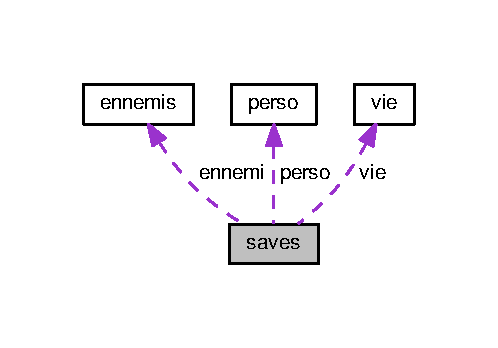
\includegraphics[width=239pt]{structsaves__coll__graph}
\end{center}
\end{figure}
\subsection*{Data Fields}
\begin{DoxyCompactItemize}
\item 
\hyperlink{structperso}{perso} \hyperlink{structsaves_a4ba3cba27704215b96311513ee206401}{perso}
\item 
S\+D\+L\+\_\+\+Rect \hyperlink{structsaves_a4797f7d3b3a1bf30019ec24e4f20b3f1}{camera}
\item 
\hyperlink{structennemis}{ennemis} \hyperlink{structsaves_a94068fb387d61dec9a3f03296d5f2c38}{ennemi}
\item 
\hyperlink{structvie}{vie} \hyperlink{structsaves_ad07a79adf13feb4ffe0f035724ddb04b}{vie}
\item 
int \hyperlink{structsaves_a98a8ba9bd8a8af8f62df3e5f55cbf1a7}{page1}
\item 
int \hyperlink{structsaves_a2d0262e62030f554e86b212e286ce320}{page2}
\item 
int \hyperlink{structsaves_a57efa80fe293ed60438a596d1f42c3b0}{saut}
\item 
int \hyperlink{structsaves_acc2a5ec4f38e63e817228ce80d330cb3}{level}
\end{DoxyCompactItemize}


\subsection{Field Documentation}
\mbox{\Hypertarget{structsaves_a4797f7d3b3a1bf30019ec24e4f20b3f1}\label{structsaves_a4797f7d3b3a1bf30019ec24e4f20b3f1}} 
\index{saves@{saves}!camera@{camera}}
\index{camera@{camera}!saves@{saves}}
\subsubsection{\texorpdfstring{camera}{camera}}
{\footnotesize\ttfamily S\+D\+L\+\_\+\+Rect saves\+::camera}

\mbox{\Hypertarget{structsaves_a94068fb387d61dec9a3f03296d5f2c38}\label{structsaves_a94068fb387d61dec9a3f03296d5f2c38}} 
\index{saves@{saves}!ennemi@{ennemi}}
\index{ennemi@{ennemi}!saves@{saves}}
\subsubsection{\texorpdfstring{ennemi}{ennemi}}
{\footnotesize\ttfamily \hyperlink{structennemis}{ennemis} saves\+::ennemi}

\mbox{\Hypertarget{structsaves_acc2a5ec4f38e63e817228ce80d330cb3}\label{structsaves_acc2a5ec4f38e63e817228ce80d330cb3}} 
\index{saves@{saves}!level@{level}}
\index{level@{level}!saves@{saves}}
\subsubsection{\texorpdfstring{level}{level}}
{\footnotesize\ttfamily int saves\+::level}

\mbox{\Hypertarget{structsaves_a98a8ba9bd8a8af8f62df3e5f55cbf1a7}\label{structsaves_a98a8ba9bd8a8af8f62df3e5f55cbf1a7}} 
\index{saves@{saves}!page1@{page1}}
\index{page1@{page1}!saves@{saves}}
\subsubsection{\texorpdfstring{page1}{page1}}
{\footnotesize\ttfamily int saves\+::page1}

\mbox{\Hypertarget{structsaves_a2d0262e62030f554e86b212e286ce320}\label{structsaves_a2d0262e62030f554e86b212e286ce320}} 
\index{saves@{saves}!page2@{page2}}
\index{page2@{page2}!saves@{saves}}
\subsubsection{\texorpdfstring{page2}{page2}}
{\footnotesize\ttfamily int saves\+::page2}

\mbox{\Hypertarget{structsaves_a4ba3cba27704215b96311513ee206401}\label{structsaves_a4ba3cba27704215b96311513ee206401}} 
\index{saves@{saves}!perso@{perso}}
\index{perso@{perso}!saves@{saves}}
\subsubsection{\texorpdfstring{perso}{perso}}
{\footnotesize\ttfamily \hyperlink{structperso}{perso} saves\+::perso}

\mbox{\Hypertarget{structsaves_a57efa80fe293ed60438a596d1f42c3b0}\label{structsaves_a57efa80fe293ed60438a596d1f42c3b0}} 
\index{saves@{saves}!saut@{saut}}
\index{saut@{saut}!saves@{saves}}
\subsubsection{\texorpdfstring{saut}{saut}}
{\footnotesize\ttfamily int saves\+::saut}

\mbox{\Hypertarget{structsaves_ad07a79adf13feb4ffe0f035724ddb04b}\label{structsaves_ad07a79adf13feb4ffe0f035724ddb04b}} 
\index{saves@{saves}!vie@{vie}}
\index{vie@{vie}!saves@{saves}}
\subsubsection{\texorpdfstring{vie}{vie}}
{\footnotesize\ttfamily \hyperlink{structvie}{vie} saves\+::vie}



The documentation for this struct was generated from the following file\+:\begin{DoxyCompactItemize}
\item 
\hyperlink{level1_8h}{level1.\+h}\end{DoxyCompactItemize}

\hypertarget{structvie}{}\section{vie Struct Reference}
\label{structvie}\index{vie@{vie}}


{\ttfamily \#include $<$perso.\+h$>$}

\subsection*{Data Fields}
\begin{DoxyCompactItemize}
\item 
int \hyperlink{structvie_a02356445cb49a7290950ab15cebccdd9}{nb}
\item 
S\+D\+L\+\_\+\+Rect \hyperlink{structvie_a916050892cf1e7b8039952dcafa44825}{position}
\item 
S\+D\+L\+\_\+\+Rect \hyperlink{structvie_a564dc9c3b28da24d81318d703ebc4e59}{position2}
\item 
S\+D\+L\+\_\+\+Surface $\ast$ \hyperlink{structvie_a7616ae8ecc97b7fb2d92be6a858014ad}{fond1}
\item 
S\+D\+L\+\_\+\+Surface $\ast$ \hyperlink{structvie_a6ecad7f4161cb602faa27d2de9e3ee50}{fond2}
\item 
S\+D\+L\+\_\+\+Surface $\ast$ \hyperlink{structvie_a9763ef794bb12262f5826b911d20e42b}{fond3}
\item 
S\+D\+L\+\_\+\+Surface $\ast$ \hyperlink{structvie_a0b08072b8c7ec9e1adfd6e26b4fcb39f}{fond4}
\item 
S\+D\+L\+\_\+\+Surface $\ast$ \hyperlink{structvie_adabeccdf7e33dd53ac6d85a24fc3931d}{fond5}
\end{DoxyCompactItemize}


\subsection{Field Documentation}
\index{vie@{vie}!fond1@{fond1}}
\index{fond1@{fond1}!vie@{vie}}
\subsubsection[{\texorpdfstring{fond1}{fond1}}]{\setlength{\rightskip}{0pt plus 5cm}S\+D\+L\+\_\+\+Surface$\ast$ vie\+::fond1}\hypertarget{structvie_a7616ae8ecc97b7fb2d92be6a858014ad}{}\label{structvie_a7616ae8ecc97b7fb2d92be6a858014ad}
\index{vie@{vie}!fond2@{fond2}}
\index{fond2@{fond2}!vie@{vie}}
\subsubsection[{\texorpdfstring{fond2}{fond2}}]{\setlength{\rightskip}{0pt plus 5cm}S\+D\+L\+\_\+\+Surface$\ast$ vie\+::fond2}\hypertarget{structvie_a6ecad7f4161cb602faa27d2de9e3ee50}{}\label{structvie_a6ecad7f4161cb602faa27d2de9e3ee50}
\index{vie@{vie}!fond3@{fond3}}
\index{fond3@{fond3}!vie@{vie}}
\subsubsection[{\texorpdfstring{fond3}{fond3}}]{\setlength{\rightskip}{0pt plus 5cm}S\+D\+L\+\_\+\+Surface$\ast$ vie\+::fond3}\hypertarget{structvie_a9763ef794bb12262f5826b911d20e42b}{}\label{structvie_a9763ef794bb12262f5826b911d20e42b}
\index{vie@{vie}!fond4@{fond4}}
\index{fond4@{fond4}!vie@{vie}}
\subsubsection[{\texorpdfstring{fond4}{fond4}}]{\setlength{\rightskip}{0pt plus 5cm}S\+D\+L\+\_\+\+Surface$\ast$ vie\+::fond4}\hypertarget{structvie_a0b08072b8c7ec9e1adfd6e26b4fcb39f}{}\label{structvie_a0b08072b8c7ec9e1adfd6e26b4fcb39f}
\index{vie@{vie}!fond5@{fond5}}
\index{fond5@{fond5}!vie@{vie}}
\subsubsection[{\texorpdfstring{fond5}{fond5}}]{\setlength{\rightskip}{0pt plus 5cm}S\+D\+L\+\_\+\+Surface$\ast$ vie\+::fond5}\hypertarget{structvie_adabeccdf7e33dd53ac6d85a24fc3931d}{}\label{structvie_adabeccdf7e33dd53ac6d85a24fc3931d}
\index{vie@{vie}!nb@{nb}}
\index{nb@{nb}!vie@{vie}}
\subsubsection[{\texorpdfstring{nb}{nb}}]{\setlength{\rightskip}{0pt plus 5cm}int vie\+::nb}\hypertarget{structvie_a02356445cb49a7290950ab15cebccdd9}{}\label{structvie_a02356445cb49a7290950ab15cebccdd9}
\index{vie@{vie}!position@{position}}
\index{position@{position}!vie@{vie}}
\subsubsection[{\texorpdfstring{position}{position}}]{\setlength{\rightskip}{0pt plus 5cm}S\+D\+L\+\_\+\+Rect vie\+::position}\hypertarget{structvie_a916050892cf1e7b8039952dcafa44825}{}\label{structvie_a916050892cf1e7b8039952dcafa44825}
\index{vie@{vie}!position2@{position2}}
\index{position2@{position2}!vie@{vie}}
\subsubsection[{\texorpdfstring{position2}{position2}}]{\setlength{\rightskip}{0pt plus 5cm}S\+D\+L\+\_\+\+Rect vie\+::position2}\hypertarget{structvie_a564dc9c3b28da24d81318d703ebc4e59}{}\label{structvie_a564dc9c3b28da24d81318d703ebc4e59}


The documentation for this struct was generated from the following file\+:\begin{DoxyCompactItemize}
\item 
\hyperlink{perso_8h}{perso.\+h}\end{DoxyCompactItemize}

\chapter{File Documentation}
\hypertarget{collision_8c}{}\section{collision.\+c File Reference}
\label{collision_8c}\index{collision.\+c@{collision.\+c}}
{\ttfamily \#include \char`\"{}fonction.\+h\char`\"{}}\newline
Include dependency graph for collision.\+c\+:\nopagebreak
\begin{figure}[H]
\begin{center}
\leavevmode
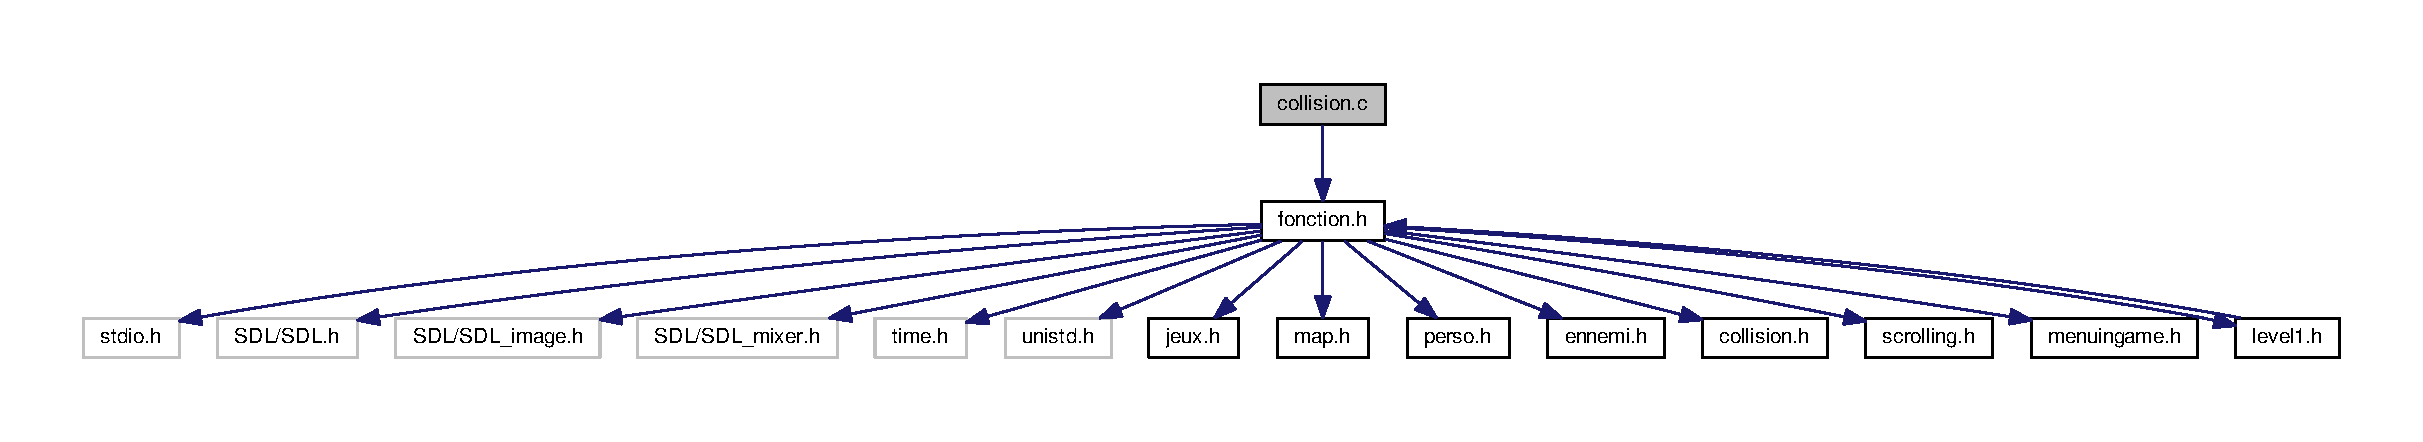
\includegraphics[width=350pt]{collision_8c__incl}
\end{center}
\end{figure}
\subsection*{Functions}
\begin{DoxyCompactItemize}
\item 
Uint32 \hyperlink{collision_8c_a62e59210ffa856d8cc4443972ab6b49f}{getpixel} (S\+D\+L\+\_\+\+Surface $\ast$surface, int x, int y)
\item 
S\+D\+L\+\_\+\+Rect \hyperlink{collision_8c_a622a012cafa9f1d28d7acbd6f54d035b}{collision} (S\+D\+L\+\_\+\+Rect camera, \hyperlink{structperso}{perso} \hyperlink{structperso}{perso})
\item 
int \hyperlink{collision_8c_a03dc9846b7bb33f17ba5e95642a7eae8}{collisionescalier} (\hyperlink{structperso}{perso} \hyperlink{structperso}{perso}, \hyperlink{structescalier}{escalier} \hyperlink{structescalier}{escalier}, S\+D\+L\+\_\+\+Rect camera)
\item 
void \hyperlink{collision_8c_a5d0442d691e0654d51f1019b9e1a10b6}{collisionennemi} (\hyperlink{structperso}{perso} $\ast$\hyperlink{structperso}{perso}, \hyperlink{structennemis}{ennemis} $\ast$ennemi, S\+D\+L\+\_\+\+Rect $\ast$camera, \hyperlink{structvie}{vie} $\ast$\hyperlink{structvie}{vie})
\end{DoxyCompactItemize}


\subsection{Function Documentation}
\mbox{\Hypertarget{collision_8c_a622a012cafa9f1d28d7acbd6f54d035b}\label{collision_8c_a622a012cafa9f1d28d7acbd6f54d035b}} 
\index{collision.\+c@{collision.\+c}!collision@{collision}}
\index{collision@{collision}!collision.\+c@{collision.\+c}}
\subsubsection{\texorpdfstring{collision()}{collision()}}
{\footnotesize\ttfamily S\+D\+L\+\_\+\+Rect collision (\begin{DoxyParamCaption}\item[{S\+D\+L\+\_\+\+Rect}]{camera,  }\item[{\hyperlink{structperso}{perso}}]{perso }\end{DoxyParamCaption})}

Here is the caller graph for this function\+:\nopagebreak
\begin{figure}[H]
\begin{center}
\leavevmode
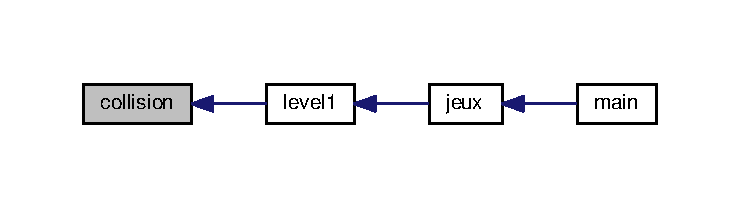
\includegraphics[width=350pt]{collision_8c_a622a012cafa9f1d28d7acbd6f54d035b_icgraph}
\end{center}
\end{figure}
\mbox{\Hypertarget{collision_8c_a5d0442d691e0654d51f1019b9e1a10b6}\label{collision_8c_a5d0442d691e0654d51f1019b9e1a10b6}} 
\index{collision.\+c@{collision.\+c}!collisionennemi@{collisionennemi}}
\index{collisionennemi@{collisionennemi}!collision.\+c@{collision.\+c}}
\subsubsection{\texorpdfstring{collisionennemi()}{collisionennemi()}}
{\footnotesize\ttfamily void collisionennemi (\begin{DoxyParamCaption}\item[{\hyperlink{structperso}{perso} $\ast$}]{perso,  }\item[{\hyperlink{structennemis}{ennemis} $\ast$}]{ennemi,  }\item[{S\+D\+L\+\_\+\+Rect $\ast$}]{camera,  }\item[{\hyperlink{structvie}{vie} $\ast$}]{vie }\end{DoxyParamCaption})}

Here is the caller graph for this function\+:\nopagebreak
\begin{figure}[H]
\begin{center}
\leavevmode
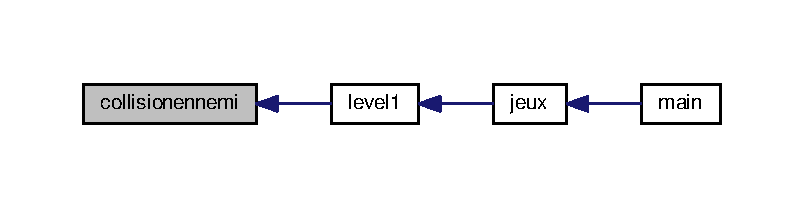
\includegraphics[width=350pt]{collision_8c_a5d0442d691e0654d51f1019b9e1a10b6_icgraph}
\end{center}
\end{figure}
\mbox{\Hypertarget{collision_8c_a03dc9846b7bb33f17ba5e95642a7eae8}\label{collision_8c_a03dc9846b7bb33f17ba5e95642a7eae8}} 
\index{collision.\+c@{collision.\+c}!collisionescalier@{collisionescalier}}
\index{collisionescalier@{collisionescalier}!collision.\+c@{collision.\+c}}
\subsubsection{\texorpdfstring{collisionescalier()}{collisionescalier()}}
{\footnotesize\ttfamily int collisionescalier (\begin{DoxyParamCaption}\item[{\hyperlink{structperso}{perso}}]{perso,  }\item[{\hyperlink{structescalier}{escalier}}]{escalier,  }\item[{S\+D\+L\+\_\+\+Rect}]{camera }\end{DoxyParamCaption})}

Here is the call graph for this function\+:\nopagebreak
\begin{figure}[H]
\begin{center}
\leavevmode
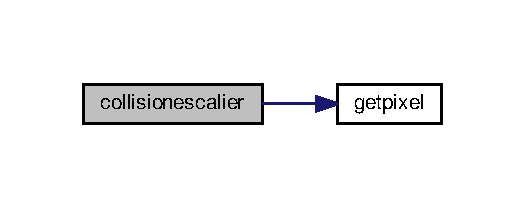
\includegraphics[width=252pt]{collision_8c_a03dc9846b7bb33f17ba5e95642a7eae8_cgraph}
\end{center}
\end{figure}
Here is the caller graph for this function\+:\nopagebreak
\begin{figure}[H]
\begin{center}
\leavevmode
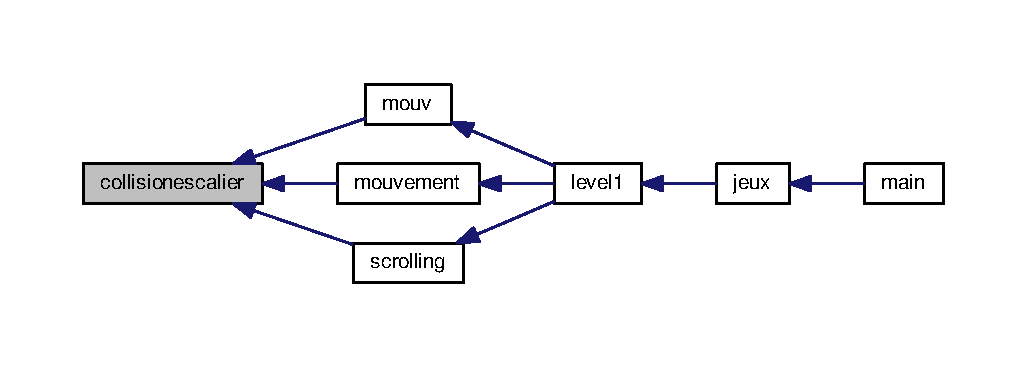
\includegraphics[width=350pt]{collision_8c_a03dc9846b7bb33f17ba5e95642a7eae8_icgraph}
\end{center}
\end{figure}
\mbox{\Hypertarget{collision_8c_a62e59210ffa856d8cc4443972ab6b49f}\label{collision_8c_a62e59210ffa856d8cc4443972ab6b49f}} 
\index{collision.\+c@{collision.\+c}!getpixel@{getpixel}}
\index{getpixel@{getpixel}!collision.\+c@{collision.\+c}}
\subsubsection{\texorpdfstring{getpixel()}{getpixel()}}
{\footnotesize\ttfamily Uint32 getpixel (\begin{DoxyParamCaption}\item[{S\+D\+L\+\_\+\+Surface $\ast$}]{surface,  }\item[{int}]{x,  }\item[{int}]{y }\end{DoxyParamCaption})}

Here is the caller graph for this function\+:\nopagebreak
\begin{figure}[H]
\begin{center}
\leavevmode
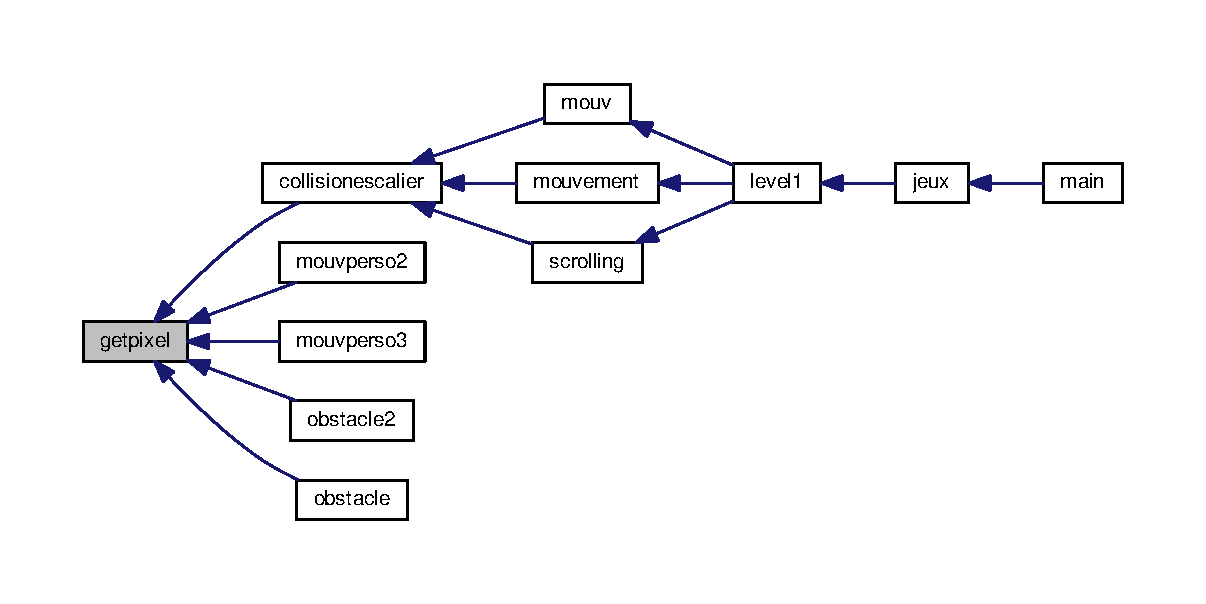
\includegraphics[width=350pt]{collision_8c_a62e59210ffa856d8cc4443972ab6b49f_icgraph}
\end{center}
\end{figure}

\hypertarget{collision_8h}{}\section{collision.\+h File Reference}
\label{collision_8h}\index{collision.\+h@{collision.\+h}}
This graph shows which files directly or indirectly include this file\+:
\nopagebreak
\begin{figure}[H]
\begin{center}
\leavevmode
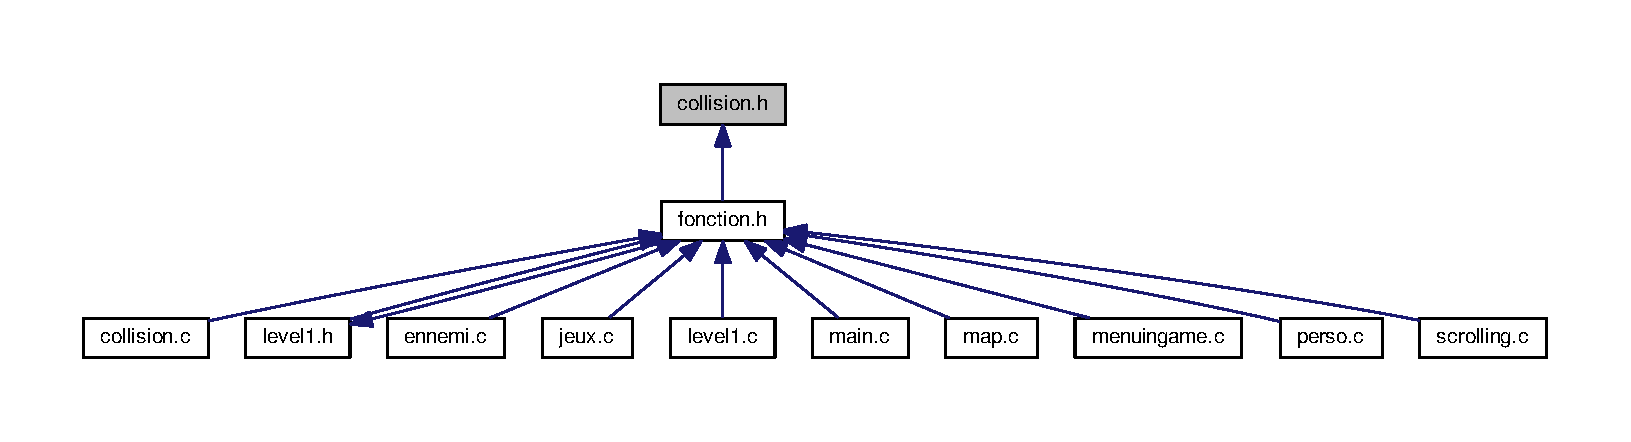
\includegraphics[width=350pt]{collision_8h__dep__incl}
\end{center}
\end{figure}
\subsection*{Functions}
\begin{DoxyCompactItemize}
\item 
Uint32 \hyperlink{collision_8h_a62e59210ffa856d8cc4443972ab6b49f}{getpixel} (S\+D\+L\+\_\+\+Surface $\ast$surface, int x, int y)
\item 
S\+D\+L\+\_\+\+Rect \hyperlink{collision_8h_a622a012cafa9f1d28d7acbd6f54d035b}{collision} (S\+D\+L\+\_\+\+Rect camera, \hyperlink{structperso}{perso} \hyperlink{structperso}{perso})
\item 
int \hyperlink{collision_8h_a03dc9846b7bb33f17ba5e95642a7eae8}{collisionescalier} (\hyperlink{structperso}{perso} \hyperlink{structperso}{perso}, \hyperlink{structescalier}{escalier} \hyperlink{structescalier}{escalier}, S\+D\+L\+\_\+\+Rect camera)
\item 
void \hyperlink{collision_8h_a5d0442d691e0654d51f1019b9e1a10b6}{collisionennemi} (\hyperlink{structperso}{perso} $\ast$\hyperlink{structperso}{perso}, \hyperlink{structennemis}{ennemis} $\ast$ennemi, S\+D\+L\+\_\+\+Rect $\ast$camera, \hyperlink{structvie}{vie} $\ast$\hyperlink{structvie}{vie})
\end{DoxyCompactItemize}


\subsection{Function Documentation}
\index{collision.\+h@{collision.\+h}!collision@{collision}}
\index{collision@{collision}!collision.\+h@{collision.\+h}}
\subsubsection[{\texorpdfstring{collision(\+S\+D\+L\+\_\+\+Rect camera, perso perso)}{collision(SDL_Rect camera, perso perso)}}]{\setlength{\rightskip}{0pt plus 5cm}S\+D\+L\+\_\+\+Rect collision (
\begin{DoxyParamCaption}
\item[{S\+D\+L\+\_\+\+Rect}]{camera, }
\item[{{\bf perso}}]{perso}
\end{DoxyParamCaption}
)}\hypertarget{collision_8h_a622a012cafa9f1d28d7acbd6f54d035b}{}\label{collision_8h_a622a012cafa9f1d28d7acbd6f54d035b}


Here is the caller graph for this function\+:
\nopagebreak
\begin{figure}[H]
\begin{center}
\leavevmode
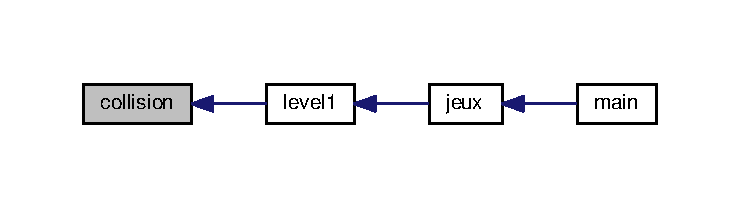
\includegraphics[width=350pt]{collision_8h_a622a012cafa9f1d28d7acbd6f54d035b_icgraph}
\end{center}
\end{figure}


\index{collision.\+h@{collision.\+h}!collisionennemi@{collisionennemi}}
\index{collisionennemi@{collisionennemi}!collision.\+h@{collision.\+h}}
\subsubsection[{\texorpdfstring{collisionennemi(perso $\ast$perso, ennemis $\ast$ennemi, S\+D\+L\+\_\+\+Rect $\ast$camera, vie $\ast$vie)}{collisionennemi(perso *perso, ennemis *ennemi, SDL_Rect *camera, vie *vie)}}]{\setlength{\rightskip}{0pt plus 5cm}void collisionennemi (
\begin{DoxyParamCaption}
\item[{{\bf perso} $\ast$}]{perso, }
\item[{{\bf ennemis} $\ast$}]{ennemi, }
\item[{S\+D\+L\+\_\+\+Rect $\ast$}]{camera, }
\item[{{\bf vie} $\ast$}]{vie}
\end{DoxyParamCaption}
)}\hypertarget{collision_8h_a5d0442d691e0654d51f1019b9e1a10b6}{}\label{collision_8h_a5d0442d691e0654d51f1019b9e1a10b6}


Here is the caller graph for this function\+:
\nopagebreak
\begin{figure}[H]
\begin{center}
\leavevmode
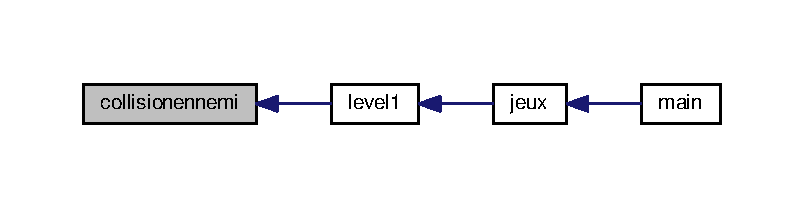
\includegraphics[width=350pt]{collision_8h_a5d0442d691e0654d51f1019b9e1a10b6_icgraph}
\end{center}
\end{figure}


\index{collision.\+h@{collision.\+h}!collisionescalier@{collisionescalier}}
\index{collisionescalier@{collisionescalier}!collision.\+h@{collision.\+h}}
\subsubsection[{\texorpdfstring{collisionescalier(perso perso, escalier escalier, S\+D\+L\+\_\+\+Rect camera)}{collisionescalier(perso perso, escalier escalier, SDL_Rect camera)}}]{\setlength{\rightskip}{0pt plus 5cm}int collisionescalier (
\begin{DoxyParamCaption}
\item[{{\bf perso}}]{perso, }
\item[{{\bf escalier}}]{escalier, }
\item[{S\+D\+L\+\_\+\+Rect}]{camera}
\end{DoxyParamCaption}
)}\hypertarget{collision_8h_a03dc9846b7bb33f17ba5e95642a7eae8}{}\label{collision_8h_a03dc9846b7bb33f17ba5e95642a7eae8}


Here is the call graph for this function\+:
\nopagebreak
\begin{figure}[H]
\begin{center}
\leavevmode
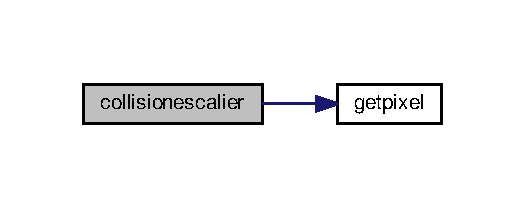
\includegraphics[width=252pt]{collision_8h_a03dc9846b7bb33f17ba5e95642a7eae8_cgraph}
\end{center}
\end{figure}




Here is the caller graph for this function\+:
\nopagebreak
\begin{figure}[H]
\begin{center}
\leavevmode
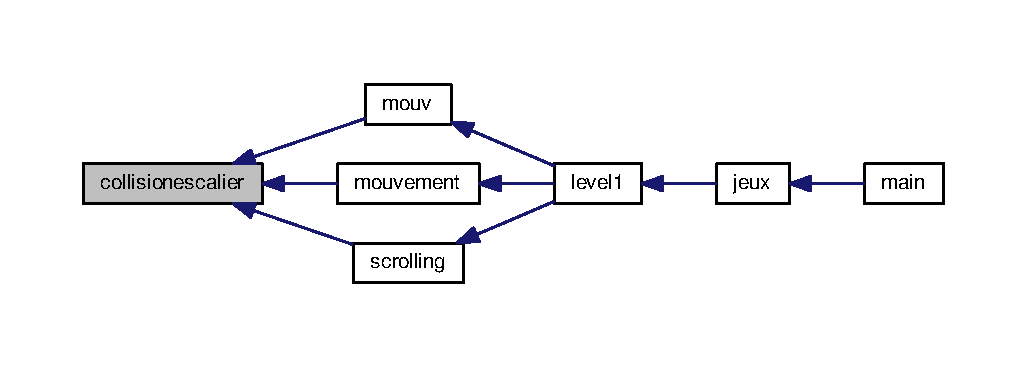
\includegraphics[width=350pt]{collision_8h_a03dc9846b7bb33f17ba5e95642a7eae8_icgraph}
\end{center}
\end{figure}


\index{collision.\+h@{collision.\+h}!getpixel@{getpixel}}
\index{getpixel@{getpixel}!collision.\+h@{collision.\+h}}
\subsubsection[{\texorpdfstring{getpixel(\+S\+D\+L\+\_\+\+Surface $\ast$surface, int x, int y)}{getpixel(SDL_Surface *surface, int x, int y)}}]{\setlength{\rightskip}{0pt plus 5cm}Uint32 getpixel (
\begin{DoxyParamCaption}
\item[{S\+D\+L\+\_\+\+Surface $\ast$}]{surface, }
\item[{int}]{x, }
\item[{int}]{y}
\end{DoxyParamCaption}
)}\hypertarget{collision_8h_a62e59210ffa856d8cc4443972ab6b49f}{}\label{collision_8h_a62e59210ffa856d8cc4443972ab6b49f}


Here is the caller graph for this function\+:
\nopagebreak
\begin{figure}[H]
\begin{center}
\leavevmode
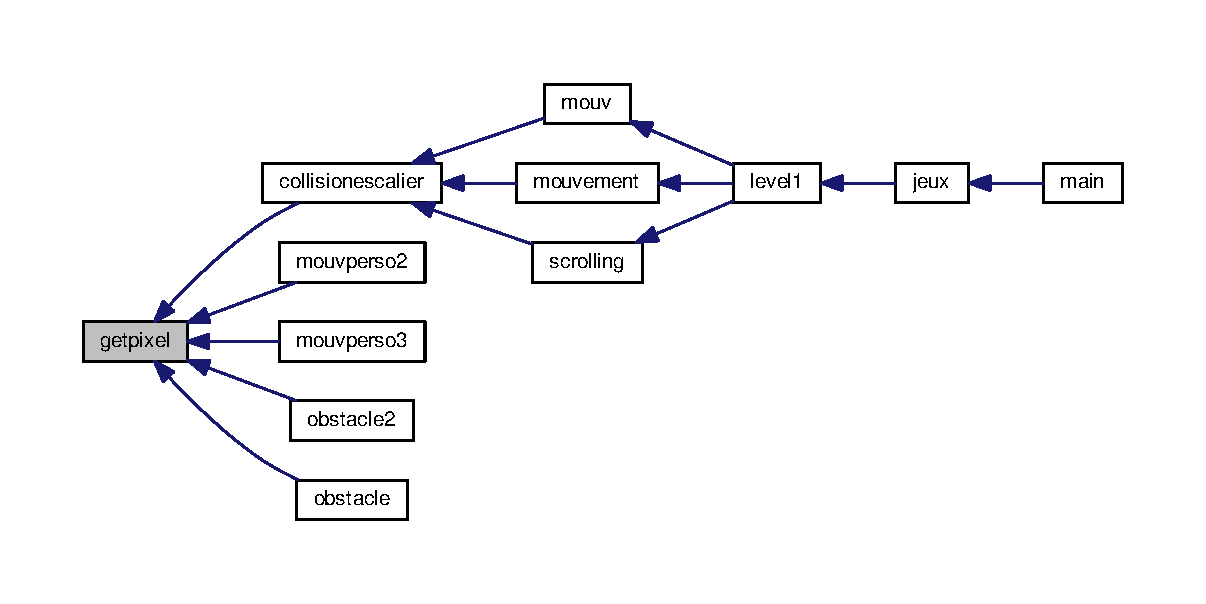
\includegraphics[width=350pt]{collision_8h_a62e59210ffa856d8cc4443972ab6b49f_icgraph}
\end{center}
\end{figure}



\hypertarget{enigme_8c}{}\section{enigme.\+c File Reference}
\label{enigme_8c}\index{enigme.\+c@{enigme.\+c}}
{\ttfamily \#include $<$stdio.\+h$>$}\newline
{\ttfamily \#include $<$stdlib.\+h$>$}\newline
{\ttfamily \#include $<$string.\+h$>$}\newline
{\ttfamily \#include $<$S\+D\+L/\+S\+D\+L.\+h$>$}\newline
{\ttfamily \#include $<$S\+D\+L/\+S\+D\+L\+\_\+mixer.\+h$>$}\newline
{\ttfamily \#include $<$S\+D\+L/\+S\+D\+L\+\_\+image.\+h$>$}\newline
{\ttfamily \#include \char`\"{}enigme.\+h\char`\"{}}\newline
Include dependency graph for enigme.\+c\+:\nopagebreak
\begin{figure}[H]
\begin{center}
\leavevmode
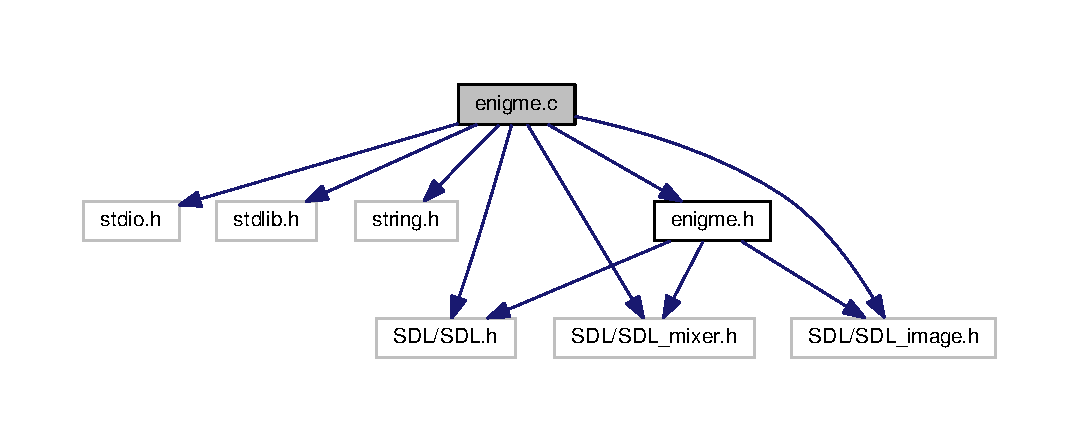
\includegraphics[width=350pt]{enigme_8c__incl}
\end{center}
\end{figure}
\subsection*{Functions}
\begin{DoxyCompactItemize}
\item 
void \hyperlink{enigme_8c_ad454a117b28e1ea763edf855960bf66a}{init\+\_\+enigme} (\hyperlink{structenigme}{enigme} $\ast$enig)
\item 
void \hyperlink{enigme_8c_a3f9c87b77c1f75c892dee0fe1de7c5d7}{generate\+\_\+afficher} (S\+D\+L\+\_\+\+Surface $\ast$ecran, char image \mbox{[}$\,$\mbox{]}, \hyperlink{structenigme}{enigme} $\ast$enig, int $\ast$alea)
\item 
int \hyperlink{enigme_8c_a35379216444e495869c21407672218a2}{solution\+\_\+e} (char image \mbox{[}$\,$\mbox{]})
\item 
int \hyperlink{enigme_8c_ae855a03b9d7f7619bac3843306965df9}{resolution} (int $\ast$running, int $\ast$run)
\item 
void \hyperlink{enigme_8c_ac0874aeffd6ff2e1b39ae34e1d7d8618}{afficher\+\_\+resultat} (S\+D\+L\+\_\+\+Surface $\ast$ecran, int sol, int r, \hyperlink{structenigme}{enigme} $\ast$en)
\end{DoxyCompactItemize}


\subsection{Function Documentation}
\mbox{\Hypertarget{enigme_8c_ac0874aeffd6ff2e1b39ae34e1d7d8618}\label{enigme_8c_ac0874aeffd6ff2e1b39ae34e1d7d8618}} 
\index{enigme.\+c@{enigme.\+c}!afficher\+\_\+resultat@{afficher\+\_\+resultat}}
\index{afficher\+\_\+resultat@{afficher\+\_\+resultat}!enigme.\+c@{enigme.\+c}}
\subsubsection{\texorpdfstring{afficher\+\_\+resultat()}{afficher\_resultat()}}
{\footnotesize\ttfamily void afficher\+\_\+resultat (\begin{DoxyParamCaption}\item[{S\+D\+L\+\_\+\+Surface $\ast$}]{ecran,  }\item[{int}]{sol,  }\item[{int}]{r,  }\item[{\hyperlink{structenigme}{enigme} $\ast$}]{en }\end{DoxyParamCaption})}

\mbox{\Hypertarget{enigme_8c_a3f9c87b77c1f75c892dee0fe1de7c5d7}\label{enigme_8c_a3f9c87b77c1f75c892dee0fe1de7c5d7}} 
\index{enigme.\+c@{enigme.\+c}!generate\+\_\+afficher@{generate\+\_\+afficher}}
\index{generate\+\_\+afficher@{generate\+\_\+afficher}!enigme.\+c@{enigme.\+c}}
\subsubsection{\texorpdfstring{generate\+\_\+afficher()}{generate\_afficher()}}
{\footnotesize\ttfamily void generate\+\_\+afficher (\begin{DoxyParamCaption}\item[{S\+D\+L\+\_\+\+Surface $\ast$}]{ecran,  }\item[{char}]{image\mbox{[}$\,$\mbox{]},  }\item[{\hyperlink{structenigme}{enigme} $\ast$}]{enig,  }\item[{int $\ast$}]{alea }\end{DoxyParamCaption})}

\mbox{\Hypertarget{enigme_8c_ad454a117b28e1ea763edf855960bf66a}\label{enigme_8c_ad454a117b28e1ea763edf855960bf66a}} 
\index{enigme.\+c@{enigme.\+c}!init\+\_\+enigme@{init\+\_\+enigme}}
\index{init\+\_\+enigme@{init\+\_\+enigme}!enigme.\+c@{enigme.\+c}}
\subsubsection{\texorpdfstring{init\+\_\+enigme()}{init\_enigme()}}
{\footnotesize\ttfamily void init\+\_\+enigme (\begin{DoxyParamCaption}\item[{\hyperlink{structenigme}{enigme} $\ast$}]{enig }\end{DoxyParamCaption})}

\mbox{\Hypertarget{enigme_8c_ae855a03b9d7f7619bac3843306965df9}\label{enigme_8c_ae855a03b9d7f7619bac3843306965df9}} 
\index{enigme.\+c@{enigme.\+c}!resolution@{resolution}}
\index{resolution@{resolution}!enigme.\+c@{enigme.\+c}}
\subsubsection{\texorpdfstring{resolution()}{resolution()}}
{\footnotesize\ttfamily int resolution (\begin{DoxyParamCaption}\item[{int $\ast$}]{running,  }\item[{int $\ast$}]{run }\end{DoxyParamCaption})}

\mbox{\Hypertarget{enigme_8c_a35379216444e495869c21407672218a2}\label{enigme_8c_a35379216444e495869c21407672218a2}} 
\index{enigme.\+c@{enigme.\+c}!solution\+\_\+e@{solution\+\_\+e}}
\index{solution\+\_\+e@{solution\+\_\+e}!enigme.\+c@{enigme.\+c}}
\subsubsection{\texorpdfstring{solution\+\_\+e()}{solution\_e()}}
{\footnotesize\ttfamily int solution\+\_\+e (\begin{DoxyParamCaption}\item[{char}]{image\mbox{[}$\,$\mbox{]} }\end{DoxyParamCaption})}


\hypertarget{enigme_8h}{}\section{enigme.\+h File Reference}
\label{enigme_8h}\index{enigme.\+h@{enigme.\+h}}
{\ttfamily \#include $<$S\+D\+L/\+S\+D\+L.\+h$>$}\\*
{\ttfamily \#include $<$S\+D\+L/\+S\+D\+L\+\_\+mixer.\+h$>$}\\*
{\ttfamily \#include $<$S\+D\+L/\+S\+D\+L\+\_\+image.\+h$>$}\\*
Include dependency graph for enigme.\+h\+:
\nopagebreak
\begin{figure}[H]
\begin{center}
\leavevmode
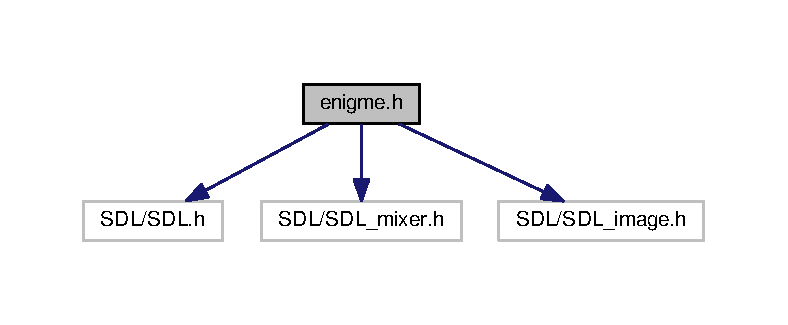
\includegraphics[width=350pt]{enigme_8h__incl}
\end{center}
\end{figure}
This graph shows which files directly or indirectly include this file\+:
\nopagebreak
\begin{figure}[H]
\begin{center}
\leavevmode
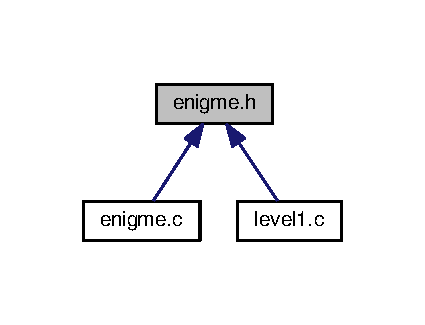
\includegraphics[width=204pt]{enigme_8h__dep__incl}
\end{center}
\end{figure}
\subsection*{Data Structures}
\begin{DoxyCompactItemize}
\item 
struct \hyperlink{structenigme}{enigme}
\end{DoxyCompactItemize}
\subsection*{Functions}
\begin{DoxyCompactItemize}
\item 
void \hyperlink{enigme_8h_ad454a117b28e1ea763edf855960bf66a}{init\+\_\+enigme} (\hyperlink{structenigme}{enigme} $\ast$enig)
\item 
void \hyperlink{enigme_8h_a3a50a6a4011cda91784c0bcfa053c103}{generate\+\_\+afficher} (S\+D\+L\+\_\+\+Surface $\ast$ecran, char image\mbox{[}$\,$\mbox{]}, \hyperlink{structenigme}{enigme} $\ast$enig, int $\ast$alea)
\item 
int \hyperlink{enigme_8h_a9747794ee1668739d447baf139b1fcec}{solution\+\_\+e} (char image\mbox{[}$\,$\mbox{]})
\item 
int \hyperlink{enigme_8h_ae855a03b9d7f7619bac3843306965df9}{resolution} (int $\ast$running, int $\ast$run)
\item 
void \hyperlink{enigme_8h_ac0874aeffd6ff2e1b39ae34e1d7d8618}{afficher\+\_\+resultat} (S\+D\+L\+\_\+\+Surface $\ast$ecran, int sol, int r, \hyperlink{structenigme}{enigme} $\ast$en)
\end{DoxyCompactItemize}


\subsection{Function Documentation}
\index{enigme.\+h@{enigme.\+h}!afficher\+\_\+resultat@{afficher\+\_\+resultat}}
\index{afficher\+\_\+resultat@{afficher\+\_\+resultat}!enigme.\+h@{enigme.\+h}}
\subsubsection[{\texorpdfstring{afficher\+\_\+resultat(\+S\+D\+L\+\_\+\+Surface $\ast$ecran, int sol, int r, enigme $\ast$en)}{afficher_resultat(SDL_Surface *ecran, int sol, int r, enigme *en)}}]{\setlength{\rightskip}{0pt plus 5cm}void afficher\+\_\+resultat (
\begin{DoxyParamCaption}
\item[{S\+D\+L\+\_\+\+Surface $\ast$}]{ecran, }
\item[{int}]{sol, }
\item[{int}]{r, }
\item[{{\bf enigme} $\ast$}]{en}
\end{DoxyParamCaption}
)}\hypertarget{enigme_8h_ac0874aeffd6ff2e1b39ae34e1d7d8618}{}\label{enigme_8h_ac0874aeffd6ff2e1b39ae34e1d7d8618}


Here is the caller graph for this function\+:
\nopagebreak
\begin{figure}[H]
\begin{center}
\leavevmode
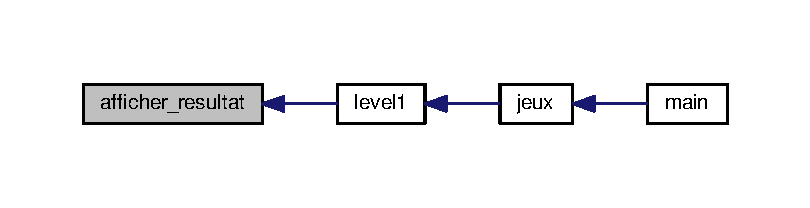
\includegraphics[width=350pt]{enigme_8h_ac0874aeffd6ff2e1b39ae34e1d7d8618_icgraph}
\end{center}
\end{figure}


\index{enigme.\+h@{enigme.\+h}!generate\+\_\+afficher@{generate\+\_\+afficher}}
\index{generate\+\_\+afficher@{generate\+\_\+afficher}!enigme.\+h@{enigme.\+h}}
\subsubsection[{\texorpdfstring{generate\+\_\+afficher(\+S\+D\+L\+\_\+\+Surface $\ast$ecran, char image[], enigme $\ast$enig, int $\ast$alea)}{generate_afficher(SDL_Surface *ecran, char image[], enigme *enig, int *alea)}}]{\setlength{\rightskip}{0pt plus 5cm}void generate\+\_\+afficher (
\begin{DoxyParamCaption}
\item[{S\+D\+L\+\_\+\+Surface $\ast$}]{ecran, }
\item[{char}]{image\mbox{[}$\,$\mbox{]}, }
\item[{{\bf enigme} $\ast$}]{enig, }
\item[{int $\ast$}]{alea}
\end{DoxyParamCaption}
)}\hypertarget{enigme_8h_a3a50a6a4011cda91784c0bcfa053c103}{}\label{enigme_8h_a3a50a6a4011cda91784c0bcfa053c103}


Here is the caller graph for this function\+:
\nopagebreak
\begin{figure}[H]
\begin{center}
\leavevmode
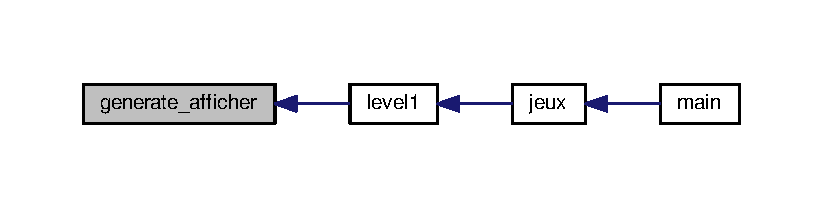
\includegraphics[width=350pt]{enigme_8h_a3a50a6a4011cda91784c0bcfa053c103_icgraph}
\end{center}
\end{figure}


\index{enigme.\+h@{enigme.\+h}!init\+\_\+enigme@{init\+\_\+enigme}}
\index{init\+\_\+enigme@{init\+\_\+enigme}!enigme.\+h@{enigme.\+h}}
\subsubsection[{\texorpdfstring{init\+\_\+enigme(enigme $\ast$enig)}{init_enigme(enigme *enig)}}]{\setlength{\rightskip}{0pt plus 5cm}void init\+\_\+enigme (
\begin{DoxyParamCaption}
\item[{{\bf enigme} $\ast$}]{enig}
\end{DoxyParamCaption}
)}\hypertarget{enigme_8h_ad454a117b28e1ea763edf855960bf66a}{}\label{enigme_8h_ad454a117b28e1ea763edf855960bf66a}


Here is the caller graph for this function\+:
\nopagebreak
\begin{figure}[H]
\begin{center}
\leavevmode
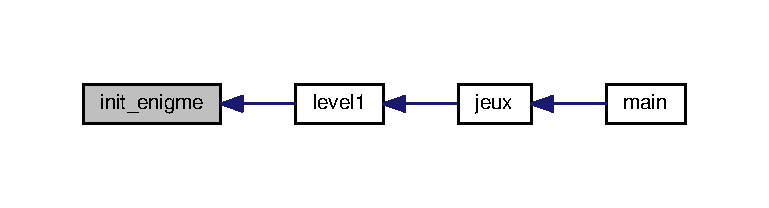
\includegraphics[width=350pt]{enigme_8h_ad454a117b28e1ea763edf855960bf66a_icgraph}
\end{center}
\end{figure}


\index{enigme.\+h@{enigme.\+h}!resolution@{resolution}}
\index{resolution@{resolution}!enigme.\+h@{enigme.\+h}}
\subsubsection[{\texorpdfstring{resolution(int $\ast$running, int $\ast$run)}{resolution(int *running, int *run)}}]{\setlength{\rightskip}{0pt plus 5cm}int resolution (
\begin{DoxyParamCaption}
\item[{int $\ast$}]{running, }
\item[{int $\ast$}]{run}
\end{DoxyParamCaption}
)}\hypertarget{enigme_8h_ae855a03b9d7f7619bac3843306965df9}{}\label{enigme_8h_ae855a03b9d7f7619bac3843306965df9}


Here is the caller graph for this function\+:
\nopagebreak
\begin{figure}[H]
\begin{center}
\leavevmode
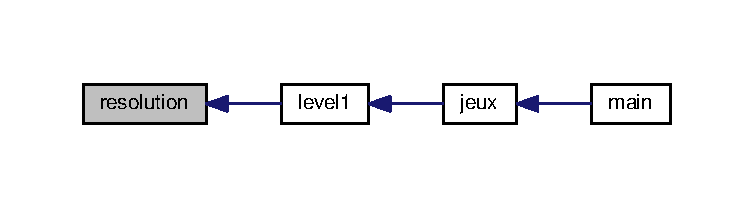
\includegraphics[width=350pt]{enigme_8h_ae855a03b9d7f7619bac3843306965df9_icgraph}
\end{center}
\end{figure}


\index{enigme.\+h@{enigme.\+h}!solution\+\_\+e@{solution\+\_\+e}}
\index{solution\+\_\+e@{solution\+\_\+e}!enigme.\+h@{enigme.\+h}}
\subsubsection[{\texorpdfstring{solution\+\_\+e(char image[])}{solution_e(char image[])}}]{\setlength{\rightskip}{0pt plus 5cm}int solution\+\_\+e (
\begin{DoxyParamCaption}
\item[{char}]{image\mbox{[}$\,$\mbox{]}}
\end{DoxyParamCaption}
)}\hypertarget{enigme_8h_a9747794ee1668739d447baf139b1fcec}{}\label{enigme_8h_a9747794ee1668739d447baf139b1fcec}

\hypertarget{ennemi_8c}{}\section{ennemi.\+c File Reference}
\label{ennemi_8c}\index{ennemi.\+c@{ennemi.\+c}}
{\ttfamily \#include \char`\"{}fonction.\+h\char`\"{}}\newline
Include dependency graph for ennemi.\+c\+:\nopagebreak
\begin{figure}[H]
\begin{center}
\leavevmode
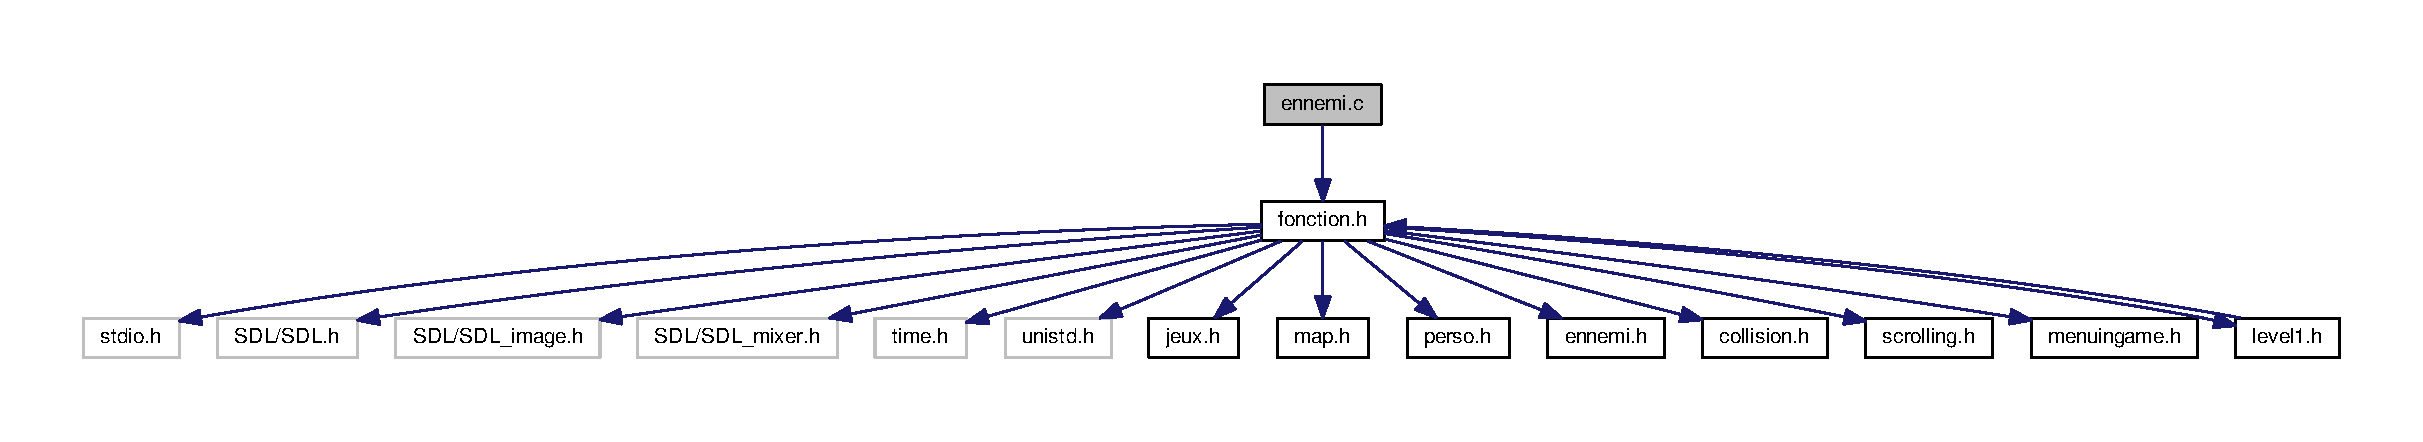
\includegraphics[width=350pt]{ennemi_8c__incl}
\end{center}
\end{figure}
\subsection*{Functions}
\begin{DoxyCompactItemize}
\item 
void \hyperlink{ennemi_8c_a7e97b6df5122a4ba309bff21a456dafa}{initialiserennemi} (\hyperlink{structennemis}{ennemis} $\ast$ennemi)
\item 
void \hyperlink{ennemi_8c_ac2414a6bd133a4ad2668dae5a823cdb3}{freesurfaceennemi} (\hyperlink{structennemis}{ennemis} $\ast$ennemi)
\item 
\hyperlink{structennemis}{ennemis} \hyperlink{ennemi_8c_affe5e211a9cd4ecb89ed255a8f28e9f5}{mouvennemi} (\hyperlink{structennemis}{ennemis} ennemi, \hyperlink{structperso}{perso} \hyperlink{structperso}{perso}, int d, int q, S\+D\+L\+\_\+\+Rect camera, S\+D\+L\+\_\+\+Surface $\ast$ecran, int $\ast$ennmouv, int $\ast$w, int $\ast$y, int mvmspeed)
\item 
int \hyperlink{ennemi_8c_aebc98d93ce6c740a80cfe951a2303af9}{splitennemi} (int y)
\item 
void \hyperlink{ennemi_8c_a3dc49b6654ac3b32977ce5ba4901c498}{afficherennemi} (\hyperlink{structennemis}{ennemis} ennemi, S\+D\+L\+\_\+\+Surface $\ast$ecran, int y)
\end{DoxyCompactItemize}


\subsection{Function Documentation}
\mbox{\Hypertarget{ennemi_8c_a3dc49b6654ac3b32977ce5ba4901c498}\label{ennemi_8c_a3dc49b6654ac3b32977ce5ba4901c498}} 
\index{ennemi.\+c@{ennemi.\+c}!afficherennemi@{afficherennemi}}
\index{afficherennemi@{afficherennemi}!ennemi.\+c@{ennemi.\+c}}
\subsubsection{\texorpdfstring{afficherennemi()}{afficherennemi()}}
{\footnotesize\ttfamily void afficherennemi (\begin{DoxyParamCaption}\item[{\hyperlink{structennemis}{ennemis}}]{ennemi,  }\item[{S\+D\+L\+\_\+\+Surface $\ast$}]{ecran,  }\item[{int}]{y }\end{DoxyParamCaption})}

Here is the caller graph for this function\+:\nopagebreak
\begin{figure}[H]
\begin{center}
\leavevmode
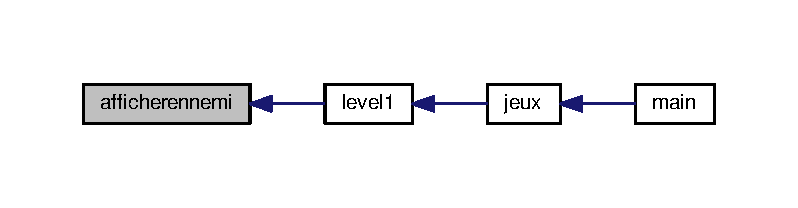
\includegraphics[width=350pt]{ennemi_8c_a3dc49b6654ac3b32977ce5ba4901c498_icgraph}
\end{center}
\end{figure}
\mbox{\Hypertarget{ennemi_8c_ac2414a6bd133a4ad2668dae5a823cdb3}\label{ennemi_8c_ac2414a6bd133a4ad2668dae5a823cdb3}} 
\index{ennemi.\+c@{ennemi.\+c}!freesurfaceennemi@{freesurfaceennemi}}
\index{freesurfaceennemi@{freesurfaceennemi}!ennemi.\+c@{ennemi.\+c}}
\subsubsection{\texorpdfstring{freesurfaceennemi()}{freesurfaceennemi()}}
{\footnotesize\ttfamily void freesurfaceennemi (\begin{DoxyParamCaption}\item[{\hyperlink{structennemis}{ennemis} $\ast$}]{ennemi }\end{DoxyParamCaption})}

Here is the caller graph for this function\+:\nopagebreak
\begin{figure}[H]
\begin{center}
\leavevmode
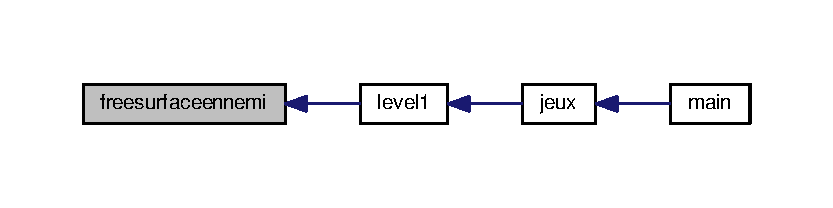
\includegraphics[width=350pt]{ennemi_8c_ac2414a6bd133a4ad2668dae5a823cdb3_icgraph}
\end{center}
\end{figure}
\mbox{\Hypertarget{ennemi_8c_a7e97b6df5122a4ba309bff21a456dafa}\label{ennemi_8c_a7e97b6df5122a4ba309bff21a456dafa}} 
\index{ennemi.\+c@{ennemi.\+c}!initialiserennemi@{initialiserennemi}}
\index{initialiserennemi@{initialiserennemi}!ennemi.\+c@{ennemi.\+c}}
\subsubsection{\texorpdfstring{initialiserennemi()}{initialiserennemi()}}
{\footnotesize\ttfamily void initialiserennemi (\begin{DoxyParamCaption}\item[{\hyperlink{structennemis}{ennemis} $\ast$}]{ennemi }\end{DoxyParamCaption})}

Here is the caller graph for this function\+:\nopagebreak
\begin{figure}[H]
\begin{center}
\leavevmode
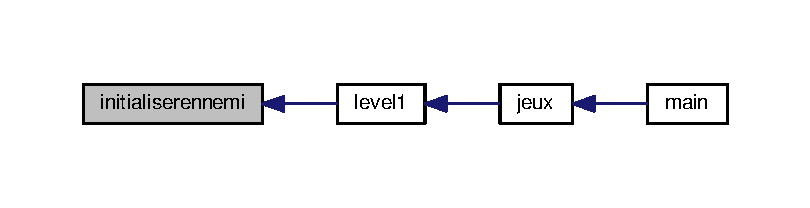
\includegraphics[width=350pt]{ennemi_8c_a7e97b6df5122a4ba309bff21a456dafa_icgraph}
\end{center}
\end{figure}
\mbox{\Hypertarget{ennemi_8c_affe5e211a9cd4ecb89ed255a8f28e9f5}\label{ennemi_8c_affe5e211a9cd4ecb89ed255a8f28e9f5}} 
\index{ennemi.\+c@{ennemi.\+c}!mouvennemi@{mouvennemi}}
\index{mouvennemi@{mouvennemi}!ennemi.\+c@{ennemi.\+c}}
\subsubsection{\texorpdfstring{mouvennemi()}{mouvennemi()}}
{\footnotesize\ttfamily \hyperlink{structennemis}{ennemis} mouvennemi (\begin{DoxyParamCaption}\item[{\hyperlink{structennemis}{ennemis}}]{ennemi,  }\item[{\hyperlink{structperso}{perso}}]{perso,  }\item[{int}]{d,  }\item[{int}]{q,  }\item[{S\+D\+L\+\_\+\+Rect}]{camera,  }\item[{S\+D\+L\+\_\+\+Surface $\ast$}]{ecran,  }\item[{int $\ast$}]{ennmouv,  }\item[{int $\ast$}]{w,  }\item[{int $\ast$}]{y,  }\item[{int}]{mvmspeed }\end{DoxyParamCaption})}

Here is the caller graph for this function\+:\nopagebreak
\begin{figure}[H]
\begin{center}
\leavevmode
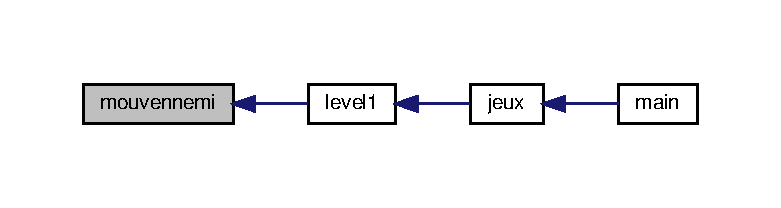
\includegraphics[width=350pt]{ennemi_8c_affe5e211a9cd4ecb89ed255a8f28e9f5_icgraph}
\end{center}
\end{figure}
\mbox{\Hypertarget{ennemi_8c_aebc98d93ce6c740a80cfe951a2303af9}\label{ennemi_8c_aebc98d93ce6c740a80cfe951a2303af9}} 
\index{ennemi.\+c@{ennemi.\+c}!splitennemi@{splitennemi}}
\index{splitennemi@{splitennemi}!ennemi.\+c@{ennemi.\+c}}
\subsubsection{\texorpdfstring{splitennemi()}{splitennemi()}}
{\footnotesize\ttfamily int splitennemi (\begin{DoxyParamCaption}\item[{int}]{y }\end{DoxyParamCaption})}

Here is the caller graph for this function\+:\nopagebreak
\begin{figure}[H]
\begin{center}
\leavevmode
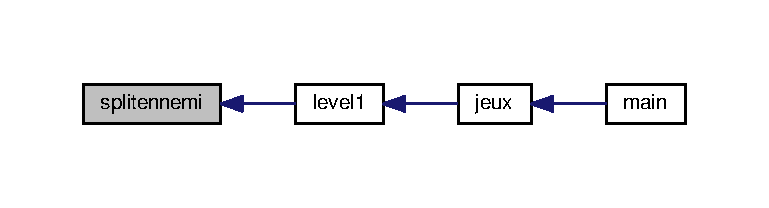
\includegraphics[width=350pt]{ennemi_8c_aebc98d93ce6c740a80cfe951a2303af9_icgraph}
\end{center}
\end{figure}

\hypertarget{ennemi_8h}{}\section{ennemi.\+h File Reference}
\label{ennemi_8h}\index{ennemi.\+h@{ennemi.\+h}}
This graph shows which files directly or indirectly include this file\+:\nopagebreak
\begin{figure}[H]
\begin{center}
\leavevmode
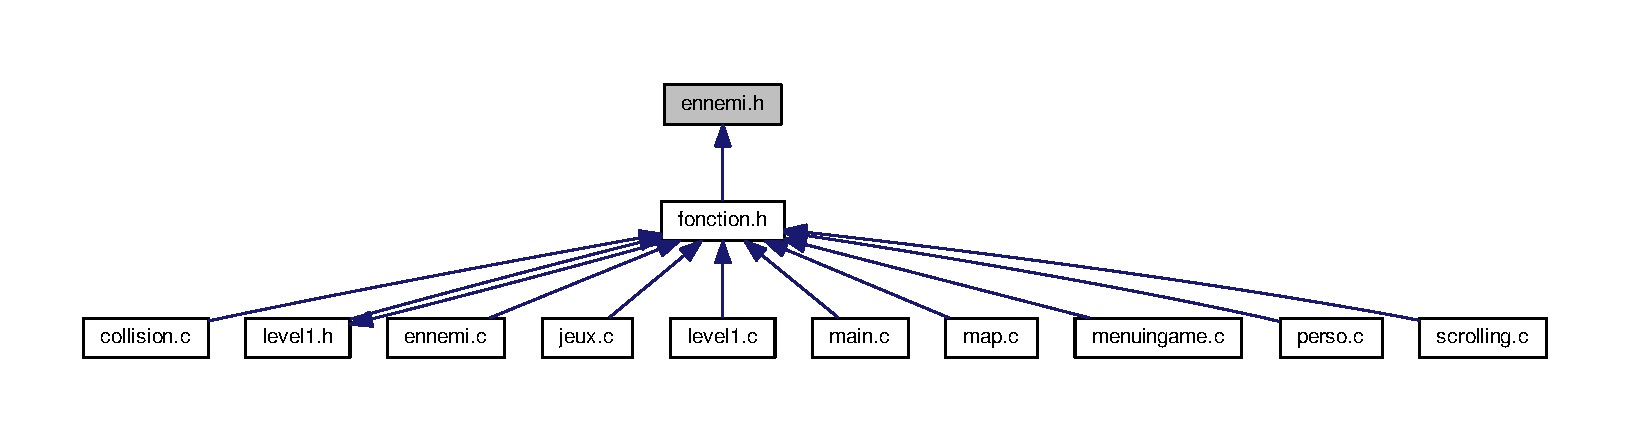
\includegraphics[width=350pt]{ennemi_8h__dep__incl}
\end{center}
\end{figure}
\subsection*{Data Structures}
\begin{DoxyCompactItemize}
\item 
struct \hyperlink{structennemis}{ennemis}
\end{DoxyCompactItemize}
\subsection*{Typedefs}
\begin{DoxyCompactItemize}
\item 
typedef struct \hyperlink{structennemis}{ennemis} \hyperlink{ennemi_8h_acd841d56b5672f28a310306985c7144b}{ennemis}
\end{DoxyCompactItemize}
\subsection*{Functions}
\begin{DoxyCompactItemize}
\item 
void \hyperlink{ennemi_8h_a7e97b6df5122a4ba309bff21a456dafa}{initialiserennemi} (\hyperlink{structennemis}{ennemis} $\ast$ennemi)
\item 
void \hyperlink{ennemi_8h_ac2414a6bd133a4ad2668dae5a823cdb3}{freesurfaceennemi} (\hyperlink{structennemis}{ennemis} $\ast$ennemi)
\item 
\hyperlink{structennemis}{ennemis} \hyperlink{ennemi_8h_affe5e211a9cd4ecb89ed255a8f28e9f5}{mouvennemi} (\hyperlink{structennemis}{ennemis} ennemi, \hyperlink{structperso}{perso} \hyperlink{structperso}{perso}, int d, int q, S\+D\+L\+\_\+\+Rect camera, S\+D\+L\+\_\+\+Surface $\ast$ecran, int $\ast$ennmouv, int $\ast$w, int $\ast$y, int mvmspeed)
\item 
int \hyperlink{ennemi_8h_aebc98d93ce6c740a80cfe951a2303af9}{splitennemi} (int y)
\item 
void \hyperlink{ennemi_8h_a3dc49b6654ac3b32977ce5ba4901c498}{afficherennemi} (\hyperlink{structennemis}{ennemis} ennemi, S\+D\+L\+\_\+\+Surface $\ast$ecran, int y)
\end{DoxyCompactItemize}


\subsection{Typedef Documentation}
\mbox{\Hypertarget{ennemi_8h_acd841d56b5672f28a310306985c7144b}\label{ennemi_8h_acd841d56b5672f28a310306985c7144b}} 
\index{ennemi.\+h@{ennemi.\+h}!ennemis@{ennemis}}
\index{ennemis@{ennemis}!ennemi.\+h@{ennemi.\+h}}
\subsubsection{\texorpdfstring{ennemis}{ennemis}}
{\footnotesize\ttfamily typedef struct \hyperlink{structennemis}{ennemis} \hyperlink{structennemis}{ennemis}}



\subsection{Function Documentation}
\mbox{\Hypertarget{ennemi_8h_a3dc49b6654ac3b32977ce5ba4901c498}\label{ennemi_8h_a3dc49b6654ac3b32977ce5ba4901c498}} 
\index{ennemi.\+h@{ennemi.\+h}!afficherennemi@{afficherennemi}}
\index{afficherennemi@{afficherennemi}!ennemi.\+h@{ennemi.\+h}}
\subsubsection{\texorpdfstring{afficherennemi()}{afficherennemi()}}
{\footnotesize\ttfamily void afficherennemi (\begin{DoxyParamCaption}\item[{\hyperlink{structennemis}{ennemis}}]{ennemi,  }\item[{S\+D\+L\+\_\+\+Surface $\ast$}]{ecran,  }\item[{int}]{y }\end{DoxyParamCaption})}

Here is the caller graph for this function\+:\nopagebreak
\begin{figure}[H]
\begin{center}
\leavevmode
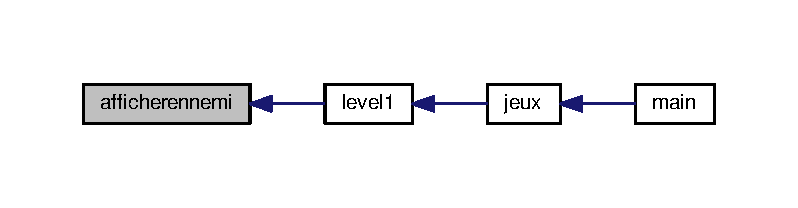
\includegraphics[width=350pt]{ennemi_8h_a3dc49b6654ac3b32977ce5ba4901c498_icgraph}
\end{center}
\end{figure}
\mbox{\Hypertarget{ennemi_8h_ac2414a6bd133a4ad2668dae5a823cdb3}\label{ennemi_8h_ac2414a6bd133a4ad2668dae5a823cdb3}} 
\index{ennemi.\+h@{ennemi.\+h}!freesurfaceennemi@{freesurfaceennemi}}
\index{freesurfaceennemi@{freesurfaceennemi}!ennemi.\+h@{ennemi.\+h}}
\subsubsection{\texorpdfstring{freesurfaceennemi()}{freesurfaceennemi()}}
{\footnotesize\ttfamily void freesurfaceennemi (\begin{DoxyParamCaption}\item[{\hyperlink{structennemis}{ennemis} $\ast$}]{ennemi }\end{DoxyParamCaption})}

Here is the caller graph for this function\+:\nopagebreak
\begin{figure}[H]
\begin{center}
\leavevmode
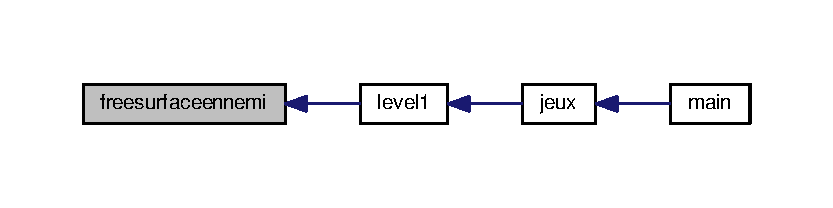
\includegraphics[width=350pt]{ennemi_8h_ac2414a6bd133a4ad2668dae5a823cdb3_icgraph}
\end{center}
\end{figure}
\mbox{\Hypertarget{ennemi_8h_a7e97b6df5122a4ba309bff21a456dafa}\label{ennemi_8h_a7e97b6df5122a4ba309bff21a456dafa}} 
\index{ennemi.\+h@{ennemi.\+h}!initialiserennemi@{initialiserennemi}}
\index{initialiserennemi@{initialiserennemi}!ennemi.\+h@{ennemi.\+h}}
\subsubsection{\texorpdfstring{initialiserennemi()}{initialiserennemi()}}
{\footnotesize\ttfamily void initialiserennemi (\begin{DoxyParamCaption}\item[{\hyperlink{structennemis}{ennemis} $\ast$}]{ennemi }\end{DoxyParamCaption})}

Here is the caller graph for this function\+:\nopagebreak
\begin{figure}[H]
\begin{center}
\leavevmode
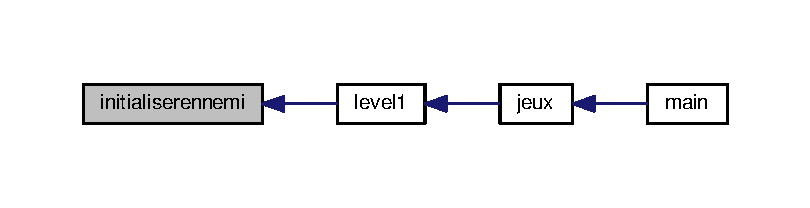
\includegraphics[width=350pt]{ennemi_8h_a7e97b6df5122a4ba309bff21a456dafa_icgraph}
\end{center}
\end{figure}
\mbox{\Hypertarget{ennemi_8h_affe5e211a9cd4ecb89ed255a8f28e9f5}\label{ennemi_8h_affe5e211a9cd4ecb89ed255a8f28e9f5}} 
\index{ennemi.\+h@{ennemi.\+h}!mouvennemi@{mouvennemi}}
\index{mouvennemi@{mouvennemi}!ennemi.\+h@{ennemi.\+h}}
\subsubsection{\texorpdfstring{mouvennemi()}{mouvennemi()}}
{\footnotesize\ttfamily \hyperlink{structennemis}{ennemis} mouvennemi (\begin{DoxyParamCaption}\item[{\hyperlink{structennemis}{ennemis}}]{ennemi,  }\item[{\hyperlink{structperso}{perso}}]{perso,  }\item[{int}]{d,  }\item[{int}]{q,  }\item[{S\+D\+L\+\_\+\+Rect}]{camera,  }\item[{S\+D\+L\+\_\+\+Surface $\ast$}]{ecran,  }\item[{int $\ast$}]{ennmouv,  }\item[{int $\ast$}]{w,  }\item[{int $\ast$}]{y,  }\item[{int}]{mvmspeed }\end{DoxyParamCaption})}

Here is the caller graph for this function\+:\nopagebreak
\begin{figure}[H]
\begin{center}
\leavevmode
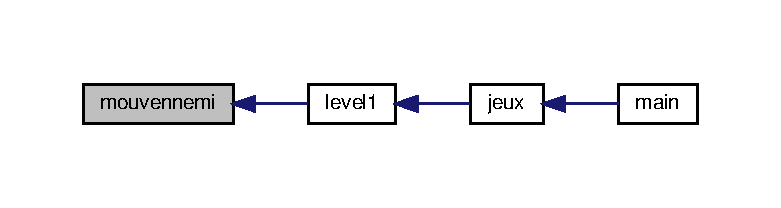
\includegraphics[width=350pt]{ennemi_8h_affe5e211a9cd4ecb89ed255a8f28e9f5_icgraph}
\end{center}
\end{figure}
\mbox{\Hypertarget{ennemi_8h_aebc98d93ce6c740a80cfe951a2303af9}\label{ennemi_8h_aebc98d93ce6c740a80cfe951a2303af9}} 
\index{ennemi.\+h@{ennemi.\+h}!splitennemi@{splitennemi}}
\index{splitennemi@{splitennemi}!ennemi.\+h@{ennemi.\+h}}
\subsubsection{\texorpdfstring{splitennemi()}{splitennemi()}}
{\footnotesize\ttfamily int splitennemi (\begin{DoxyParamCaption}\item[{int}]{y }\end{DoxyParamCaption})}

Here is the caller graph for this function\+:\nopagebreak
\begin{figure}[H]
\begin{center}
\leavevmode
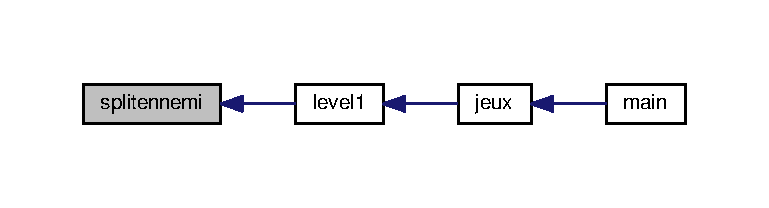
\includegraphics[width=350pt]{ennemi_8h_aebc98d93ce6c740a80cfe951a2303af9_icgraph}
\end{center}
\end{figure}

\hypertarget{fonction_8h}{}\section{fonction.\+h File Reference}
\label{fonction_8h}\index{fonction.\+h@{fonction.\+h}}
{\ttfamily \#include $<$stdio.\+h$>$}\newline
{\ttfamily \#include $<$S\+D\+L/\+S\+D\+L.\+h$>$}\newline
{\ttfamily \#include $<$S\+D\+L/\+S\+D\+L\+\_\+image.\+h$>$}\newline
{\ttfamily \#include $<$S\+D\+L/\+S\+D\+L\+\_\+mixer.\+h$>$}\newline
{\ttfamily \#include $<$time.\+h$>$}\newline
{\ttfamily \#include $<$unistd.\+h$>$}\newline
{\ttfamily \#include \char`\"{}jeux.\+h\char`\"{}}\newline
{\ttfamily \#include \char`\"{}map.\+h\char`\"{}}\newline
{\ttfamily \#include \char`\"{}perso.\+h\char`\"{}}\newline
{\ttfamily \#include \char`\"{}ennemi.\+h\char`\"{}}\newline
{\ttfamily \#include \char`\"{}collision.\+h\char`\"{}}\newline
{\ttfamily \#include \char`\"{}scrolling.\+h\char`\"{}}\newline
{\ttfamily \#include \char`\"{}menuingame.\+h\char`\"{}}\newline
{\ttfamily \#include \char`\"{}level1.\+h\char`\"{}}\newline
Include dependency graph for fonction.\+h\+:\nopagebreak
\begin{figure}[H]
\begin{center}
\leavevmode
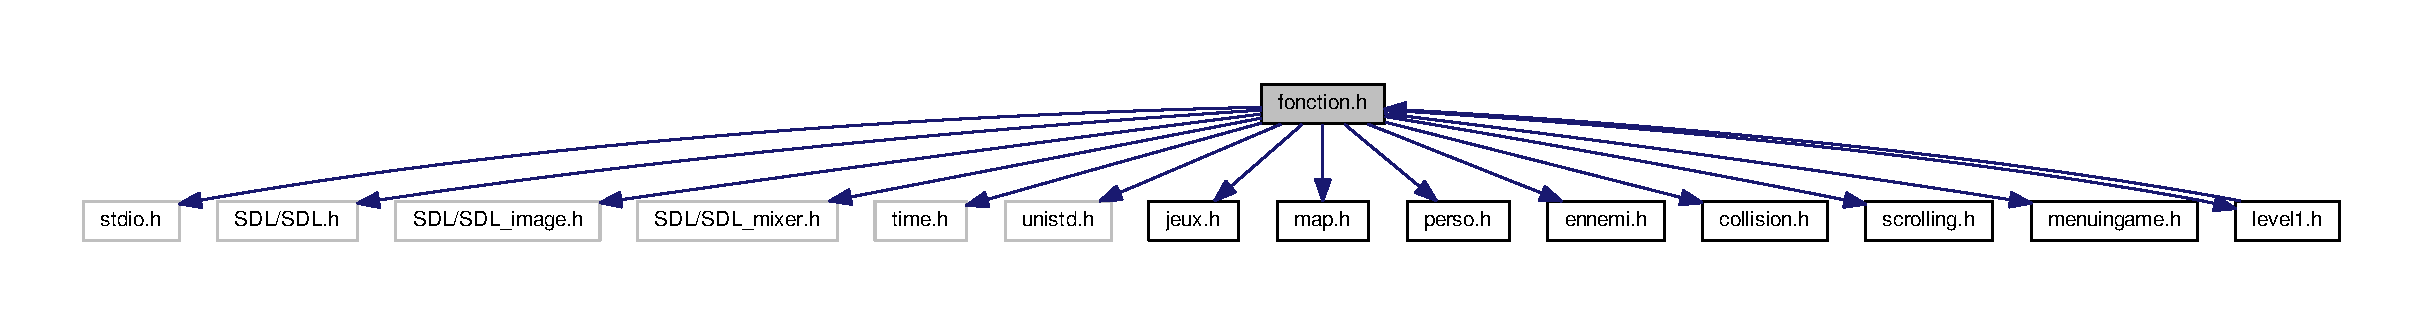
\includegraphics[width=350pt]{fonction_8h__incl}
\end{center}
\end{figure}
This graph shows which files directly or indirectly include this file\+:\nopagebreak
\begin{figure}[H]
\begin{center}
\leavevmode
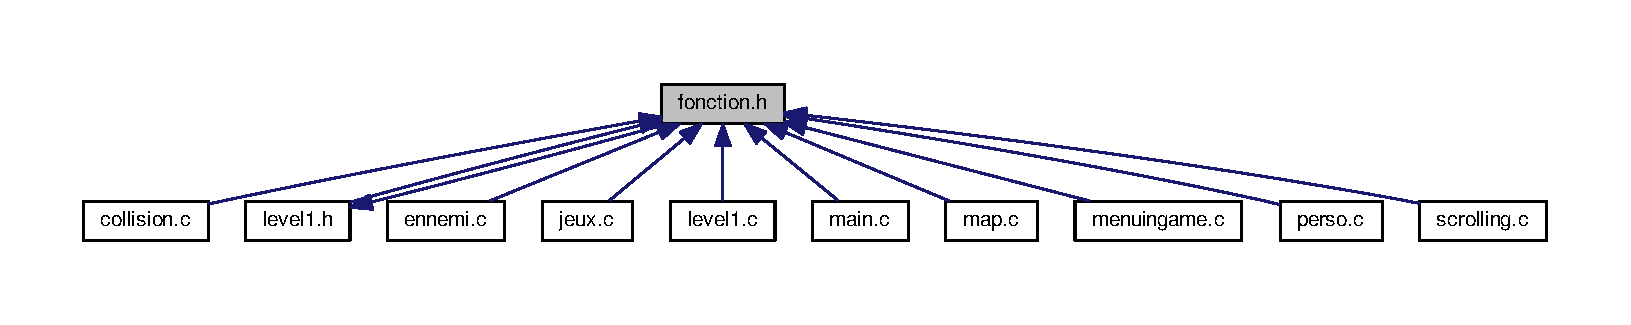
\includegraphics[width=350pt]{fonction_8h__dep__incl}
\end{center}
\end{figure}

\hypertarget{jeux_8c}{}\section{jeux.\+c File Reference}
\label{jeux_8c}\index{jeux.\+c@{jeux.\+c}}
{\ttfamily \#include \char`\"{}fonction.\+h\char`\"{}}\\*
Include dependency graph for jeux.\+c\+:
\nopagebreak
\begin{figure}[H]
\begin{center}
\leavevmode
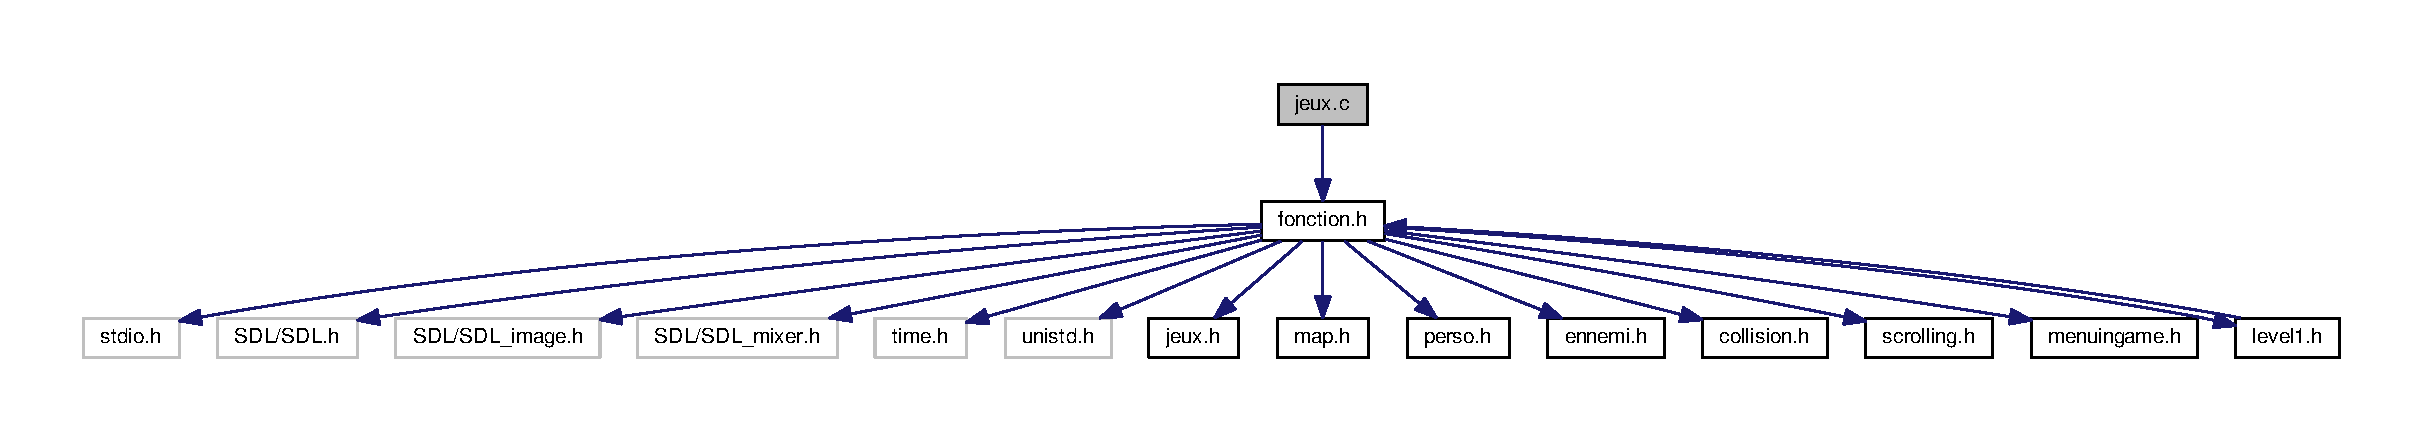
\includegraphics[width=350pt]{jeux_8c__incl}
\end{center}
\end{figure}
\subsection*{Functions}
\begin{DoxyCompactItemize}
\item 
void \hyperlink{jeux_8c_a63d2c3aa3cef693b94af238482276255}{jeux} (int lvl)
\end{DoxyCompactItemize}


\subsection{Function Documentation}
\index{jeux.\+c@{jeux.\+c}!jeux@{jeux}}
\index{jeux@{jeux}!jeux.\+c@{jeux.\+c}}
\subsubsection[{\texorpdfstring{jeux(int lvl)}{jeux(int lvl)}}]{\setlength{\rightskip}{0pt plus 5cm}void jeux (
\begin{DoxyParamCaption}
\item[{int}]{lvl}
\end{DoxyParamCaption}
)}\hypertarget{jeux_8c_a63d2c3aa3cef693b94af238482276255}{}\label{jeux_8c_a63d2c3aa3cef693b94af238482276255}


Here is the call graph for this function\+:
\nopagebreak
\begin{figure}[H]
\begin{center}
\leavevmode
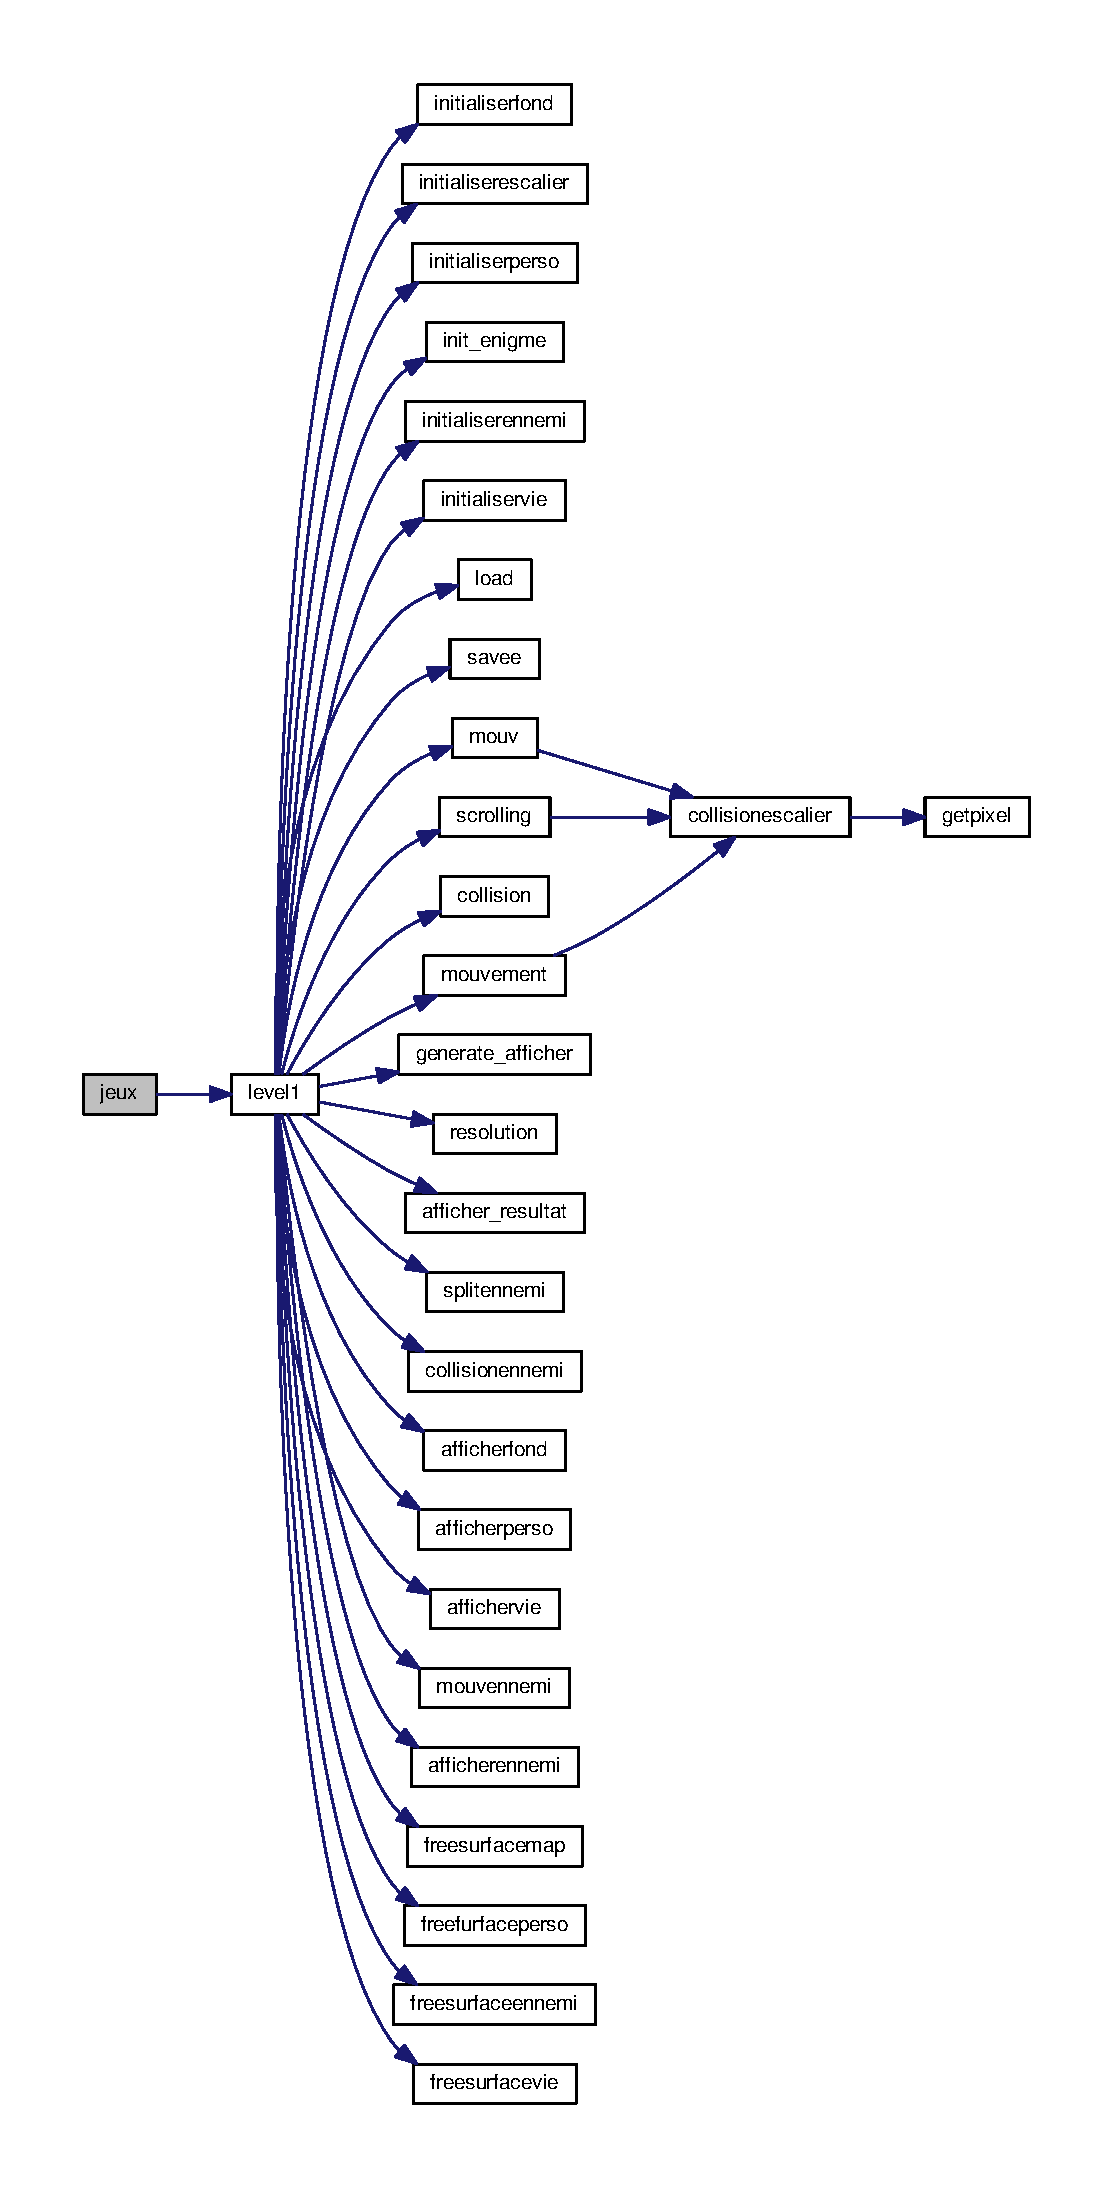
\includegraphics[height=550pt]{jeux_8c_a63d2c3aa3cef693b94af238482276255_cgraph}
\end{center}
\end{figure}




Here is the caller graph for this function\+:
\nopagebreak
\begin{figure}[H]
\begin{center}
\leavevmode
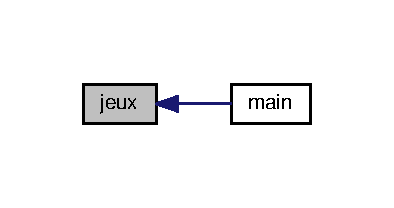
\includegraphics[width=189pt]{jeux_8c_a63d2c3aa3cef693b94af238482276255_icgraph}
\end{center}
\end{figure}



\hypertarget{jeux_8h}{}\section{jeux.\+h File Reference}
\label{jeux_8h}\index{jeux.\+h@{jeux.\+h}}
This graph shows which files directly or indirectly include this file\+:\nopagebreak
\begin{figure}[H]
\begin{center}
\leavevmode
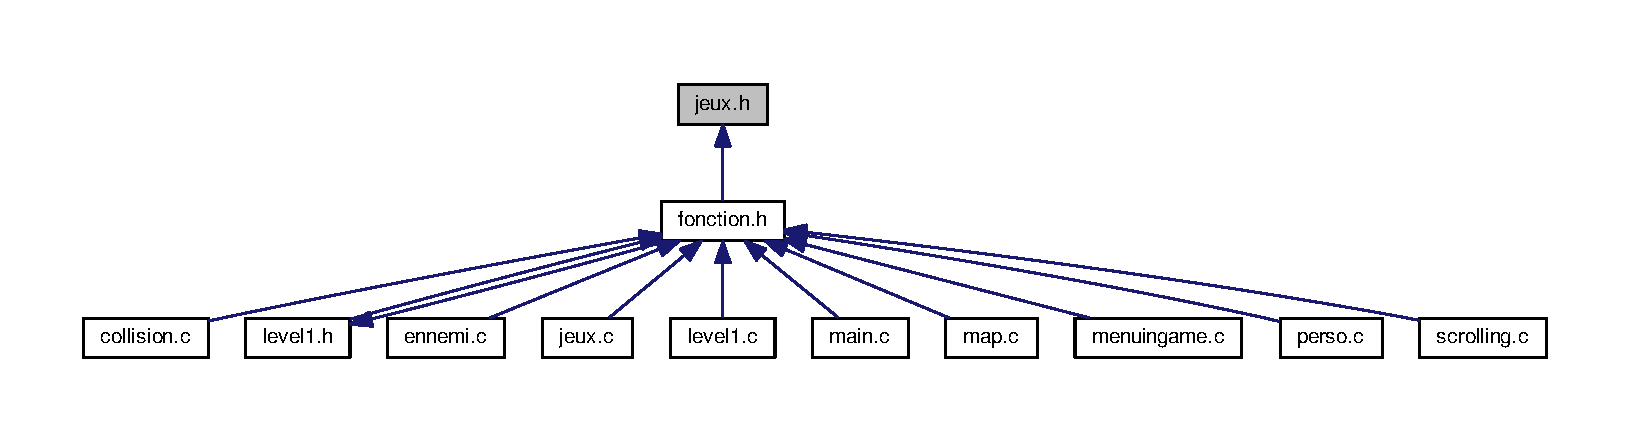
\includegraphics[width=350pt]{jeux_8h__dep__incl}
\end{center}
\end{figure}
\subsection*{Functions}
\begin{DoxyCompactItemize}
\item 
void \hyperlink{jeux_8h_ad38cf6359c3f38f66e6aa46a96ecc347}{jeux} (int save)
\end{DoxyCompactItemize}


\subsection{Function Documentation}
\mbox{\Hypertarget{jeux_8h_ad38cf6359c3f38f66e6aa46a96ecc347}\label{jeux_8h_ad38cf6359c3f38f66e6aa46a96ecc347}} 
\index{jeux.\+h@{jeux.\+h}!jeux@{jeux}}
\index{jeux@{jeux}!jeux.\+h@{jeux.\+h}}
\subsubsection{\texorpdfstring{jeux()}{jeux()}}
{\footnotesize\ttfamily void jeux (\begin{DoxyParamCaption}\item[{int}]{save }\end{DoxyParamCaption})}

Here is the call graph for this function\+:\nopagebreak
\begin{figure}[H]
\begin{center}
\leavevmode
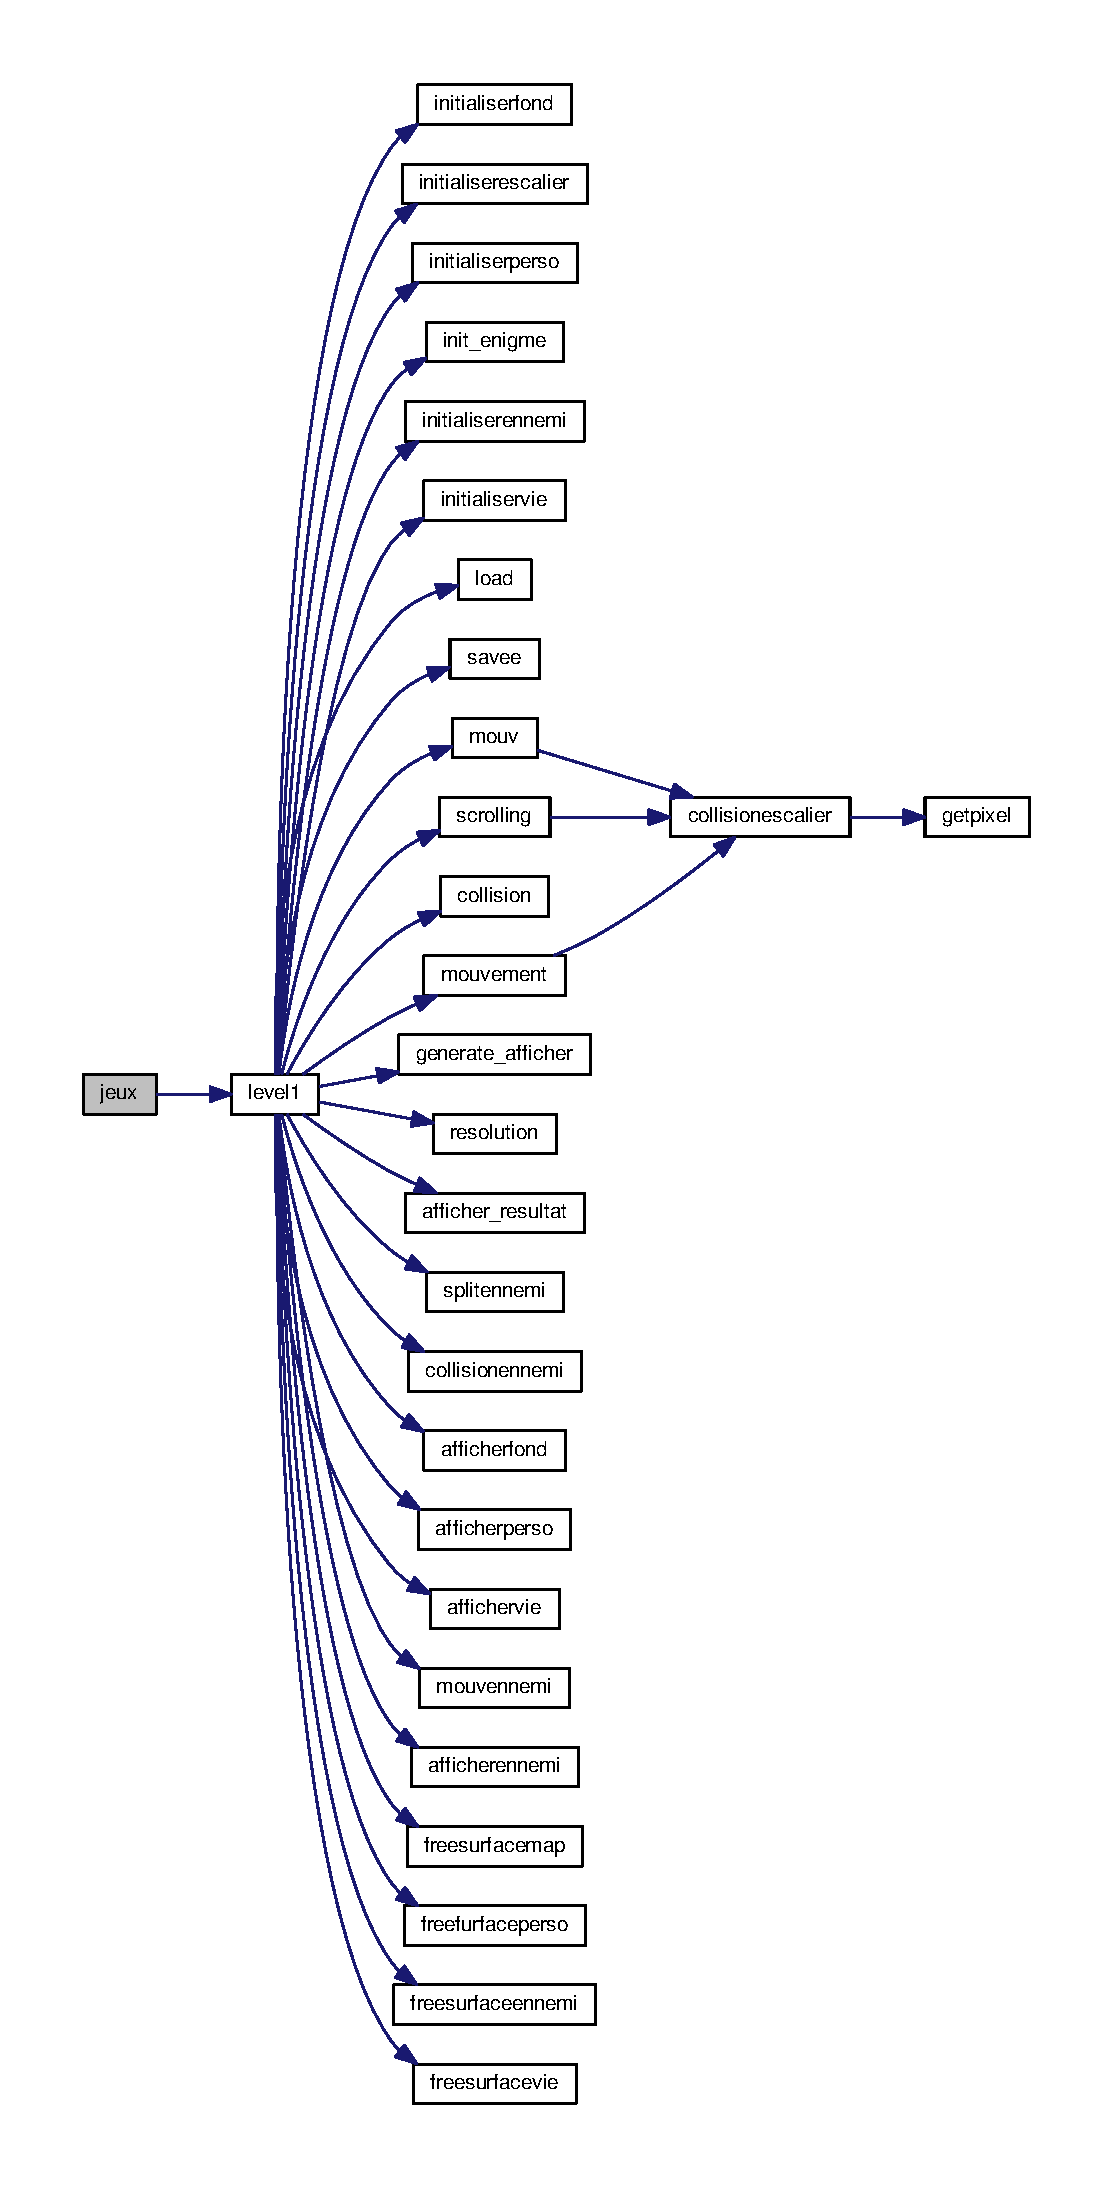
\includegraphics[height=550pt]{jeux_8h_ad38cf6359c3f38f66e6aa46a96ecc347_cgraph}
\end{center}
\end{figure}
Here is the caller graph for this function\+:\nopagebreak
\begin{figure}[H]
\begin{center}
\leavevmode
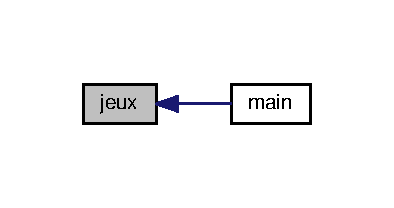
\includegraphics[width=189pt]{jeux_8h_ad38cf6359c3f38f66e6aa46a96ecc347_icgraph}
\end{center}
\end{figure}

\hypertarget{level1_8c}{}\section{level1.\+c File Reference}
\label{level1_8c}\index{level1.\+c@{level1.\+c}}
{\ttfamily \#include \char`\"{}fonction.\+h\char`\"{}}\newline
{\ttfamily \#include \char`\"{}enigme.\+h\char`\"{}}\newline
Include dependency graph for level1.\+c\+:\nopagebreak
\begin{figure}[H]
\begin{center}
\leavevmode
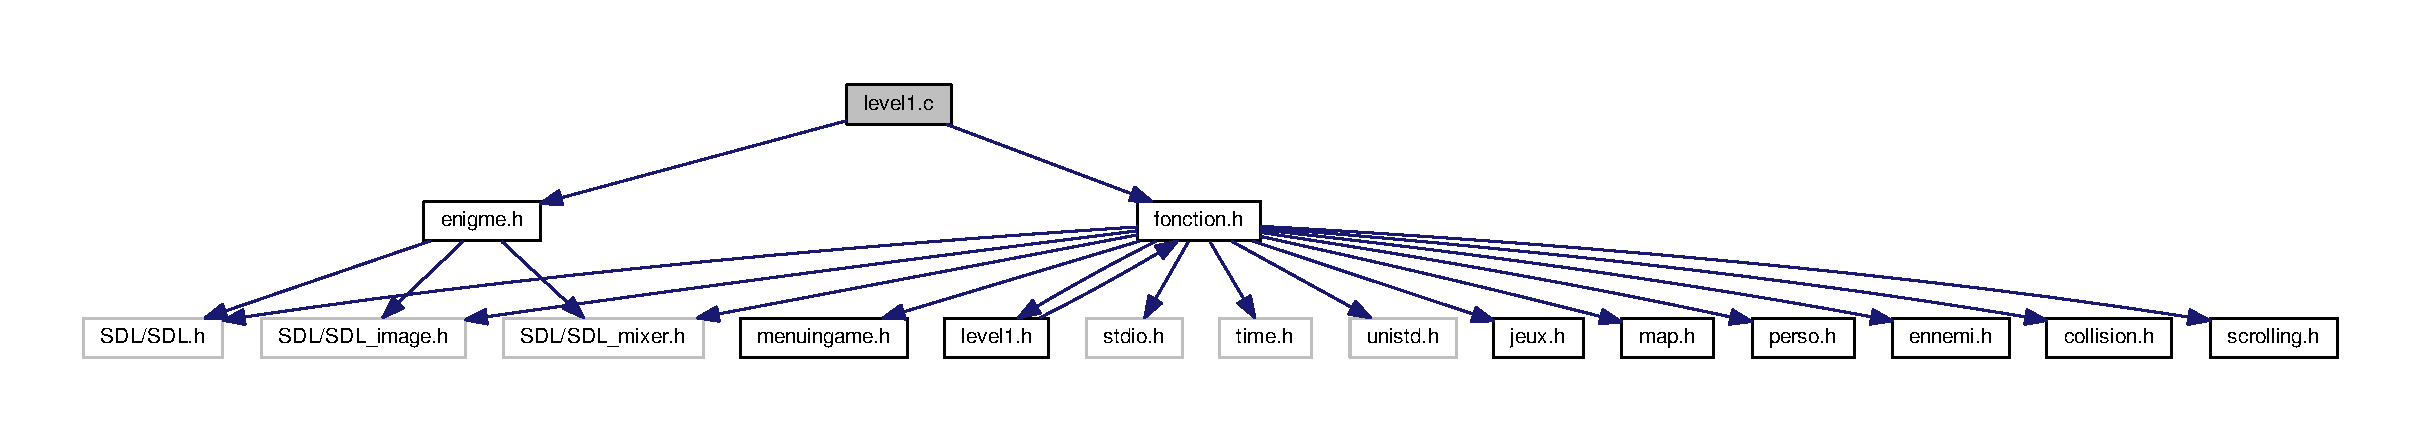
\includegraphics[width=350pt]{level1_8c__incl}
\end{center}
\end{figure}
\subsection*{Functions}
\begin{DoxyCompactItemize}
\item 
void \hyperlink{level1_8c_a22a96d4675403385bc77052267e5f4e7}{savee} (\hyperlink{structennemis}{ennemis} ennemi, \hyperlink{structperso}{perso} \hyperlink{structperso}{perso}, int page1, int page2, \hyperlink{structvie}{vie} \hyperlink{structvie}{vie}, int saut, S\+D\+L\+\_\+\+Rect camera)
\item 
void \hyperlink{level1_8c_a597cdfe56a6e01445add67a881570581}{load} (int lvl, \hyperlink{structennemis}{ennemis} $\ast$ennemi, \hyperlink{structperso}{perso} $\ast$\hyperlink{structperso}{perso}, int page1, int page2, \hyperlink{structvie}{vie} $\ast$\hyperlink{structvie}{vie}, int $\ast$saut, S\+D\+L\+\_\+\+Rect $\ast$camera, int $\ast$continuer, int $\ast$save)
\item 
void \hyperlink{level1_8c_afd6b3dbc219eac712d9b2075aea92cba}{level1} (int $\ast$save, int lvl)
\end{DoxyCompactItemize}


\subsection{Function Documentation}
\mbox{\Hypertarget{level1_8c_afd6b3dbc219eac712d9b2075aea92cba}\label{level1_8c_afd6b3dbc219eac712d9b2075aea92cba}} 
\index{level1.\+c@{level1.\+c}!level1@{level1}}
\index{level1@{level1}!level1.\+c@{level1.\+c}}
\subsubsection{\texorpdfstring{level1()}{level1()}}
{\footnotesize\ttfamily void level1 (\begin{DoxyParamCaption}\item[{int $\ast$}]{save,  }\item[{int}]{lvl }\end{DoxyParamCaption})}

init\+\_\+enigme(\&enig); Here is the call graph for this function\+:\nopagebreak
\begin{figure}[H]
\begin{center}
\leavevmode
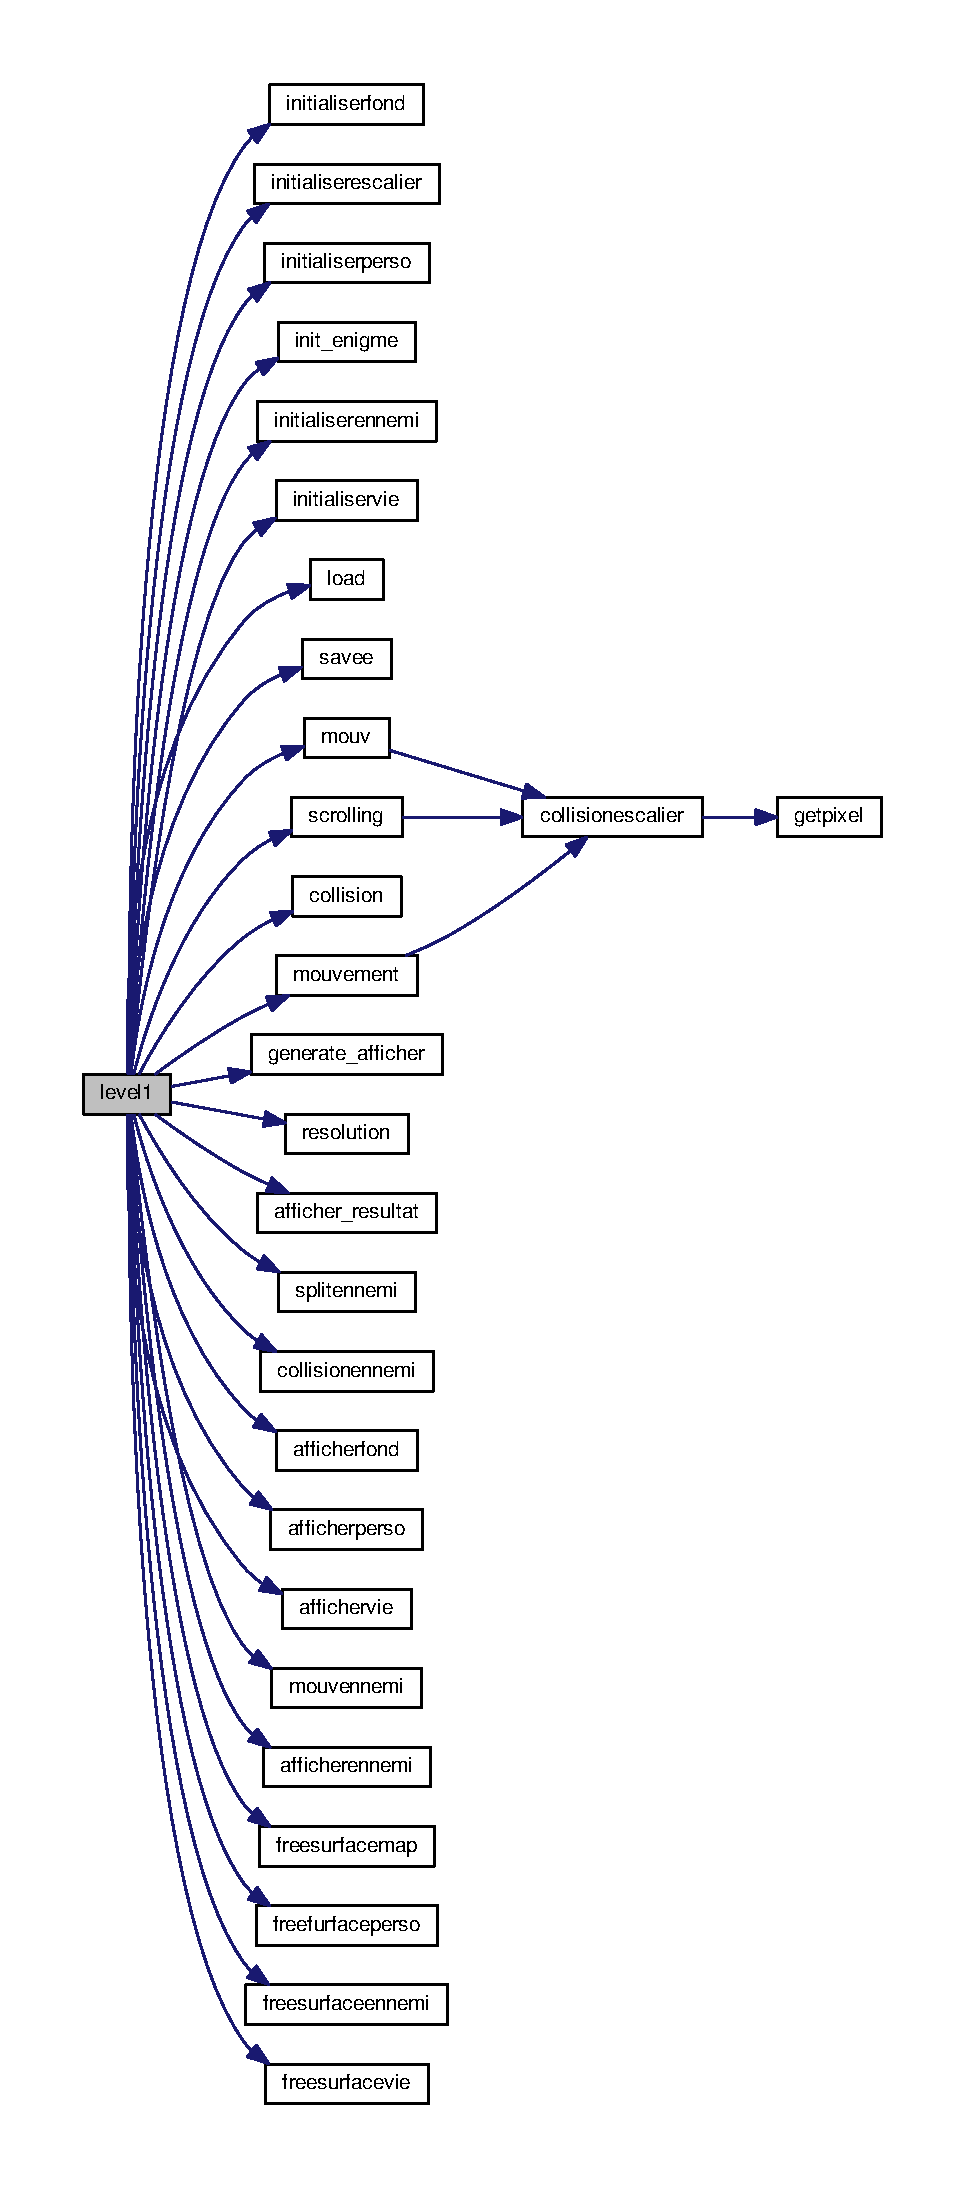
\includegraphics[height=550pt]{level1_8c_afd6b3dbc219eac712d9b2075aea92cba_cgraph}
\end{center}
\end{figure}
Here is the caller graph for this function\+:\nopagebreak
\begin{figure}[H]
\begin{center}
\leavevmode
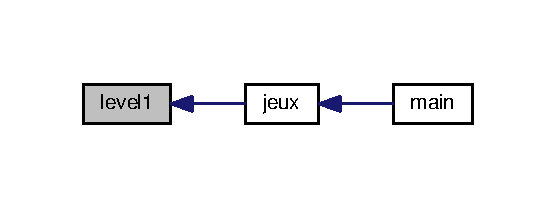
\includegraphics[width=267pt]{level1_8c_afd6b3dbc219eac712d9b2075aea92cba_icgraph}
\end{center}
\end{figure}
\mbox{\Hypertarget{level1_8c_a597cdfe56a6e01445add67a881570581}\label{level1_8c_a597cdfe56a6e01445add67a881570581}} 
\index{level1.\+c@{level1.\+c}!load@{load}}
\index{load@{load}!level1.\+c@{level1.\+c}}
\subsubsection{\texorpdfstring{load()}{load()}}
{\footnotesize\ttfamily void load (\begin{DoxyParamCaption}\item[{int}]{lvl,  }\item[{\hyperlink{structennemis}{ennemis} $\ast$}]{ennemi,  }\item[{\hyperlink{structperso}{perso} $\ast$}]{perso,  }\item[{int}]{page1,  }\item[{int}]{page2,  }\item[{\hyperlink{structvie}{vie} $\ast$}]{vie,  }\item[{int $\ast$}]{saut,  }\item[{S\+D\+L\+\_\+\+Rect $\ast$}]{camera,  }\item[{int $\ast$}]{continuer,  }\item[{int $\ast$}]{save }\end{DoxyParamCaption})}

Here is the caller graph for this function\+:\nopagebreak
\begin{figure}[H]
\begin{center}
\leavevmode
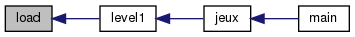
\includegraphics[width=338pt]{level1_8c_a597cdfe56a6e01445add67a881570581_icgraph}
\end{center}
\end{figure}
\mbox{\Hypertarget{level1_8c_a22a96d4675403385bc77052267e5f4e7}\label{level1_8c_a22a96d4675403385bc77052267e5f4e7}} 
\index{level1.\+c@{level1.\+c}!savee@{savee}}
\index{savee@{savee}!level1.\+c@{level1.\+c}}
\subsubsection{\texorpdfstring{savee()}{savee()}}
{\footnotesize\ttfamily void savee (\begin{DoxyParamCaption}\item[{\hyperlink{structennemis}{ennemis}}]{ennemi,  }\item[{\hyperlink{structperso}{perso}}]{perso,  }\item[{int}]{page1,  }\item[{int}]{page2,  }\item[{\hyperlink{structvie}{vie}}]{vie,  }\item[{int}]{saut,  }\item[{S\+D\+L\+\_\+\+Rect}]{camera }\end{DoxyParamCaption})}

Here is the caller graph for this function\+:\nopagebreak
\begin{figure}[H]
\begin{center}
\leavevmode
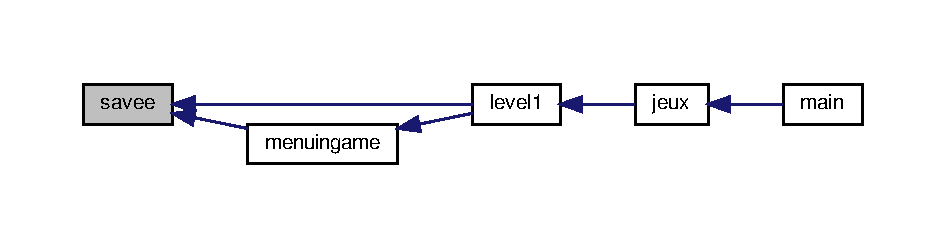
\includegraphics[width=350pt]{level1_8c_a22a96d4675403385bc77052267e5f4e7_icgraph}
\end{center}
\end{figure}

\hypertarget{level1_8h}{}\section{level1.\+h File Reference}
\label{level1_8h}\index{level1.\+h@{level1.\+h}}
{\ttfamily \#include \char`\"{}fonction.\+h\char`\"{}}\\*
Include dependency graph for level1.\+h\+:
\nopagebreak
\begin{figure}[H]
\begin{center}
\leavevmode
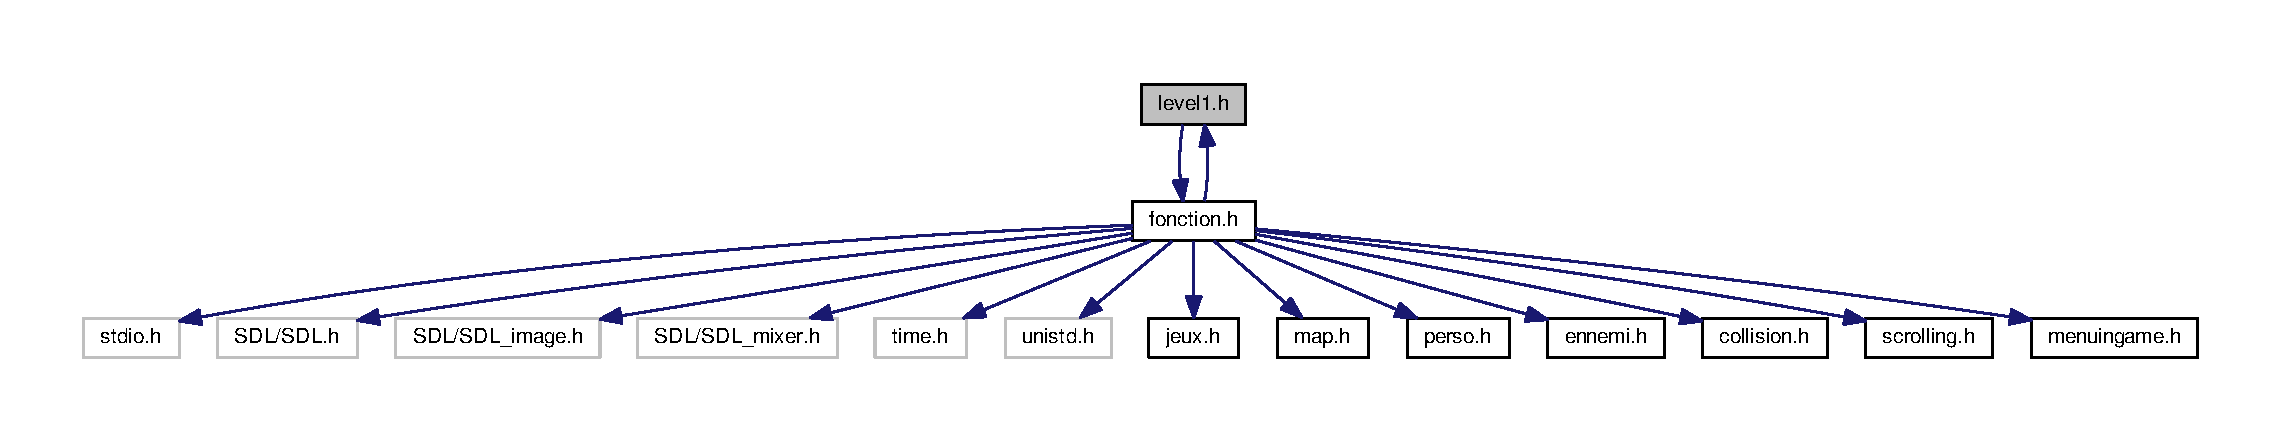
\includegraphics[width=350pt]{level1_8h__incl}
\end{center}
\end{figure}
This graph shows which files directly or indirectly include this file\+:
\nopagebreak
\begin{figure}[H]
\begin{center}
\leavevmode
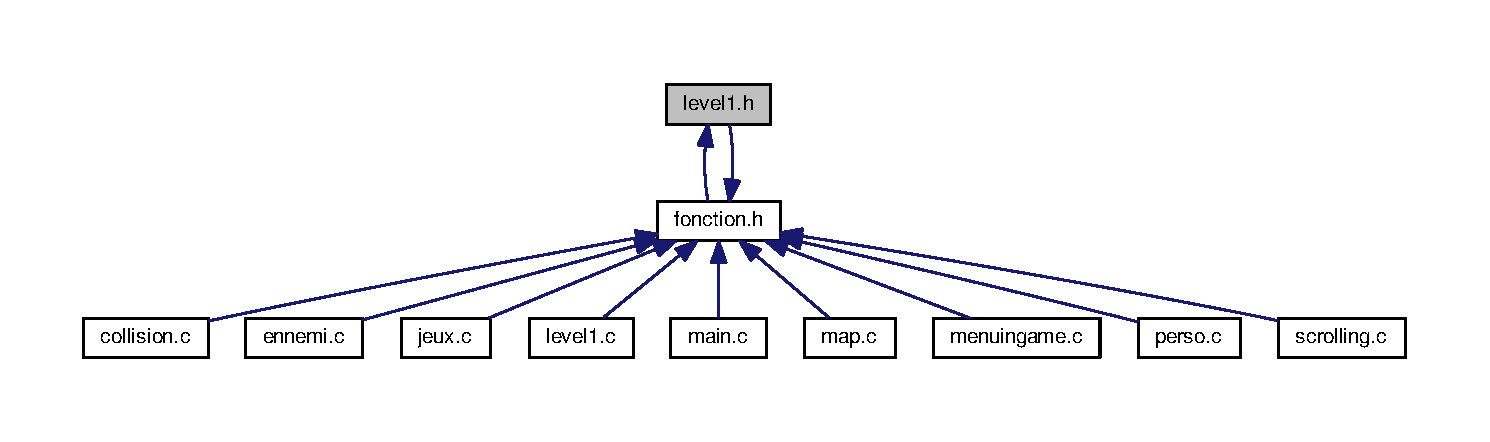
\includegraphics[width=350pt]{level1_8h__dep__incl}
\end{center}
\end{figure}
\subsection*{Data Structures}
\begin{DoxyCompactItemize}
\item 
struct \hyperlink{structsaves}{saves}
\end{DoxyCompactItemize}
\subsection*{Typedefs}
\begin{DoxyCompactItemize}
\item 
typedef struct \hyperlink{structsaves}{saves} \hyperlink{level1_8h_af90c8fac7a7f8d54e56773454147bab2}{saves}
\end{DoxyCompactItemize}
\subsection*{Functions}
\begin{DoxyCompactItemize}
\item 
void \hyperlink{level1_8h_a29092ba4fe09a81f884fc05a61498891}{savee} (\hyperlink{structennemis}{ennemis} ennemi, \hyperlink{structperso}{perso} \hyperlink{structperso}{perso}, \hyperlink{structvie}{vie} \hyperlink{structvie}{vie}, int saut, S\+D\+L\+\_\+\+Rect camera)
\item 
void \hyperlink{level1_8h_a4b08faa6aa2777a535b1db0b48669e0e}{load} (int lvl, \hyperlink{structennemis}{ennemis} $\ast$ennemi, \hyperlink{structperso}{perso} $\ast$\hyperlink{structperso}{perso}, \hyperlink{structvie}{vie} $\ast$\hyperlink{structvie}{vie}, int $\ast$saut, S\+D\+L\+\_\+\+Rect $\ast$camera, int $\ast$continuer, int $\ast$save)
\item 
void \hyperlink{level1_8h_afd6b3dbc219eac712d9b2075aea92cba}{level1} (int $\ast$save, int lvl)
\end{DoxyCompactItemize}


\subsection{Typedef Documentation}
\index{level1.\+h@{level1.\+h}!saves@{saves}}
\index{saves@{saves}!level1.\+h@{level1.\+h}}
\subsubsection[{\texorpdfstring{saves}{saves}}]{\setlength{\rightskip}{0pt plus 5cm}typedef struct {\bf saves} {\bf saves}}\hypertarget{level1_8h_af90c8fac7a7f8d54e56773454147bab2}{}\label{level1_8h_af90c8fac7a7f8d54e56773454147bab2}


\subsection{Function Documentation}
\index{level1.\+h@{level1.\+h}!level1@{level1}}
\index{level1@{level1}!level1.\+h@{level1.\+h}}
\subsubsection[{\texorpdfstring{level1(int $\ast$save, int lvl)}{level1(int *save, int lvl)}}]{\setlength{\rightskip}{0pt plus 5cm}void level1 (
\begin{DoxyParamCaption}
\item[{int $\ast$}]{save, }
\item[{int}]{lvl}
\end{DoxyParamCaption}
)}\hypertarget{level1_8h_afd6b3dbc219eac712d9b2075aea92cba}{}\label{level1_8h_afd6b3dbc219eac712d9b2075aea92cba}


Here is the call graph for this function\+:
\nopagebreak
\begin{figure}[H]
\begin{center}
\leavevmode
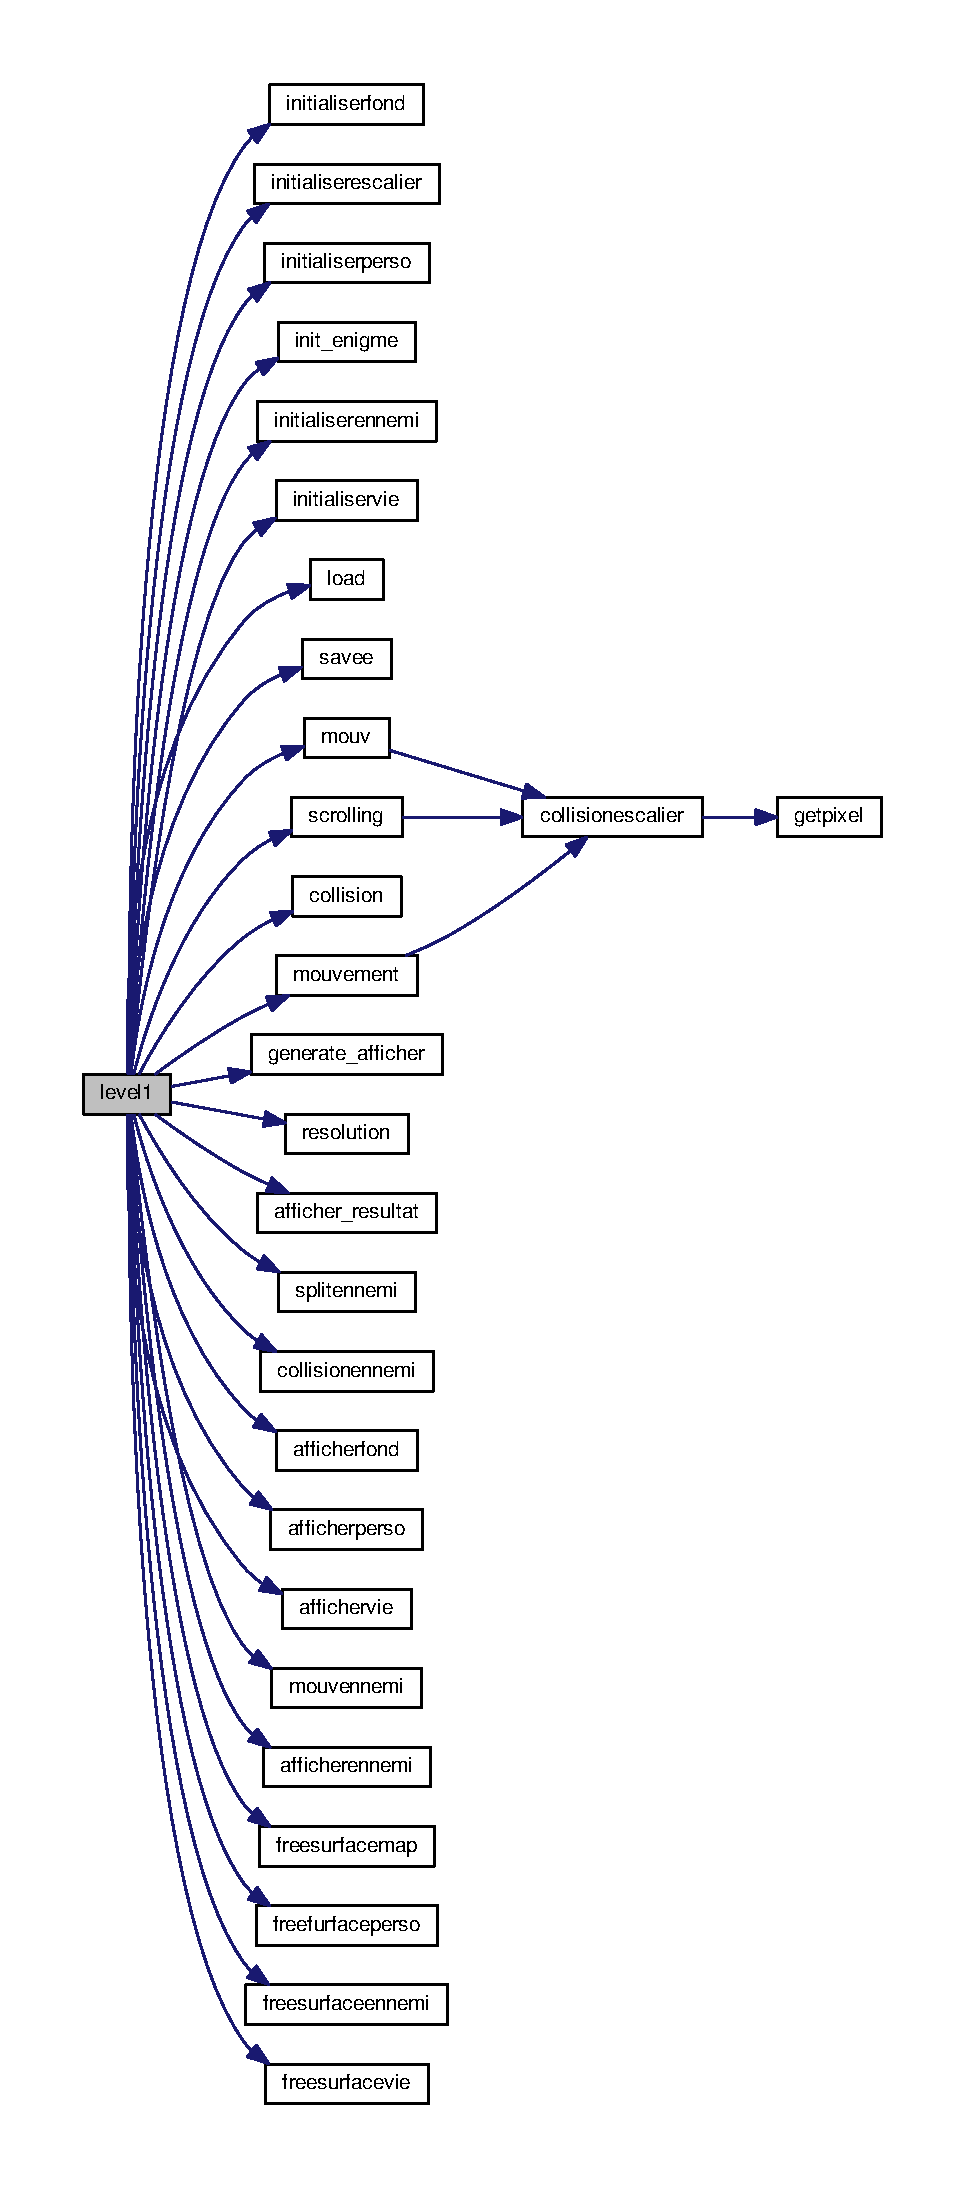
\includegraphics[height=550pt]{level1_8h_afd6b3dbc219eac712d9b2075aea92cba_cgraph}
\end{center}
\end{figure}




Here is the caller graph for this function\+:
\nopagebreak
\begin{figure}[H]
\begin{center}
\leavevmode
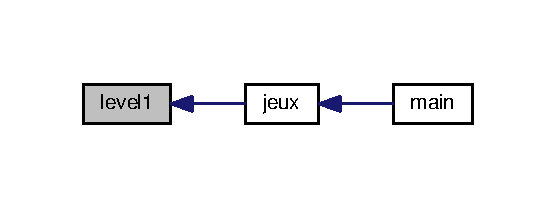
\includegraphics[width=267pt]{level1_8h_afd6b3dbc219eac712d9b2075aea92cba_icgraph}
\end{center}
\end{figure}


\index{level1.\+h@{level1.\+h}!load@{load}}
\index{load@{load}!level1.\+h@{level1.\+h}}
\subsubsection[{\texorpdfstring{load(int lvl, ennemis $\ast$ennemi, perso $\ast$perso, vie $\ast$vie, int $\ast$saut, S\+D\+L\+\_\+\+Rect $\ast$camera, int $\ast$continuer, int $\ast$save)}{load(int lvl, ennemis *ennemi, perso *perso, vie *vie, int *saut, SDL_Rect *camera, int *continuer, int *save)}}]{\setlength{\rightskip}{0pt plus 5cm}void load (
\begin{DoxyParamCaption}
\item[{int}]{lvl, }
\item[{{\bf ennemis} $\ast$}]{ennemi, }
\item[{{\bf perso} $\ast$}]{perso, }
\item[{{\bf vie} $\ast$}]{vie, }
\item[{int $\ast$}]{saut, }
\item[{S\+D\+L\+\_\+\+Rect $\ast$}]{camera, }
\item[{int $\ast$}]{continuer, }
\item[{int $\ast$}]{save}
\end{DoxyParamCaption}
)}\hypertarget{level1_8h_a4b08faa6aa2777a535b1db0b48669e0e}{}\label{level1_8h_a4b08faa6aa2777a535b1db0b48669e0e}


Here is the caller graph for this function\+:
\nopagebreak
\begin{figure}[H]
\begin{center}
\leavevmode
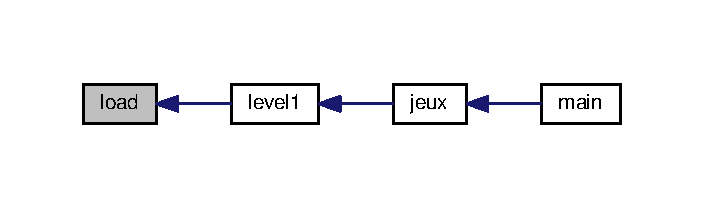
\includegraphics[width=338pt]{level1_8h_a4b08faa6aa2777a535b1db0b48669e0e_icgraph}
\end{center}
\end{figure}


\index{level1.\+h@{level1.\+h}!savee@{savee}}
\index{savee@{savee}!level1.\+h@{level1.\+h}}
\subsubsection[{\texorpdfstring{savee(ennemis ennemi, perso perso, vie vie, int saut, S\+D\+L\+\_\+\+Rect camera)}{savee(ennemis ennemi, perso perso, vie vie, int saut, SDL_Rect camera)}}]{\setlength{\rightskip}{0pt plus 5cm}void savee (
\begin{DoxyParamCaption}
\item[{{\bf ennemis}}]{ennemi, }
\item[{{\bf perso}}]{perso, }
\item[{{\bf vie}}]{vie, }
\item[{int}]{saut, }
\item[{S\+D\+L\+\_\+\+Rect}]{camera}
\end{DoxyParamCaption}
)}\hypertarget{level1_8h_a29092ba4fe09a81f884fc05a61498891}{}\label{level1_8h_a29092ba4fe09a81f884fc05a61498891}


Here is the caller graph for this function\+:
\nopagebreak
\begin{figure}[H]
\begin{center}
\leavevmode
\includegraphics[width=350pt]{level1_8h_a29092ba4fe09a81f884fc05a61498891_icgraph}
\end{center}
\end{figure}



\hypertarget{main_8c}{}\section{main.\+c File Reference}
\label{main_8c}\index{main.\+c@{main.\+c}}
{\ttfamily \#include \char`\"{}fonction.\+h\char`\"{}}\newline
Include dependency graph for main.\+c\+:\nopagebreak
\begin{figure}[H]
\begin{center}
\leavevmode
\includegraphics[width=350pt]{main_8c__incl}
\end{center}
\end{figure}
\subsection*{Functions}
\begin{DoxyCompactItemize}
\item 
int \hyperlink{main_8c_a0ddf1224851353fc92bfbff6f499fa97}{main} (int argc, char $\ast$argv\mbox{[}$\,$\mbox{]})
\end{DoxyCompactItemize}


\subsection{Function Documentation}
\mbox{\Hypertarget{main_8c_a0ddf1224851353fc92bfbff6f499fa97}\label{main_8c_a0ddf1224851353fc92bfbff6f499fa97}} 
\index{main.\+c@{main.\+c}!main@{main}}
\index{main@{main}!main.\+c@{main.\+c}}
\subsubsection{\texorpdfstring{main()}{main()}}
{\footnotesize\ttfamily int main (\begin{DoxyParamCaption}\item[{int}]{argc,  }\item[{char $\ast$}]{argv\mbox{[}$\,$\mbox{]} }\end{DoxyParamCaption})}

Here is the call graph for this function\+:\nopagebreak
\begin{figure}[H]
\begin{center}
\leavevmode
\includegraphics[width=350pt]{main_8c_a0ddf1224851353fc92bfbff6f499fa97_cgraph}
\end{center}
\end{figure}

\hypertarget{map_8c}{}\section{map.\+c File Reference}
\label{map_8c}\index{map.\+c@{map.\+c}}
{\ttfamily \#include \char`\"{}fonction.\+h\char`\"{}}\newline
Include dependency graph for map.\+c\+:\nopagebreak
\begin{figure}[H]
\begin{center}
\leavevmode
\includegraphics[width=350pt]{map_8c__incl}
\end{center}
\end{figure}
\subsection*{Functions}
\begin{DoxyCompactItemize}
\item 
void \hyperlink{map_8c_a4064b8904eab2845f682ad0e607a49c8}{initialiserfond} (\hyperlink{structmap}{map} $\ast$\hyperlink{structmap}{map})
\begin{DoxyCompactList}\small\item\em To initialize the background map . \end{DoxyCompactList}\item 
$\ast$void \hyperlink{map_8c_a1e8147ba3e5ef420d319afcfa0f67185}{initialiserfond2} (\hyperlink{structmap}{map} $\ast$\hyperlink{structmap}{map})
\begin{DoxyCompactList}\small\item\em To initialize the background map . \end{DoxyCompactList}\item 
$\ast$void \hyperlink{map_8c_aa895744df6e1498922783d1711b017ec}{initialiserfond3} (\hyperlink{structmap}{map} $\ast$\hyperlink{structmap}{map})
\begin{DoxyCompactList}\small\item\em To initialize the background map . \end{DoxyCompactList}\item 
$\ast$void \hyperlink{map_8c_a1092d4a65fa3d0d880a8133f7c164a7c}{initialiserescalier} (\hyperlink{structescalier}{escalier} $\ast$\hyperlink{structescalier}{escalier})
\begin{DoxyCompactList}\small\item\em To initialize escalier . \end{DoxyCompactList}\item 
$\ast$void \hyperlink{map_8c_addb79ce7d8cd64cc5d5c4c29e3bbae23}{freesurfacemap} (\hyperlink{structmap}{map} $\ast$\hyperlink{structmap}{map}, \hyperlink{structescalier}{escalier} $\ast$\hyperlink{structescalier}{escalier})
\begin{DoxyCompactList}\small\item\em To free the background map and escalier . \end{DoxyCompactList}\item 
$\ast$void \hyperlink{map_8c_a16c367d2cc7f5831c7b03e1bb5edb8f9}{afficherfond} (\hyperlink{structmap}{map} \hyperlink{structmap}{map}, S\+D\+L\+\_\+\+Rect $\ast$camera, S\+D\+L\+\_\+\+Surface $\ast$ecran)
\begin{DoxyCompactList}\small\item\em To show the background map . \end{DoxyCompactList}\end{DoxyCompactItemize}


\subsection{Function Documentation}
\mbox{\Hypertarget{map_8c_a16c367d2cc7f5831c7b03e1bb5edb8f9}\label{map_8c_a16c367d2cc7f5831c7b03e1bb5edb8f9}} 
\index{map.\+c@{map.\+c}!afficherfond@{afficherfond}}
\index{afficherfond@{afficherfond}!map.\+c@{map.\+c}}
\subsubsection{\texorpdfstring{afficherfond()}{afficherfond()}}
{\footnotesize\ttfamily $\ast$ void afficherfond (\begin{DoxyParamCaption}\item[{\hyperlink{structmap}{map}}]{map,  }\item[{S\+D\+L\+\_\+\+Rect $\ast$}]{camera,  }\item[{S\+D\+L\+\_\+\+Surface $\ast$}]{ecran }\end{DoxyParamCaption})}



To show the background map . 


\begin{DoxyParams}{Parameters}
{\em map} & the background \\
\hline
{\em camera} & \\
\hline
{\em ecran} & (the screen) \\
\hline
\end{DoxyParams}
\begin{DoxyReturn}{Returns}
Nothing 
\end{DoxyReturn}
Here is the caller graph for this function\+:\nopagebreak
\begin{figure}[H]
\begin{center}
\leavevmode
\includegraphics[width=350pt]{map_8c_a16c367d2cc7f5831c7b03e1bb5edb8f9_icgraph}
\end{center}
\end{figure}
\mbox{\Hypertarget{map_8c_addb79ce7d8cd64cc5d5c4c29e3bbae23}\label{map_8c_addb79ce7d8cd64cc5d5c4c29e3bbae23}} 
\index{map.\+c@{map.\+c}!freesurfacemap@{freesurfacemap}}
\index{freesurfacemap@{freesurfacemap}!map.\+c@{map.\+c}}
\subsubsection{\texorpdfstring{freesurfacemap()}{freesurfacemap()}}
{\footnotesize\ttfamily $\ast$ void freesurfacemap (\begin{DoxyParamCaption}\item[{\hyperlink{structmap}{map} $\ast$}]{map,  }\item[{\hyperlink{structescalier}{escalier} $\ast$}]{escalier }\end{DoxyParamCaption})}



To free the background map and escalier . 


\begin{DoxyParams}{Parameters}
{\em map} & the background \\
\hline
{\em escalier} & \\
\hline
\end{DoxyParams}
\begin{DoxyReturn}{Returns}
Nothing 
\end{DoxyReturn}
Here is the caller graph for this function\+:\nopagebreak
\begin{figure}[H]
\begin{center}
\leavevmode
\includegraphics[width=350pt]{map_8c_addb79ce7d8cd64cc5d5c4c29e3bbae23_icgraph}
\end{center}
\end{figure}
\mbox{\Hypertarget{map_8c_a1092d4a65fa3d0d880a8133f7c164a7c}\label{map_8c_a1092d4a65fa3d0d880a8133f7c164a7c}} 
\index{map.\+c@{map.\+c}!initialiserescalier@{initialiserescalier}}
\index{initialiserescalier@{initialiserescalier}!map.\+c@{map.\+c}}
\subsubsection{\texorpdfstring{initialiserescalier()}{initialiserescalier()}}
{\footnotesize\ttfamily $\ast$ void initialiserescalier (\begin{DoxyParamCaption}\item[{\hyperlink{structescalier}{escalier} $\ast$}]{escalier }\end{DoxyParamCaption})}



To initialize escalier . 


\begin{DoxyParams}{Parameters}
{\em escalier} & \+: escalier \\
\hline
\end{DoxyParams}
\begin{DoxyReturn}{Returns}
Nothing 
\end{DoxyReturn}
Here is the caller graph for this function\+:\nopagebreak
\begin{figure}[H]
\begin{center}
\leavevmode
\includegraphics[width=350pt]{map_8c_a1092d4a65fa3d0d880a8133f7c164a7c_icgraph}
\end{center}
\end{figure}
\mbox{\Hypertarget{map_8c_a4064b8904eab2845f682ad0e607a49c8}\label{map_8c_a4064b8904eab2845f682ad0e607a49c8}} 
\index{map.\+c@{map.\+c}!initialiserfond@{initialiserfond}}
\index{initialiserfond@{initialiserfond}!map.\+c@{map.\+c}}
\subsubsection{\texorpdfstring{initialiserfond()}{initialiserfond()}}
{\footnotesize\ttfamily void initialiserfond (\begin{DoxyParamCaption}\item[{\hyperlink{structmap}{map} $\ast$}]{map }\end{DoxyParamCaption})}



To initialize the background map . 


\begin{DoxyParams}{Parameters}
{\em map} & the background \\
\hline
\end{DoxyParams}
\begin{DoxyReturn}{Returns}
Nothing 
\end{DoxyReturn}
Here is the caller graph for this function\+:\nopagebreak
\begin{figure}[H]
\begin{center}
\leavevmode
\includegraphics[width=350pt]{map_8c_a4064b8904eab2845f682ad0e607a49c8_icgraph}
\end{center}
\end{figure}
\mbox{\Hypertarget{map_8c_a1e8147ba3e5ef420d319afcfa0f67185}\label{map_8c_a1e8147ba3e5ef420d319afcfa0f67185}} 
\index{map.\+c@{map.\+c}!initialiserfond2@{initialiserfond2}}
\index{initialiserfond2@{initialiserfond2}!map.\+c@{map.\+c}}
\subsubsection{\texorpdfstring{initialiserfond2()}{initialiserfond2()}}
{\footnotesize\ttfamily $\ast$ void initialiserfond2 (\begin{DoxyParamCaption}\item[{\hyperlink{structmap}{map} $\ast$}]{map }\end{DoxyParamCaption})}



To initialize the background map . 


\begin{DoxyParams}{Parameters}
{\em map} & the background \\
\hline
\end{DoxyParams}
\begin{DoxyReturn}{Returns}
Nothing 
\end{DoxyReturn}
\mbox{\Hypertarget{map_8c_aa895744df6e1498922783d1711b017ec}\label{map_8c_aa895744df6e1498922783d1711b017ec}} 
\index{map.\+c@{map.\+c}!initialiserfond3@{initialiserfond3}}
\index{initialiserfond3@{initialiserfond3}!map.\+c@{map.\+c}}
\subsubsection{\texorpdfstring{initialiserfond3()}{initialiserfond3()}}
{\footnotesize\ttfamily $\ast$ void initialiserfond3 (\begin{DoxyParamCaption}\item[{\hyperlink{structmap}{map} $\ast$}]{map }\end{DoxyParamCaption})}



To initialize the background map . 


\begin{DoxyParams}{Parameters}
{\em map} & the background \\
\hline
\end{DoxyParams}
\begin{DoxyReturn}{Returns}
Nothing 
\end{DoxyReturn}

\hypertarget{map_8h}{}\section{map.\+h File Reference}
\label{map_8h}\index{map.\+h@{map.\+h}}
This graph shows which files directly or indirectly include this file\+:\nopagebreak
\begin{figure}[H]
\begin{center}
\leavevmode
\includegraphics[width=350pt]{map_8h__dep__incl}
\end{center}
\end{figure}
\subsection*{Data Structures}
\begin{DoxyCompactItemize}
\item 
struct \hyperlink{structmap}{map}
\item 
struct \hyperlink{structescalier}{escalier}
\end{DoxyCompactItemize}
\subsection*{Typedefs}
\begin{DoxyCompactItemize}
\item 
typedef struct \hyperlink{structmap}{map} \hyperlink{map_8h_a598bfbfd73f0b9e15e943e3f76785218}{map}
\item 
typedef struct \hyperlink{structescalier}{escalier} \hyperlink{map_8h_a653f25556796832557c3bd32524a0d56}{escalier}
\end{DoxyCompactItemize}
\subsection*{Functions}
\begin{DoxyCompactItemize}
\item 
void \hyperlink{map_8h_a4064b8904eab2845f682ad0e607a49c8}{initialiserfond} (\hyperlink{structmap}{map} $\ast$\hyperlink{structmap}{map})
\begin{DoxyCompactList}\small\item\em To initialize the background map . \end{DoxyCompactList}\item 
void \hyperlink{map_8h_a5032fa9887e4b4dd6ee204ae784dbd24}{initialiserfond2} (\hyperlink{structmap}{map} $\ast$\hyperlink{structmap}{map})
\begin{DoxyCompactList}\small\item\em To initialize the background map . \end{DoxyCompactList}\item 
void \hyperlink{map_8h_a104d781afccb36d46f7b07619c9fa92e}{initialiserfond3} (\hyperlink{structmap}{map} $\ast$\hyperlink{structmap}{map})
\begin{DoxyCompactList}\small\item\em To initialize the background map . \end{DoxyCompactList}\item 
void \hyperlink{map_8h_a08b3617137cb19509605b7d983b3ff4b}{freesurfacemap} (\hyperlink{structmap}{map} $\ast$\hyperlink{structmap}{map}, \hyperlink{structescalier}{escalier} $\ast$\hyperlink{structescalier}{escalier})
\begin{DoxyCompactList}\small\item\em To free the background map and escalier . \end{DoxyCompactList}\item 
void \hyperlink{map_8h_a7cf4cb6a7c74dd380411f9961a0e4ccf}{initialiserescalier} (\hyperlink{structescalier}{escalier} $\ast$\hyperlink{structescalier}{escalier})
\begin{DoxyCompactList}\small\item\em To initialize escalier . \end{DoxyCompactList}\item 
void \hyperlink{map_8h_a001a49bb272b895257a64483cdc8b366}{afficherfond} (\hyperlink{structmap}{map} \hyperlink{structmap}{map}, S\+D\+L\+\_\+\+Rect $\ast$camera, S\+D\+L\+\_\+\+Surface $\ast$ecran)
\begin{DoxyCompactList}\small\item\em To show the background map . \end{DoxyCompactList}\item 
void \hyperlink{map_8h_a55ecd0a8285dcd2825e79a93151365f5}{afficherfond2} (\hyperlink{structmap}{map} \hyperlink{structmap}{map}, S\+D\+L\+\_\+\+Rect $\ast$camera, S\+D\+L\+\_\+\+Surface $\ast$ecran)
\end{DoxyCompactItemize}


\subsection{Typedef Documentation}
\mbox{\Hypertarget{map_8h_a653f25556796832557c3bd32524a0d56}\label{map_8h_a653f25556796832557c3bd32524a0d56}} 
\index{map.\+h@{map.\+h}!escalier@{escalier}}
\index{escalier@{escalier}!map.\+h@{map.\+h}}
\subsubsection{\texorpdfstring{escalier}{escalier}}
{\footnotesize\ttfamily typedef struct \hyperlink{structescalier}{escalier} \hyperlink{structescalier}{escalier}}

\mbox{\Hypertarget{map_8h_a598bfbfd73f0b9e15e943e3f76785218}\label{map_8h_a598bfbfd73f0b9e15e943e3f76785218}} 
\index{map.\+h@{map.\+h}!map@{map}}
\index{map@{map}!map.\+h@{map.\+h}}
\subsubsection{\texorpdfstring{map}{map}}
{\footnotesize\ttfamily typedef struct \hyperlink{structmap}{map} \hyperlink{structmap}{map}}



\subsection{Function Documentation}
\mbox{\Hypertarget{map_8h_a001a49bb272b895257a64483cdc8b366}\label{map_8h_a001a49bb272b895257a64483cdc8b366}} 
\index{map.\+h@{map.\+h}!afficherfond@{afficherfond}}
\index{afficherfond@{afficherfond}!map.\+h@{map.\+h}}
\subsubsection{\texorpdfstring{afficherfond()}{afficherfond()}}
{\footnotesize\ttfamily void afficherfond (\begin{DoxyParamCaption}\item[{\hyperlink{structmap}{map}}]{map,  }\item[{S\+D\+L\+\_\+\+Rect $\ast$}]{camera,  }\item[{S\+D\+L\+\_\+\+Surface $\ast$}]{ecran }\end{DoxyParamCaption})}



To show the background map . 


\begin{DoxyParams}{Parameters}
{\em map} & the background \\
\hline
{\em camera} & \\
\hline
{\em ecran} & (the screen) \\
\hline
\end{DoxyParams}
\begin{DoxyReturn}{Returns}
Nothing 
\end{DoxyReturn}
Here is the caller graph for this function\+:\nopagebreak
\begin{figure}[H]
\begin{center}
\leavevmode
\includegraphics[width=350pt]{map_8h_a001a49bb272b895257a64483cdc8b366_icgraph}
\end{center}
\end{figure}
\mbox{\Hypertarget{map_8h_a55ecd0a8285dcd2825e79a93151365f5}\label{map_8h_a55ecd0a8285dcd2825e79a93151365f5}} 
\index{map.\+h@{map.\+h}!afficherfond2@{afficherfond2}}
\index{afficherfond2@{afficherfond2}!map.\+h@{map.\+h}}
\subsubsection{\texorpdfstring{afficherfond2()}{afficherfond2()}}
{\footnotesize\ttfamily void afficherfond2 (\begin{DoxyParamCaption}\item[{\hyperlink{structmap}{map}}]{map,  }\item[{S\+D\+L\+\_\+\+Rect $\ast$}]{camera,  }\item[{S\+D\+L\+\_\+\+Surface $\ast$}]{ecran }\end{DoxyParamCaption})}

\mbox{\Hypertarget{map_8h_a08b3617137cb19509605b7d983b3ff4b}\label{map_8h_a08b3617137cb19509605b7d983b3ff4b}} 
\index{map.\+h@{map.\+h}!freesurfacemap@{freesurfacemap}}
\index{freesurfacemap@{freesurfacemap}!map.\+h@{map.\+h}}
\subsubsection{\texorpdfstring{freesurfacemap()}{freesurfacemap()}}
{\footnotesize\ttfamily void freesurfacemap (\begin{DoxyParamCaption}\item[{\hyperlink{structmap}{map} $\ast$}]{map,  }\item[{\hyperlink{structescalier}{escalier} $\ast$}]{escalier }\end{DoxyParamCaption})}



To free the background map and escalier . 


\begin{DoxyParams}{Parameters}
{\em map} & the background \\
\hline
{\em escalier} & \\
\hline
\end{DoxyParams}
\begin{DoxyReturn}{Returns}
Nothing 
\end{DoxyReturn}
Here is the caller graph for this function\+:\nopagebreak
\begin{figure}[H]
\begin{center}
\leavevmode
\includegraphics[width=350pt]{map_8h_a08b3617137cb19509605b7d983b3ff4b_icgraph}
\end{center}
\end{figure}
\mbox{\Hypertarget{map_8h_a7cf4cb6a7c74dd380411f9961a0e4ccf}\label{map_8h_a7cf4cb6a7c74dd380411f9961a0e4ccf}} 
\index{map.\+h@{map.\+h}!initialiserescalier@{initialiserescalier}}
\index{initialiserescalier@{initialiserescalier}!map.\+h@{map.\+h}}
\subsubsection{\texorpdfstring{initialiserescalier()}{initialiserescalier()}}
{\footnotesize\ttfamily void initialiserescalier (\begin{DoxyParamCaption}\item[{\hyperlink{structescalier}{escalier} $\ast$}]{escalier }\end{DoxyParamCaption})}



To initialize escalier . 


\begin{DoxyParams}{Parameters}
{\em escalier} & \+: escalier \\
\hline
\end{DoxyParams}
\begin{DoxyReturn}{Returns}
Nothing 
\end{DoxyReturn}
Here is the caller graph for this function\+:\nopagebreak
\begin{figure}[H]
\begin{center}
\leavevmode
\includegraphics[width=350pt]{map_8h_a7cf4cb6a7c74dd380411f9961a0e4ccf_icgraph}
\end{center}
\end{figure}
\mbox{\Hypertarget{map_8h_a4064b8904eab2845f682ad0e607a49c8}\label{map_8h_a4064b8904eab2845f682ad0e607a49c8}} 
\index{map.\+h@{map.\+h}!initialiserfond@{initialiserfond}}
\index{initialiserfond@{initialiserfond}!map.\+h@{map.\+h}}
\subsubsection{\texorpdfstring{initialiserfond()}{initialiserfond()}}
{\footnotesize\ttfamily void initialiserfond (\begin{DoxyParamCaption}\item[{\hyperlink{structmap}{map} $\ast$}]{map }\end{DoxyParamCaption})}



To initialize the background map . 


\begin{DoxyParams}{Parameters}
{\em map} & the background \\
\hline
\end{DoxyParams}
\begin{DoxyReturn}{Returns}
Nothing 
\end{DoxyReturn}
Here is the caller graph for this function\+:\nopagebreak
\begin{figure}[H]
\begin{center}
\leavevmode
\includegraphics[width=350pt]{map_8h_a4064b8904eab2845f682ad0e607a49c8_icgraph}
\end{center}
\end{figure}
\mbox{\Hypertarget{map_8h_a5032fa9887e4b4dd6ee204ae784dbd24}\label{map_8h_a5032fa9887e4b4dd6ee204ae784dbd24}} 
\index{map.\+h@{map.\+h}!initialiserfond2@{initialiserfond2}}
\index{initialiserfond2@{initialiserfond2}!map.\+h@{map.\+h}}
\subsubsection{\texorpdfstring{initialiserfond2()}{initialiserfond2()}}
{\footnotesize\ttfamily void initialiserfond2 (\begin{DoxyParamCaption}\item[{\hyperlink{structmap}{map} $\ast$}]{map }\end{DoxyParamCaption})}



To initialize the background map . 


\begin{DoxyParams}{Parameters}
{\em map} & the background \\
\hline
\end{DoxyParams}
\begin{DoxyReturn}{Returns}
Nothing 
\end{DoxyReturn}
\mbox{\Hypertarget{map_8h_a104d781afccb36d46f7b07619c9fa92e}\label{map_8h_a104d781afccb36d46f7b07619c9fa92e}} 
\index{map.\+h@{map.\+h}!initialiserfond3@{initialiserfond3}}
\index{initialiserfond3@{initialiserfond3}!map.\+h@{map.\+h}}
\subsubsection{\texorpdfstring{initialiserfond3()}{initialiserfond3()}}
{\footnotesize\ttfamily void initialiserfond3 (\begin{DoxyParamCaption}\item[{\hyperlink{structmap}{map} $\ast$}]{map }\end{DoxyParamCaption})}



To initialize the background map . 


\begin{DoxyParams}{Parameters}
{\em map} & the background \\
\hline
\end{DoxyParams}
\begin{DoxyReturn}{Returns}
Nothing 
\end{DoxyReturn}

\hypertarget{menuingame_8c}{}\section{menuingame.\+c File Reference}
\label{menuingame_8c}\index{menuingame.\+c@{menuingame.\+c}}
{\ttfamily \#include \char`\"{}fonction.\+h\char`\"{}}\\*
Include dependency graph for menuingame.\+c\+:
\nopagebreak
\begin{figure}[H]
\begin{center}
\leavevmode
\includegraphics[width=350pt]{menuingame_8c__incl}
\end{center}
\end{figure}
\subsection*{Functions}
\begin{DoxyCompactItemize}
\item 
void \hyperlink{menuingame_8c_a3ad67302a8de64c6e3d960a16da3d17f}{volumme} (int $\ast$continuer0, S\+D\+L\+\_\+\+Surface $\ast$ecran)
\item 
void \hyperlink{menuingame_8c_ac616b8ad6cafdbdc104f9dffc8e05e81}{menuingame2} (int $\ast$continuer, \hyperlink{structperso}{perso} \hyperlink{structperso}{perso}, \hyperlink{structvie}{vie} \hyperlink{structvie}{vie}, int saut, S\+D\+L\+\_\+\+Rect camera, S\+D\+L\+\_\+\+Surface $\ast$ecran)
\item 
void \hyperlink{menuingame_8c_a694cbc2fbd9dc96887380ac9546282dc}{menuingame3} (int $\ast$continuer, \hyperlink{structperso}{perso} \hyperlink{structperso}{perso}, \hyperlink{structvie}{vie} \hyperlink{structvie}{vie}, int saut, S\+D\+L\+\_\+\+Rect camera, S\+D\+L\+\_\+\+Surface $\ast$ecran)
\item 
void \hyperlink{menuingame_8c_ac2889af7c2afc507a0ce9b5d5338809d}{menuingame} (int $\ast$continuer, \hyperlink{structennemis}{ennemis} ennemi, \hyperlink{structperso}{perso} \hyperlink{structperso}{perso}, int page1, int page2, \hyperlink{structvie}{vie} \hyperlink{structvie}{vie}, int saut, S\+D\+L\+\_\+\+Rect camera, S\+D\+L\+\_\+\+Surface $\ast$ecran)
\end{DoxyCompactItemize}


\subsection{Function Documentation}
\index{menuingame.\+c@{menuingame.\+c}!menuingame@{menuingame}}
\index{menuingame@{menuingame}!menuingame.\+c@{menuingame.\+c}}
\subsubsection[{\texorpdfstring{menuingame(int $\ast$continuer, ennemis ennemi, perso perso, int page1, int page2, vie vie, int saut, S\+D\+L\+\_\+\+Rect camera, S\+D\+L\+\_\+\+Surface $\ast$ecran)}{menuingame(int *continuer, ennemis ennemi, perso perso, int page1, int page2, vie vie, int saut, SDL_Rect camera, SDL_Surface *ecran)}}]{\setlength{\rightskip}{0pt plus 5cm}void menuingame (
\begin{DoxyParamCaption}
\item[{int $\ast$}]{continuer, }
\item[{{\bf ennemis}}]{ennemi, }
\item[{{\bf perso}}]{perso, }
\item[{int}]{page1, }
\item[{int}]{page2, }
\item[{{\bf vie}}]{vie, }
\item[{int}]{saut, }
\item[{S\+D\+L\+\_\+\+Rect}]{camera, }
\item[{S\+D\+L\+\_\+\+Surface $\ast$}]{ecran}
\end{DoxyParamCaption}
)}\hypertarget{menuingame_8c_ac2889af7c2afc507a0ce9b5d5338809d}{}\label{menuingame_8c_ac2889af7c2afc507a0ce9b5d5338809d}


Here is the call graph for this function\+:
\nopagebreak
\begin{figure}[H]
\begin{center}
\leavevmode
\includegraphics[width=244pt]{menuingame_8c_ac2889af7c2afc507a0ce9b5d5338809d_cgraph}
\end{center}
\end{figure}


\index{menuingame.\+c@{menuingame.\+c}!menuingame2@{menuingame2}}
\index{menuingame2@{menuingame2}!menuingame.\+c@{menuingame.\+c}}
\subsubsection[{\texorpdfstring{menuingame2(int $\ast$continuer, perso perso, vie vie, int saut, S\+D\+L\+\_\+\+Rect camera, S\+D\+L\+\_\+\+Surface $\ast$ecran)}{menuingame2(int *continuer, perso perso, vie vie, int saut, SDL_Rect camera, SDL_Surface *ecran)}}]{\setlength{\rightskip}{0pt plus 5cm}void menuingame2 (
\begin{DoxyParamCaption}
\item[{int $\ast$}]{continuer, }
\item[{{\bf perso}}]{perso, }
\item[{{\bf vie}}]{vie, }
\item[{int}]{saut, }
\item[{S\+D\+L\+\_\+\+Rect}]{camera, }
\item[{S\+D\+L\+\_\+\+Surface $\ast$}]{ecran}
\end{DoxyParamCaption}
)}\hypertarget{menuingame_8c_ac616b8ad6cafdbdc104f9dffc8e05e81}{}\label{menuingame_8c_ac616b8ad6cafdbdc104f9dffc8e05e81}


Here is the call graph for this function\+:
\nopagebreak
\begin{figure}[H]
\begin{center}
\leavevmode
\includegraphics[width=249pt]{menuingame_8c_ac616b8ad6cafdbdc104f9dffc8e05e81_cgraph}
\end{center}
\end{figure}


\index{menuingame.\+c@{menuingame.\+c}!menuingame3@{menuingame3}}
\index{menuingame3@{menuingame3}!menuingame.\+c@{menuingame.\+c}}
\subsubsection[{\texorpdfstring{menuingame3(int $\ast$continuer, perso perso, vie vie, int saut, S\+D\+L\+\_\+\+Rect camera, S\+D\+L\+\_\+\+Surface $\ast$ecran)}{menuingame3(int *continuer, perso perso, vie vie, int saut, SDL_Rect camera, SDL_Surface *ecran)}}]{\setlength{\rightskip}{0pt plus 5cm}void menuingame3 (
\begin{DoxyParamCaption}
\item[{int $\ast$}]{continuer, }
\item[{{\bf perso}}]{perso, }
\item[{{\bf vie}}]{vie, }
\item[{int}]{saut, }
\item[{S\+D\+L\+\_\+\+Rect}]{camera, }
\item[{S\+D\+L\+\_\+\+Surface $\ast$}]{ecran}
\end{DoxyParamCaption}
)}\hypertarget{menuingame_8c_a694cbc2fbd9dc96887380ac9546282dc}{}\label{menuingame_8c_a694cbc2fbd9dc96887380ac9546282dc}


Here is the call graph for this function\+:
\nopagebreak
\begin{figure}[H]
\begin{center}
\leavevmode
\includegraphics[width=249pt]{menuingame_8c_a694cbc2fbd9dc96887380ac9546282dc_cgraph}
\end{center}
\end{figure}


\index{menuingame.\+c@{menuingame.\+c}!volumme@{volumme}}
\index{volumme@{volumme}!menuingame.\+c@{menuingame.\+c}}
\subsubsection[{\texorpdfstring{volumme(int $\ast$continuer0, S\+D\+L\+\_\+\+Surface $\ast$ecran)}{volumme(int *continuer0, SDL_Surface *ecran)}}]{\setlength{\rightskip}{0pt plus 5cm}void volumme (
\begin{DoxyParamCaption}
\item[{int $\ast$}]{continuer0, }
\item[{S\+D\+L\+\_\+\+Surface $\ast$}]{ecran}
\end{DoxyParamCaption}
)}\hypertarget{menuingame_8c_a3ad67302a8de64c6e3d960a16da3d17f}{}\label{menuingame_8c_a3ad67302a8de64c6e3d960a16da3d17f}


Here is the caller graph for this function\+:
\nopagebreak
\begin{figure}[H]
\begin{center}
\leavevmode
\includegraphics[width=249pt]{menuingame_8c_a3ad67302a8de64c6e3d960a16da3d17f_icgraph}
\end{center}
\end{figure}



\hypertarget{menuingame_8h}{}\section{menuingame.\+h File Reference}
\label{menuingame_8h}\index{menuingame.\+h@{menuingame.\+h}}
This graph shows which files directly or indirectly include this file\+:\nopagebreak
\begin{figure}[H]
\begin{center}
\leavevmode
\includegraphics[width=350pt]{menuingame_8h__dep__incl}
\end{center}
\end{figure}
\subsection*{Functions}
\begin{DoxyCompactItemize}
\item 
void \hyperlink{menuingame_8h_a3ad67302a8de64c6e3d960a16da3d17f}{volumme} (int $\ast$continuer0, S\+D\+L\+\_\+\+Surface $\ast$ecran)
\begin{DoxyCompactList}\small\item\em To control volume of the music of the game . \end{DoxyCompactList}\item 
void \hyperlink{menuingame_8h_ac2889af7c2afc507a0ce9b5d5338809d}{menuingame} (int $\ast$continuer, \hyperlink{structennemis}{ennemis} ennemi, \hyperlink{structperso}{perso} \hyperlink{structperso}{perso}, int page1, int page2, \hyperlink{structvie}{vie} \hyperlink{structvie}{vie}, int saut, S\+D\+L\+\_\+\+Rect camera, S\+D\+L\+\_\+\+Surface $\ast$ecran)
\begin{DoxyCompactList}\small\item\em To set the second menu in the game . \end{DoxyCompactList}\end{DoxyCompactItemize}


\subsection{Function Documentation}
\mbox{\Hypertarget{menuingame_8h_ac2889af7c2afc507a0ce9b5d5338809d}\label{menuingame_8h_ac2889af7c2afc507a0ce9b5d5338809d}} 
\index{menuingame.\+h@{menuingame.\+h}!menuingame@{menuingame}}
\index{menuingame@{menuingame}!menuingame.\+h@{menuingame.\+h}}
\subsubsection{\texorpdfstring{menuingame()}{menuingame()}}
{\footnotesize\ttfamily void menuingame (\begin{DoxyParamCaption}\item[{int $\ast$}]{continuer,  }\item[{\hyperlink{structennemis}{ennemis}}]{ennemi,  }\item[{\hyperlink{structperso}{perso}}]{perso,  }\item[{int}]{page1,  }\item[{int}]{page2,  }\item[{\hyperlink{structvie}{vie}}]{vie,  }\item[{int}]{saut,  }\item[{S\+D\+L\+\_\+\+Rect}]{camera,  }\item[{S\+D\+L\+\_\+\+Surface $\ast$}]{ecran }\end{DoxyParamCaption})}



To set the second menu in the game . 


\begin{DoxyParams}{Parameters}
{\em continuer} & \\
\hline
{\em ennemi} & \\
\hline
{\em perso} & \\
\hline
{\em page1} & \\
\hline
{\em page2} & \\
\hline
{\em vie} & \\
\hline
{\em saut} & \\
\hline
{\em camera} & \\
\hline
{\em ecran} & \\
\hline
\end{DoxyParams}
\begin{DoxyReturn}{Returns}
Nothing 
\end{DoxyReturn}
Here is the call graph for this function\+:\nopagebreak
\begin{figure}[H]
\begin{center}
\leavevmode
\includegraphics[width=244pt]{menuingame_8h_ac2889af7c2afc507a0ce9b5d5338809d_cgraph}
\end{center}
\end{figure}
Here is the caller graph for this function\+:\nopagebreak
\begin{figure}[H]
\begin{center}
\leavevmode
\includegraphics[width=350pt]{menuingame_8h_ac2889af7c2afc507a0ce9b5d5338809d_icgraph}
\end{center}
\end{figure}
\mbox{\Hypertarget{menuingame_8h_a3ad67302a8de64c6e3d960a16da3d17f}\label{menuingame_8h_a3ad67302a8de64c6e3d960a16da3d17f}} 
\index{menuingame.\+h@{menuingame.\+h}!volumme@{volumme}}
\index{volumme@{volumme}!menuingame.\+h@{menuingame.\+h}}
\subsubsection{\texorpdfstring{volumme()}{volumme()}}
{\footnotesize\ttfamily void volumme (\begin{DoxyParamCaption}\item[{int $\ast$}]{continuer0,  }\item[{S\+D\+L\+\_\+\+Surface $\ast$}]{ecran }\end{DoxyParamCaption})}



To control volume of the music of the game . 


\begin{DoxyParams}{Parameters}
{\em continuer0} & \\
\hline
{\em ecran} & \\
\hline
\end{DoxyParams}
\begin{DoxyReturn}{Returns}
Nothing 
\end{DoxyReturn}
Here is the caller graph for this function\+:\nopagebreak
\begin{figure}[H]
\begin{center}
\leavevmode
\includegraphics[width=350pt]{menuingame_8h_a3ad67302a8de64c6e3d960a16da3d17f_icgraph}
\end{center}
\end{figure}

\hypertarget{perso_8c}{}\section{perso.\+c File Reference}
\label{perso_8c}\index{perso.\+c@{perso.\+c}}
{\ttfamily \#include \char`\"{}fonction.\+h\char`\"{}}\\*
Include dependency graph for perso.\+c\+:
\nopagebreak
\begin{figure}[H]
\begin{center}
\leavevmode
\includegraphics[width=350pt]{perso_8c__incl}
\end{center}
\end{figure}
\subsection*{Functions}
\begin{DoxyCompactItemize}
\item 
void \hyperlink{perso_8c_a92275cef2e188dc29db04259de954b11}{initialiserperso} (\hyperlink{structperso}{perso} $\ast$\hyperlink{structperso}{perso})
\item 
void \hyperlink{perso_8c_a7c0b92c5fffabbba594dff663891bf9f}{initialiserperso2} (\hyperlink{structperso}{perso} $\ast$\hyperlink{structperso}{perso})
\item 
void \hyperlink{perso_8c_a57f20a6a3972160714991f2de5395137}{initialiserperso3} (\hyperlink{structperso}{perso} $\ast$\hyperlink{structperso}{perso})
\item 
void \hyperlink{perso_8c_a264887adbc370edb98b74e418927323c}{freefurfaceperso} (\hyperlink{structperso}{perso} $\ast$\hyperlink{structperso}{perso})
\item 
int \hyperlink{perso_8c_a0d74fe9f6951a7e303fa3adf86756c0d}{mouv} (int d, int q, int z, int s, int x, \hyperlink{structperso}{perso} \hyperlink{structperso}{perso}, \hyperlink{structescalier}{escalier} \hyperlink{structescalier}{escalier}, S\+D\+L\+\_\+\+Rect camera)
\item 
void \hyperlink{perso_8c_a9c143745d0cf199d30f2f363ce5f6568}{splitperso2} (int d, int q, int $\ast$x)
\item 
\hyperlink{structperso}{perso} \hyperlink{perso_8c_a5cf5f88023e7fd513201ea324f7162a1}{mouvement} (\hyperlink{structperso}{perso} \hyperlink{structperso}{perso}, S\+D\+L\+\_\+\+Rect camera, int d, int q, int z, int s, \hyperlink{structescalier}{escalier} \hyperlink{structescalier}{escalier}, int prevd, int prevq, int $\ast$saut, int jump)
\item 
void \hyperlink{perso_8c_a30501f32e12750a6b217d3967aa172f6}{mouvperso2} (int d, int q, \hyperlink{structperso}{perso} $\ast$\hyperlink{structperso}{perso}, int jump, int $\ast$saut, S\+D\+L\+\_\+\+Rect camera, \hyperlink{structmap}{map} \hyperlink{structmap}{map}, int prevd, int prevq, int $\ast$continuer, S\+D\+L\+\_\+\+Surface $\ast$ecran, int $\ast$save)
\item 
void \hyperlink{perso_8c_a75c3f45186c801f2e7d65e9f912150d3}{mouvperso3} (int d, int q, \hyperlink{structperso}{perso} $\ast$\hyperlink{structperso}{perso}, int jump, int $\ast$saut, S\+D\+L\+\_\+\+Rect camera, \hyperlink{structmap}{map} \hyperlink{structmap}{map}, int prevd, int prevq, int $\ast$continuer, S\+D\+L\+\_\+\+Surface $\ast$ecran)
\item 
void \hyperlink{perso_8c_a9e46c2dae928e6c42f443a253545acac}{obstacle2} (\hyperlink{structvie}{vie} $\ast$\hyperlink{structvie}{vie}, \hyperlink{structmap}{map} \hyperlink{structmap}{map}, \hyperlink{structperso}{perso} $\ast$\hyperlink{structperso}{perso}, S\+D\+L\+\_\+\+Rect $\ast$camera)
\item 
void \hyperlink{perso_8c_a79a30dbeaea2a0e6c1051068af3ef5a8}{obstacle} (\hyperlink{structvie}{vie} $\ast$\hyperlink{structvie}{vie}, \hyperlink{structmap}{map} \hyperlink{structmap}{map}, \hyperlink{structperso}{perso} $\ast$\hyperlink{structperso}{perso}, S\+D\+L\+\_\+\+Rect $\ast$camera)
\item 
void \hyperlink{perso_8c_a8162a4e4d9c384228fa988ca709380c3}{afficherperso} (\hyperlink{structperso}{perso} \hyperlink{structperso}{perso}, S\+D\+L\+\_\+\+Surface $\ast$ecran, int x)
\item 
void \hyperlink{perso_8c_a745a3d387fc9547b8474bc07488812ef}{initialiservie} (\hyperlink{structvie}{vie} $\ast$\hyperlink{structvie}{vie})
\item 
void \hyperlink{perso_8c_a17d93e29ecad63f37a31da923cef8650}{freesurfacevie} (\hyperlink{structvie}{vie} $\ast$\hyperlink{structvie}{vie})
\item 
void \hyperlink{perso_8c_a5420109bd929fed754259b81a6f2114c}{affichervie} (\hyperlink{structvie}{vie} $\ast$\hyperlink{structvie}{vie}, \hyperlink{structperso}{perso} \hyperlink{structperso}{perso}, S\+D\+L\+\_\+\+Surface $\ast$ecran)
\end{DoxyCompactItemize}


\subsection{Function Documentation}
\index{perso.\+c@{perso.\+c}!afficherperso@{afficherperso}}
\index{afficherperso@{afficherperso}!perso.\+c@{perso.\+c}}
\subsubsection[{\texorpdfstring{afficherperso(perso perso, S\+D\+L\+\_\+\+Surface $\ast$ecran, int x)}{afficherperso(perso perso, SDL_Surface *ecran, int x)}}]{\setlength{\rightskip}{0pt plus 5cm}void afficherperso (
\begin{DoxyParamCaption}
\item[{{\bf perso}}]{perso, }
\item[{S\+D\+L\+\_\+\+Surface $\ast$}]{ecran, }
\item[{int}]{x}
\end{DoxyParamCaption}
)}\hypertarget{perso_8c_a8162a4e4d9c384228fa988ca709380c3}{}\label{perso_8c_a8162a4e4d9c384228fa988ca709380c3}


Here is the caller graph for this function\+:
\nopagebreak
\begin{figure}[H]
\begin{center}
\leavevmode
\includegraphics[width=350pt]{perso_8c_a8162a4e4d9c384228fa988ca709380c3_icgraph}
\end{center}
\end{figure}


\index{perso.\+c@{perso.\+c}!affichervie@{affichervie}}
\index{affichervie@{affichervie}!perso.\+c@{perso.\+c}}
\subsubsection[{\texorpdfstring{affichervie(vie $\ast$vie, perso perso, S\+D\+L\+\_\+\+Surface $\ast$ecran)}{affichervie(vie *vie, perso perso, SDL_Surface *ecran)}}]{\setlength{\rightskip}{0pt plus 5cm}void affichervie (
\begin{DoxyParamCaption}
\item[{{\bf vie} $\ast$}]{vie, }
\item[{{\bf perso}}]{perso, }
\item[{S\+D\+L\+\_\+\+Surface $\ast$}]{ecran}
\end{DoxyParamCaption}
)}\hypertarget{perso_8c_a5420109bd929fed754259b81a6f2114c}{}\label{perso_8c_a5420109bd929fed754259b81a6f2114c}


Here is the caller graph for this function\+:
\nopagebreak
\begin{figure}[H]
\begin{center}
\leavevmode
\includegraphics[width=350pt]{perso_8c_a5420109bd929fed754259b81a6f2114c_icgraph}
\end{center}
\end{figure}


\index{perso.\+c@{perso.\+c}!freefurfaceperso@{freefurfaceperso}}
\index{freefurfaceperso@{freefurfaceperso}!perso.\+c@{perso.\+c}}
\subsubsection[{\texorpdfstring{freefurfaceperso(perso $\ast$perso)}{freefurfaceperso(perso *perso)}}]{\setlength{\rightskip}{0pt plus 5cm}void freefurfaceperso (
\begin{DoxyParamCaption}
\item[{{\bf perso} $\ast$}]{perso}
\end{DoxyParamCaption}
)}\hypertarget{perso_8c_a264887adbc370edb98b74e418927323c}{}\label{perso_8c_a264887adbc370edb98b74e418927323c}


Here is the caller graph for this function\+:
\nopagebreak
\begin{figure}[H]
\begin{center}
\leavevmode
\includegraphics[width=350pt]{perso_8c_a264887adbc370edb98b74e418927323c_icgraph}
\end{center}
\end{figure}


\index{perso.\+c@{perso.\+c}!freesurfacevie@{freesurfacevie}}
\index{freesurfacevie@{freesurfacevie}!perso.\+c@{perso.\+c}}
\subsubsection[{\texorpdfstring{freesurfacevie(vie $\ast$vie)}{freesurfacevie(vie *vie)}}]{\setlength{\rightskip}{0pt plus 5cm}void freesurfacevie (
\begin{DoxyParamCaption}
\item[{{\bf vie} $\ast$}]{vie}
\end{DoxyParamCaption}
)}\hypertarget{perso_8c_a17d93e29ecad63f37a31da923cef8650}{}\label{perso_8c_a17d93e29ecad63f37a31da923cef8650}


Here is the caller graph for this function\+:
\nopagebreak
\begin{figure}[H]
\begin{center}
\leavevmode
\includegraphics[width=350pt]{perso_8c_a17d93e29ecad63f37a31da923cef8650_icgraph}
\end{center}
\end{figure}


\index{perso.\+c@{perso.\+c}!initialiserperso@{initialiserperso}}
\index{initialiserperso@{initialiserperso}!perso.\+c@{perso.\+c}}
\subsubsection[{\texorpdfstring{initialiserperso(perso $\ast$perso)}{initialiserperso(perso *perso)}}]{\setlength{\rightskip}{0pt plus 5cm}void initialiserperso (
\begin{DoxyParamCaption}
\item[{{\bf perso} $\ast$}]{perso}
\end{DoxyParamCaption}
)}\hypertarget{perso_8c_a92275cef2e188dc29db04259de954b11}{}\label{perso_8c_a92275cef2e188dc29db04259de954b11}


Here is the caller graph for this function\+:
\nopagebreak
\begin{figure}[H]
\begin{center}
\leavevmode
\includegraphics[width=350pt]{perso_8c_a92275cef2e188dc29db04259de954b11_icgraph}
\end{center}
\end{figure}


\index{perso.\+c@{perso.\+c}!initialiserperso2@{initialiserperso2}}
\index{initialiserperso2@{initialiserperso2}!perso.\+c@{perso.\+c}}
\subsubsection[{\texorpdfstring{initialiserperso2(perso $\ast$perso)}{initialiserperso2(perso *perso)}}]{\setlength{\rightskip}{0pt plus 5cm}void initialiserperso2 (
\begin{DoxyParamCaption}
\item[{{\bf perso} $\ast$}]{perso}
\end{DoxyParamCaption}
)}\hypertarget{perso_8c_a7c0b92c5fffabbba594dff663891bf9f}{}\label{perso_8c_a7c0b92c5fffabbba594dff663891bf9f}
\index{perso.\+c@{perso.\+c}!initialiserperso3@{initialiserperso3}}
\index{initialiserperso3@{initialiserperso3}!perso.\+c@{perso.\+c}}
\subsubsection[{\texorpdfstring{initialiserperso3(perso $\ast$perso)}{initialiserperso3(perso *perso)}}]{\setlength{\rightskip}{0pt plus 5cm}void initialiserperso3 (
\begin{DoxyParamCaption}
\item[{{\bf perso} $\ast$}]{perso}
\end{DoxyParamCaption}
)}\hypertarget{perso_8c_a57f20a6a3972160714991f2de5395137}{}\label{perso_8c_a57f20a6a3972160714991f2de5395137}
\index{perso.\+c@{perso.\+c}!initialiservie@{initialiservie}}
\index{initialiservie@{initialiservie}!perso.\+c@{perso.\+c}}
\subsubsection[{\texorpdfstring{initialiservie(vie $\ast$vie)}{initialiservie(vie *vie)}}]{\setlength{\rightskip}{0pt plus 5cm}void initialiservie (
\begin{DoxyParamCaption}
\item[{{\bf vie} $\ast$}]{vie}
\end{DoxyParamCaption}
)}\hypertarget{perso_8c_a745a3d387fc9547b8474bc07488812ef}{}\label{perso_8c_a745a3d387fc9547b8474bc07488812ef}


Here is the caller graph for this function\+:
\nopagebreak
\begin{figure}[H]
\begin{center}
\leavevmode
\includegraphics[width=350pt]{perso_8c_a745a3d387fc9547b8474bc07488812ef_icgraph}
\end{center}
\end{figure}


\index{perso.\+c@{perso.\+c}!mouv@{mouv}}
\index{mouv@{mouv}!perso.\+c@{perso.\+c}}
\subsubsection[{\texorpdfstring{mouv(int d, int q, int z, int s, int x, perso perso, escalier escalier, S\+D\+L\+\_\+\+Rect camera)}{mouv(int d, int q, int z, int s, int x, perso perso, escalier escalier, SDL_Rect camera)}}]{\setlength{\rightskip}{0pt plus 5cm}int mouv (
\begin{DoxyParamCaption}
\item[{int}]{d, }
\item[{int}]{q, }
\item[{int}]{z, }
\item[{int}]{s, }
\item[{int}]{x, }
\item[{{\bf perso}}]{perso, }
\item[{{\bf escalier}}]{escalier, }
\item[{S\+D\+L\+\_\+\+Rect}]{camera}
\end{DoxyParamCaption}
)}\hypertarget{perso_8c_a0d74fe9f6951a7e303fa3adf86756c0d}{}\label{perso_8c_a0d74fe9f6951a7e303fa3adf86756c0d}


Here is the call graph for this function\+:
\nopagebreak
\begin{figure}[H]
\begin{center}
\leavevmode
\includegraphics[width=329pt]{perso_8c_a0d74fe9f6951a7e303fa3adf86756c0d_cgraph}
\end{center}
\end{figure}




Here is the caller graph for this function\+:
\nopagebreak
\begin{figure}[H]
\begin{center}
\leavevmode
\includegraphics[width=344pt]{perso_8c_a0d74fe9f6951a7e303fa3adf86756c0d_icgraph}
\end{center}
\end{figure}


\index{perso.\+c@{perso.\+c}!mouvement@{mouvement}}
\index{mouvement@{mouvement}!perso.\+c@{perso.\+c}}
\subsubsection[{\texorpdfstring{mouvement(perso perso, S\+D\+L\+\_\+\+Rect camera, int d, int q, int z, int s, escalier escalier, int prevd, int prevq, int $\ast$saut, int jump)}{mouvement(perso perso, SDL_Rect camera, int d, int q, int z, int s, escalier escalier, int prevd, int prevq, int *saut, int jump)}}]{\setlength{\rightskip}{0pt plus 5cm}{\bf perso} mouvement (
\begin{DoxyParamCaption}
\item[{{\bf perso}}]{perso, }
\item[{S\+D\+L\+\_\+\+Rect}]{camera, }
\item[{int}]{d, }
\item[{int}]{q, }
\item[{int}]{z, }
\item[{int}]{s, }
\item[{{\bf escalier}}]{escalier, }
\item[{int}]{prevd, }
\item[{int}]{prevq, }
\item[{int $\ast$}]{saut, }
\item[{int}]{jump}
\end{DoxyParamCaption}
)}\hypertarget{perso_8c_a5cf5f88023e7fd513201ea324f7162a1}{}\label{perso_8c_a5cf5f88023e7fd513201ea324f7162a1}


Here is the call graph for this function\+:
\nopagebreak
\begin{figure}[H]
\begin{center}
\leavevmode
\includegraphics[width=350pt]{perso_8c_a5cf5f88023e7fd513201ea324f7162a1_cgraph}
\end{center}
\end{figure}




Here is the caller graph for this function\+:
\nopagebreak
\begin{figure}[H]
\begin{center}
\leavevmode
\includegraphics[width=350pt]{perso_8c_a5cf5f88023e7fd513201ea324f7162a1_icgraph}
\end{center}
\end{figure}


\index{perso.\+c@{perso.\+c}!mouvperso2@{mouvperso2}}
\index{mouvperso2@{mouvperso2}!perso.\+c@{perso.\+c}}
\subsubsection[{\texorpdfstring{mouvperso2(int d, int q, perso $\ast$perso, int jump, int $\ast$saut, S\+D\+L\+\_\+\+Rect camera, map map, int prevd, int prevq, int $\ast$continuer, S\+D\+L\+\_\+\+Surface $\ast$ecran, int $\ast$save)}{mouvperso2(int d, int q, perso *perso, int jump, int *saut, SDL_Rect camera, map map, int prevd, int prevq, int *continuer, SDL_Surface *ecran, int *save)}}]{\setlength{\rightskip}{0pt plus 5cm}void mouvperso2 (
\begin{DoxyParamCaption}
\item[{int}]{d, }
\item[{int}]{q, }
\item[{{\bf perso} $\ast$}]{perso, }
\item[{int}]{jump, }
\item[{int $\ast$}]{saut, }
\item[{S\+D\+L\+\_\+\+Rect}]{camera, }
\item[{{\bf map}}]{map, }
\item[{int}]{prevd, }
\item[{int}]{prevq, }
\item[{int $\ast$}]{continuer, }
\item[{S\+D\+L\+\_\+\+Surface $\ast$}]{ecran, }
\item[{int $\ast$}]{save}
\end{DoxyParamCaption}
)}\hypertarget{perso_8c_a30501f32e12750a6b217d3967aa172f6}{}\label{perso_8c_a30501f32e12750a6b217d3967aa172f6}


Here is the call graph for this function\+:
\nopagebreak
\begin{figure}[H]
\begin{center}
\leavevmode
\includegraphics[width=236pt]{perso_8c_a30501f32e12750a6b217d3967aa172f6_cgraph}
\end{center}
\end{figure}


\index{perso.\+c@{perso.\+c}!mouvperso3@{mouvperso3}}
\index{mouvperso3@{mouvperso3}!perso.\+c@{perso.\+c}}
\subsubsection[{\texorpdfstring{mouvperso3(int d, int q, perso $\ast$perso, int jump, int $\ast$saut, S\+D\+L\+\_\+\+Rect camera, map map, int prevd, int prevq, int $\ast$continuer, S\+D\+L\+\_\+\+Surface $\ast$ecran)}{mouvperso3(int d, int q, perso *perso, int jump, int *saut, SDL_Rect camera, map map, int prevd, int prevq, int *continuer, SDL_Surface *ecran)}}]{\setlength{\rightskip}{0pt plus 5cm}void mouvperso3 (
\begin{DoxyParamCaption}
\item[{int}]{d, }
\item[{int}]{q, }
\item[{{\bf perso} $\ast$}]{perso, }
\item[{int}]{jump, }
\item[{int $\ast$}]{saut, }
\item[{S\+D\+L\+\_\+\+Rect}]{camera, }
\item[{{\bf map}}]{map, }
\item[{int}]{prevd, }
\item[{int}]{prevq, }
\item[{int $\ast$}]{continuer, }
\item[{S\+D\+L\+\_\+\+Surface $\ast$}]{ecran}
\end{DoxyParamCaption}
)}\hypertarget{perso_8c_a75c3f45186c801f2e7d65e9f912150d3}{}\label{perso_8c_a75c3f45186c801f2e7d65e9f912150d3}


Here is the call graph for this function\+:
\nopagebreak
\begin{figure}[H]
\begin{center}
\leavevmode
\includegraphics[width=236pt]{perso_8c_a75c3f45186c801f2e7d65e9f912150d3_cgraph}
\end{center}
\end{figure}


\index{perso.\+c@{perso.\+c}!obstacle@{obstacle}}
\index{obstacle@{obstacle}!perso.\+c@{perso.\+c}}
\subsubsection[{\texorpdfstring{obstacle(vie $\ast$vie, map map, perso $\ast$perso, S\+D\+L\+\_\+\+Rect $\ast$camera)}{obstacle(vie *vie, map map, perso *perso, SDL_Rect *camera)}}]{\setlength{\rightskip}{0pt plus 5cm}void obstacle (
\begin{DoxyParamCaption}
\item[{{\bf vie} $\ast$}]{vie, }
\item[{{\bf map}}]{map, }
\item[{{\bf perso} $\ast$}]{perso, }
\item[{S\+D\+L\+\_\+\+Rect $\ast$}]{camera}
\end{DoxyParamCaption}
)}\hypertarget{perso_8c_a79a30dbeaea2a0e6c1051068af3ef5a8}{}\label{perso_8c_a79a30dbeaea2a0e6c1051068af3ef5a8}


Here is the call graph for this function\+:
\nopagebreak
\begin{figure}[H]
\begin{center}
\leavevmode
\includegraphics[width=219pt]{perso_8c_a79a30dbeaea2a0e6c1051068af3ef5a8_cgraph}
\end{center}
\end{figure}


\index{perso.\+c@{perso.\+c}!obstacle2@{obstacle2}}
\index{obstacle2@{obstacle2}!perso.\+c@{perso.\+c}}
\subsubsection[{\texorpdfstring{obstacle2(vie $\ast$vie, map map, perso $\ast$perso, S\+D\+L\+\_\+\+Rect $\ast$camera)}{obstacle2(vie *vie, map map, perso *perso, SDL_Rect *camera)}}]{\setlength{\rightskip}{0pt plus 5cm}void obstacle2 (
\begin{DoxyParamCaption}
\item[{{\bf vie} $\ast$}]{vie, }
\item[{{\bf map}}]{map, }
\item[{{\bf perso} $\ast$}]{perso, }
\item[{S\+D\+L\+\_\+\+Rect $\ast$}]{camera}
\end{DoxyParamCaption}
)}\hypertarget{perso_8c_a9e46c2dae928e6c42f443a253545acac}{}\label{perso_8c_a9e46c2dae928e6c42f443a253545acac}


Here is the call graph for this function\+:
\nopagebreak
\begin{figure}[H]
\begin{center}
\leavevmode
\includegraphics[width=225pt]{perso_8c_a9e46c2dae928e6c42f443a253545acac_cgraph}
\end{center}
\end{figure}


\index{perso.\+c@{perso.\+c}!splitperso2@{splitperso2}}
\index{splitperso2@{splitperso2}!perso.\+c@{perso.\+c}}
\subsubsection[{\texorpdfstring{splitperso2(int d, int q, int $\ast$x)}{splitperso2(int d, int q, int *x)}}]{\setlength{\rightskip}{0pt plus 5cm}void splitperso2 (
\begin{DoxyParamCaption}
\item[{int}]{d, }
\item[{int}]{q, }
\item[{int $\ast$}]{x}
\end{DoxyParamCaption}
)}\hypertarget{perso_8c_a9c143745d0cf199d30f2f363ce5f6568}{}\label{perso_8c_a9c143745d0cf199d30f2f363ce5f6568}

\hypertarget{perso_8h}{}\section{perso.\+h File Reference}
\label{perso_8h}\index{perso.\+h@{perso.\+h}}
This graph shows which files directly or indirectly include this file\+:\nopagebreak
\begin{figure}[H]
\begin{center}
\leavevmode
\includegraphics[width=350pt]{perso_8h__dep__incl}
\end{center}
\end{figure}
\subsection*{Data Structures}
\begin{DoxyCompactItemize}
\item 
struct \hyperlink{structperso}{perso}
\item 
struct \hyperlink{structvie}{vie}
\end{DoxyCompactItemize}
\subsection*{Typedefs}
\begin{DoxyCompactItemize}
\item 
typedef struct \hyperlink{structperso}{perso} \hyperlink{perso_8h_a1c7a32a9b48d6f089882757a219edf09}{perso}
\item 
typedef struct \hyperlink{structvie}{vie} \hyperlink{perso_8h_a5a50eadb578d4b4b9db54fdffc9b3c48}{vie}
\end{DoxyCompactItemize}
\subsection*{Functions}
\begin{DoxyCompactItemize}
\item 
void \hyperlink{perso_8h_a92275cef2e188dc29db04259de954b11}{initialiserperso} (\hyperlink{structperso}{perso} $\ast$\hyperlink{structperso}{perso})
\item 
void \hyperlink{perso_8h_a7c0b92c5fffabbba594dff663891bf9f}{initialiserperso2} (\hyperlink{structperso}{perso} $\ast$\hyperlink{structperso}{perso})
\item 
void \hyperlink{perso_8h_a57f20a6a3972160714991f2de5395137}{initialiserperso3} (\hyperlink{structperso}{perso} $\ast$\hyperlink{structperso}{perso})
\item 
void \hyperlink{perso_8h_a264887adbc370edb98b74e418927323c}{freefurfaceperso} (\hyperlink{structperso}{perso} $\ast$\hyperlink{structperso}{perso})
\item 
int \hyperlink{perso_8h_a0d74fe9f6951a7e303fa3adf86756c0d}{mouv} (int d, int q, int z, int s, int x, \hyperlink{structperso}{perso} \hyperlink{structperso}{perso}, \hyperlink{structescalier}{escalier} \hyperlink{structescalier}{escalier}, S\+D\+L\+\_\+\+Rect camera)
\item 
void \hyperlink{perso_8h_a9c143745d0cf199d30f2f363ce5f6568}{splitperso2} (int d, int q, int $\ast$x)
\item 
void \hyperlink{perso_8h_a30501f32e12750a6b217d3967aa172f6}{mouvperso2} (int d, int q, \hyperlink{structperso}{perso} $\ast$\hyperlink{structperso}{perso}, int jump, int $\ast$saut, S\+D\+L\+\_\+\+Rect camera, \hyperlink{structmap}{map} \hyperlink{structmap}{map}, int prevd, int prevq, int $\ast$continuer, S\+D\+L\+\_\+\+Surface $\ast$ecran, int $\ast$save)
\item 
void \hyperlink{perso_8h_a75c3f45186c801f2e7d65e9f912150d3}{mouvperso3} (int d, int q, \hyperlink{structperso}{perso} $\ast$\hyperlink{structperso}{perso}, int jump, int $\ast$saut, S\+D\+L\+\_\+\+Rect camera, \hyperlink{structmap}{map} \hyperlink{structmap}{map}, int prevd, int prevq, int $\ast$continuer, S\+D\+L\+\_\+\+Surface $\ast$ecran)
\item 
void \hyperlink{perso_8h_a9e46c2dae928e6c42f443a253545acac}{obstacle2} (\hyperlink{structvie}{vie} $\ast$\hyperlink{structvie}{vie}, \hyperlink{structmap}{map} \hyperlink{structmap}{map}, \hyperlink{structperso}{perso} $\ast$\hyperlink{structperso}{perso}, S\+D\+L\+\_\+\+Rect $\ast$camera)
\item 
void \hyperlink{perso_8h_a79a30dbeaea2a0e6c1051068af3ef5a8}{obstacle} (\hyperlink{structvie}{vie} $\ast$\hyperlink{structvie}{vie}, \hyperlink{structmap}{map} \hyperlink{structmap}{map}, \hyperlink{structperso}{perso} $\ast$\hyperlink{structperso}{perso}, S\+D\+L\+\_\+\+Rect $\ast$camera)
\item 
\hyperlink{structperso}{perso} \hyperlink{perso_8h_a0222642fc301fbf71f080a70c215a4d4}{mouvement} (\hyperlink{structperso}{perso} \hyperlink{structperso}{perso}, S\+D\+L\+\_\+\+Rect camera, int h, int d, int q, int z, int s, \hyperlink{structescalier}{escalier} \hyperlink{structescalier}{escalier}, int prevd, int prevq, int $\ast$saut, int jump, int speed)
\item 
void \hyperlink{perso_8h_a8162a4e4d9c384228fa988ca709380c3}{afficherperso} (\hyperlink{structperso}{perso} \hyperlink{structperso}{perso}, S\+D\+L\+\_\+\+Surface $\ast$ecran, int x)
\item 
void \hyperlink{perso_8h_a745a3d387fc9547b8474bc07488812ef}{initialiservie} (\hyperlink{structvie}{vie} $\ast$\hyperlink{structvie}{vie})
\item 
void \hyperlink{perso_8h_a17d93e29ecad63f37a31da923cef8650}{freesurfacevie} (\hyperlink{structvie}{vie} $\ast$\hyperlink{structvie}{vie})
\item 
void \hyperlink{perso_8h_a5420109bd929fed754259b81a6f2114c}{affichervie} (\hyperlink{structvie}{vie} $\ast$\hyperlink{structvie}{vie}, \hyperlink{structperso}{perso} \hyperlink{structperso}{perso}, S\+D\+L\+\_\+\+Surface $\ast$ecran)
\end{DoxyCompactItemize}


\subsection{Typedef Documentation}
\mbox{\Hypertarget{perso_8h_a1c7a32a9b48d6f089882757a219edf09}\label{perso_8h_a1c7a32a9b48d6f089882757a219edf09}} 
\index{perso.\+h@{perso.\+h}!perso@{perso}}
\index{perso@{perso}!perso.\+h@{perso.\+h}}
\subsubsection{\texorpdfstring{perso}{perso}}
{\footnotesize\ttfamily typedef struct \hyperlink{structperso}{perso} \hyperlink{structperso}{perso}}

\mbox{\Hypertarget{perso_8h_a5a50eadb578d4b4b9db54fdffc9b3c48}\label{perso_8h_a5a50eadb578d4b4b9db54fdffc9b3c48}} 
\index{perso.\+h@{perso.\+h}!vie@{vie}}
\index{vie@{vie}!perso.\+h@{perso.\+h}}
\subsubsection{\texorpdfstring{vie}{vie}}
{\footnotesize\ttfamily typedef struct \hyperlink{structvie}{vie} \hyperlink{structvie}{vie}}



\subsection{Function Documentation}
\mbox{\Hypertarget{perso_8h_a8162a4e4d9c384228fa988ca709380c3}\label{perso_8h_a8162a4e4d9c384228fa988ca709380c3}} 
\index{perso.\+h@{perso.\+h}!afficherperso@{afficherperso}}
\index{afficherperso@{afficherperso}!perso.\+h@{perso.\+h}}
\subsubsection{\texorpdfstring{afficherperso()}{afficherperso()}}
{\footnotesize\ttfamily void afficherperso (\begin{DoxyParamCaption}\item[{\hyperlink{structperso}{perso}}]{perso,  }\item[{S\+D\+L\+\_\+\+Surface $\ast$}]{ecran,  }\item[{int}]{x }\end{DoxyParamCaption})}

Here is the caller graph for this function\+:\nopagebreak
\begin{figure}[H]
\begin{center}
\leavevmode
\includegraphics[width=350pt]{perso_8h_a8162a4e4d9c384228fa988ca709380c3_icgraph}
\end{center}
\end{figure}
\mbox{\Hypertarget{perso_8h_a5420109bd929fed754259b81a6f2114c}\label{perso_8h_a5420109bd929fed754259b81a6f2114c}} 
\index{perso.\+h@{perso.\+h}!affichervie@{affichervie}}
\index{affichervie@{affichervie}!perso.\+h@{perso.\+h}}
\subsubsection{\texorpdfstring{affichervie()}{affichervie()}}
{\footnotesize\ttfamily void affichervie (\begin{DoxyParamCaption}\item[{\hyperlink{structvie}{vie} $\ast$}]{vie,  }\item[{\hyperlink{structperso}{perso}}]{perso,  }\item[{S\+D\+L\+\_\+\+Surface $\ast$}]{ecran }\end{DoxyParamCaption})}

Here is the caller graph for this function\+:\nopagebreak
\begin{figure}[H]
\begin{center}
\leavevmode
\includegraphics[width=350pt]{perso_8h_a5420109bd929fed754259b81a6f2114c_icgraph}
\end{center}
\end{figure}
\mbox{\Hypertarget{perso_8h_a264887adbc370edb98b74e418927323c}\label{perso_8h_a264887adbc370edb98b74e418927323c}} 
\index{perso.\+h@{perso.\+h}!freefurfaceperso@{freefurfaceperso}}
\index{freefurfaceperso@{freefurfaceperso}!perso.\+h@{perso.\+h}}
\subsubsection{\texorpdfstring{freefurfaceperso()}{freefurfaceperso()}}
{\footnotesize\ttfamily void freefurfaceperso (\begin{DoxyParamCaption}\item[{\hyperlink{structperso}{perso} $\ast$}]{perso }\end{DoxyParamCaption})}

Here is the caller graph for this function\+:\nopagebreak
\begin{figure}[H]
\begin{center}
\leavevmode
\includegraphics[width=350pt]{perso_8h_a264887adbc370edb98b74e418927323c_icgraph}
\end{center}
\end{figure}
\mbox{\Hypertarget{perso_8h_a17d93e29ecad63f37a31da923cef8650}\label{perso_8h_a17d93e29ecad63f37a31da923cef8650}} 
\index{perso.\+h@{perso.\+h}!freesurfacevie@{freesurfacevie}}
\index{freesurfacevie@{freesurfacevie}!perso.\+h@{perso.\+h}}
\subsubsection{\texorpdfstring{freesurfacevie()}{freesurfacevie()}}
{\footnotesize\ttfamily void freesurfacevie (\begin{DoxyParamCaption}\item[{\hyperlink{structvie}{vie} $\ast$}]{vie }\end{DoxyParamCaption})}

Here is the caller graph for this function\+:\nopagebreak
\begin{figure}[H]
\begin{center}
\leavevmode
\includegraphics[width=350pt]{perso_8h_a17d93e29ecad63f37a31da923cef8650_icgraph}
\end{center}
\end{figure}
\mbox{\Hypertarget{perso_8h_a92275cef2e188dc29db04259de954b11}\label{perso_8h_a92275cef2e188dc29db04259de954b11}} 
\index{perso.\+h@{perso.\+h}!initialiserperso@{initialiserperso}}
\index{initialiserperso@{initialiserperso}!perso.\+h@{perso.\+h}}
\subsubsection{\texorpdfstring{initialiserperso()}{initialiserperso()}}
{\footnotesize\ttfamily void initialiserperso (\begin{DoxyParamCaption}\item[{\hyperlink{structperso}{perso} $\ast$}]{perso }\end{DoxyParamCaption})}

Here is the caller graph for this function\+:\nopagebreak
\begin{figure}[H]
\begin{center}
\leavevmode
\includegraphics[width=350pt]{perso_8h_a92275cef2e188dc29db04259de954b11_icgraph}
\end{center}
\end{figure}
\mbox{\Hypertarget{perso_8h_a7c0b92c5fffabbba594dff663891bf9f}\label{perso_8h_a7c0b92c5fffabbba594dff663891bf9f}} 
\index{perso.\+h@{perso.\+h}!initialiserperso2@{initialiserperso2}}
\index{initialiserperso2@{initialiserperso2}!perso.\+h@{perso.\+h}}
\subsubsection{\texorpdfstring{initialiserperso2()}{initialiserperso2()}}
{\footnotesize\ttfamily void initialiserperso2 (\begin{DoxyParamCaption}\item[{\hyperlink{structperso}{perso} $\ast$}]{perso }\end{DoxyParamCaption})}

\mbox{\Hypertarget{perso_8h_a57f20a6a3972160714991f2de5395137}\label{perso_8h_a57f20a6a3972160714991f2de5395137}} 
\index{perso.\+h@{perso.\+h}!initialiserperso3@{initialiserperso3}}
\index{initialiserperso3@{initialiserperso3}!perso.\+h@{perso.\+h}}
\subsubsection{\texorpdfstring{initialiserperso3()}{initialiserperso3()}}
{\footnotesize\ttfamily void initialiserperso3 (\begin{DoxyParamCaption}\item[{\hyperlink{structperso}{perso} $\ast$}]{perso }\end{DoxyParamCaption})}

\mbox{\Hypertarget{perso_8h_a745a3d387fc9547b8474bc07488812ef}\label{perso_8h_a745a3d387fc9547b8474bc07488812ef}} 
\index{perso.\+h@{perso.\+h}!initialiservie@{initialiservie}}
\index{initialiservie@{initialiservie}!perso.\+h@{perso.\+h}}
\subsubsection{\texorpdfstring{initialiservie()}{initialiservie()}}
{\footnotesize\ttfamily void initialiservie (\begin{DoxyParamCaption}\item[{\hyperlink{structvie}{vie} $\ast$}]{vie }\end{DoxyParamCaption})}

Here is the caller graph for this function\+:\nopagebreak
\begin{figure}[H]
\begin{center}
\leavevmode
\includegraphics[width=350pt]{perso_8h_a745a3d387fc9547b8474bc07488812ef_icgraph}
\end{center}
\end{figure}
\mbox{\Hypertarget{perso_8h_a0d74fe9f6951a7e303fa3adf86756c0d}\label{perso_8h_a0d74fe9f6951a7e303fa3adf86756c0d}} 
\index{perso.\+h@{perso.\+h}!mouv@{mouv}}
\index{mouv@{mouv}!perso.\+h@{perso.\+h}}
\subsubsection{\texorpdfstring{mouv()}{mouv()}}
{\footnotesize\ttfamily int mouv (\begin{DoxyParamCaption}\item[{int}]{d,  }\item[{int}]{q,  }\item[{int}]{z,  }\item[{int}]{s,  }\item[{int}]{x,  }\item[{\hyperlink{structperso}{perso}}]{perso,  }\item[{\hyperlink{structescalier}{escalier}}]{escalier,  }\item[{S\+D\+L\+\_\+\+Rect}]{camera }\end{DoxyParamCaption})}

Here is the call graph for this function\+:\nopagebreak
\begin{figure}[H]
\begin{center}
\leavevmode
\includegraphics[width=329pt]{perso_8h_a0d74fe9f6951a7e303fa3adf86756c0d_cgraph}
\end{center}
\end{figure}
Here is the caller graph for this function\+:\nopagebreak
\begin{figure}[H]
\begin{center}
\leavevmode
\includegraphics[width=344pt]{perso_8h_a0d74fe9f6951a7e303fa3adf86756c0d_icgraph}
\end{center}
\end{figure}
\mbox{\Hypertarget{perso_8h_a0222642fc301fbf71f080a70c215a4d4}\label{perso_8h_a0222642fc301fbf71f080a70c215a4d4}} 
\index{perso.\+h@{perso.\+h}!mouvement@{mouvement}}
\index{mouvement@{mouvement}!perso.\+h@{perso.\+h}}
\subsubsection{\texorpdfstring{mouvement()}{mouvement()}}
{\footnotesize\ttfamily \hyperlink{structperso}{perso} mouvement (\begin{DoxyParamCaption}\item[{\hyperlink{structperso}{perso}}]{perso,  }\item[{S\+D\+L\+\_\+\+Rect}]{camera,  }\item[{int}]{h,  }\item[{int}]{d,  }\item[{int}]{q,  }\item[{int}]{z,  }\item[{int}]{s,  }\item[{\hyperlink{structescalier}{escalier}}]{escalier,  }\item[{int}]{prevd,  }\item[{int}]{prevq,  }\item[{int $\ast$}]{saut,  }\item[{int}]{jump,  }\item[{int}]{speed }\end{DoxyParamCaption})}

Here is the call graph for this function\+:\nopagebreak
\begin{figure}[H]
\begin{center}
\leavevmode
\includegraphics[width=350pt]{perso_8h_a0222642fc301fbf71f080a70c215a4d4_cgraph}
\end{center}
\end{figure}
Here is the caller graph for this function\+:\nopagebreak
\begin{figure}[H]
\begin{center}
\leavevmode
\includegraphics[width=350pt]{perso_8h_a0222642fc301fbf71f080a70c215a4d4_icgraph}
\end{center}
\end{figure}
\mbox{\Hypertarget{perso_8h_a30501f32e12750a6b217d3967aa172f6}\label{perso_8h_a30501f32e12750a6b217d3967aa172f6}} 
\index{perso.\+h@{perso.\+h}!mouvperso2@{mouvperso2}}
\index{mouvperso2@{mouvperso2}!perso.\+h@{perso.\+h}}
\subsubsection{\texorpdfstring{mouvperso2()}{mouvperso2()}}
{\footnotesize\ttfamily void mouvperso2 (\begin{DoxyParamCaption}\item[{int}]{d,  }\item[{int}]{q,  }\item[{\hyperlink{structperso}{perso} $\ast$}]{perso,  }\item[{int}]{jump,  }\item[{int $\ast$}]{saut,  }\item[{S\+D\+L\+\_\+\+Rect}]{camera,  }\item[{\hyperlink{structmap}{map}}]{map,  }\item[{int}]{prevd,  }\item[{int}]{prevq,  }\item[{int $\ast$}]{continuer,  }\item[{S\+D\+L\+\_\+\+Surface $\ast$}]{ecran,  }\item[{int $\ast$}]{save }\end{DoxyParamCaption})}

Here is the call graph for this function\+:\nopagebreak
\begin{figure}[H]
\begin{center}
\leavevmode
\includegraphics[width=236pt]{perso_8h_a30501f32e12750a6b217d3967aa172f6_cgraph}
\end{center}
\end{figure}
\mbox{\Hypertarget{perso_8h_a75c3f45186c801f2e7d65e9f912150d3}\label{perso_8h_a75c3f45186c801f2e7d65e9f912150d3}} 
\index{perso.\+h@{perso.\+h}!mouvperso3@{mouvperso3}}
\index{mouvperso3@{mouvperso3}!perso.\+h@{perso.\+h}}
\subsubsection{\texorpdfstring{mouvperso3()}{mouvperso3()}}
{\footnotesize\ttfamily void mouvperso3 (\begin{DoxyParamCaption}\item[{int}]{d,  }\item[{int}]{q,  }\item[{\hyperlink{structperso}{perso} $\ast$}]{perso,  }\item[{int}]{jump,  }\item[{int $\ast$}]{saut,  }\item[{S\+D\+L\+\_\+\+Rect}]{camera,  }\item[{\hyperlink{structmap}{map}}]{map,  }\item[{int}]{prevd,  }\item[{int}]{prevq,  }\item[{int $\ast$}]{continuer,  }\item[{S\+D\+L\+\_\+\+Surface $\ast$}]{ecran }\end{DoxyParamCaption})}

Here is the call graph for this function\+:\nopagebreak
\begin{figure}[H]
\begin{center}
\leavevmode
\includegraphics[width=236pt]{perso_8h_a75c3f45186c801f2e7d65e9f912150d3_cgraph}
\end{center}
\end{figure}
\mbox{\Hypertarget{perso_8h_a79a30dbeaea2a0e6c1051068af3ef5a8}\label{perso_8h_a79a30dbeaea2a0e6c1051068af3ef5a8}} 
\index{perso.\+h@{perso.\+h}!obstacle@{obstacle}}
\index{obstacle@{obstacle}!perso.\+h@{perso.\+h}}
\subsubsection{\texorpdfstring{obstacle()}{obstacle()}}
{\footnotesize\ttfamily void obstacle (\begin{DoxyParamCaption}\item[{\hyperlink{structvie}{vie} $\ast$}]{vie,  }\item[{\hyperlink{structmap}{map}}]{map,  }\item[{\hyperlink{structperso}{perso} $\ast$}]{perso,  }\item[{S\+D\+L\+\_\+\+Rect $\ast$}]{camera }\end{DoxyParamCaption})}

Here is the call graph for this function\+:\nopagebreak
\begin{figure}[H]
\begin{center}
\leavevmode
\includegraphics[width=219pt]{perso_8h_a79a30dbeaea2a0e6c1051068af3ef5a8_cgraph}
\end{center}
\end{figure}
\mbox{\Hypertarget{perso_8h_a9e46c2dae928e6c42f443a253545acac}\label{perso_8h_a9e46c2dae928e6c42f443a253545acac}} 
\index{perso.\+h@{perso.\+h}!obstacle2@{obstacle2}}
\index{obstacle2@{obstacle2}!perso.\+h@{perso.\+h}}
\subsubsection{\texorpdfstring{obstacle2()}{obstacle2()}}
{\footnotesize\ttfamily void obstacle2 (\begin{DoxyParamCaption}\item[{\hyperlink{structvie}{vie} $\ast$}]{vie,  }\item[{\hyperlink{structmap}{map}}]{map,  }\item[{\hyperlink{structperso}{perso} $\ast$}]{perso,  }\item[{S\+D\+L\+\_\+\+Rect $\ast$}]{camera }\end{DoxyParamCaption})}

Here is the call graph for this function\+:\nopagebreak
\begin{figure}[H]
\begin{center}
\leavevmode
\includegraphics[width=225pt]{perso_8h_a9e46c2dae928e6c42f443a253545acac_cgraph}
\end{center}
\end{figure}
\mbox{\Hypertarget{perso_8h_a9c143745d0cf199d30f2f363ce5f6568}\label{perso_8h_a9c143745d0cf199d30f2f363ce5f6568}} 
\index{perso.\+h@{perso.\+h}!splitperso2@{splitperso2}}
\index{splitperso2@{splitperso2}!perso.\+h@{perso.\+h}}
\subsubsection{\texorpdfstring{splitperso2()}{splitperso2()}}
{\footnotesize\ttfamily void splitperso2 (\begin{DoxyParamCaption}\item[{int}]{d,  }\item[{int}]{q,  }\item[{int $\ast$}]{x }\end{DoxyParamCaption})}


\hypertarget{scrolling_8c}{}\section{scrolling.\+c File Reference}
\label{scrolling_8c}\index{scrolling.\+c@{scrolling.\+c}}
{\ttfamily \#include \char`\"{}fonction.\+h\char`\"{}}\\*
Include dependency graph for scrolling.\+c\+:
\nopagebreak
\begin{figure}[H]
\begin{center}
\leavevmode
\includegraphics[width=350pt]{scrolling_8c__incl}
\end{center}
\end{figure}
\subsection*{Functions}
\begin{DoxyCompactItemize}
\item 
S\+D\+L\+\_\+\+Rect \hyperlink{scrolling_8c_a324a7a80a00888932d197cc42f394ecf}{scrolling} (int d, int q, int z, int s, S\+D\+L\+\_\+\+Rect camera, \hyperlink{structperso}{perso} \hyperlink{structperso}{perso}, \hyperlink{structescalier}{escalier} \hyperlink{structescalier}{escalier})
\item 
void \hyperlink{scrolling_8c_a2d64c585b8ff056c6dac2c0544e0b469}{scrolling2} (int d, int q, \hyperlink{structperso}{perso} \hyperlink{structperso}{perso}, S\+D\+L\+\_\+\+Rect $\ast$camera)
\end{DoxyCompactItemize}


\subsection{Function Documentation}
\index{scrolling.\+c@{scrolling.\+c}!scrolling@{scrolling}}
\index{scrolling@{scrolling}!scrolling.\+c@{scrolling.\+c}}
\subsubsection[{\texorpdfstring{scrolling(int d, int q, int z, int s, S\+D\+L\+\_\+\+Rect camera, perso perso, escalier escalier)}{scrolling(int d, int q, int z, int s, SDL_Rect camera, perso perso, escalier escalier)}}]{\setlength{\rightskip}{0pt plus 5cm}S\+D\+L\+\_\+\+Rect scrolling (
\begin{DoxyParamCaption}
\item[{int}]{d, }
\item[{int}]{q, }
\item[{int}]{z, }
\item[{int}]{s, }
\item[{S\+D\+L\+\_\+\+Rect}]{camera, }
\item[{{\bf perso}}]{perso, }
\item[{{\bf escalier}}]{escalier}
\end{DoxyParamCaption}
)}\hypertarget{scrolling_8c_a324a7a80a00888932d197cc42f394ecf}{}\label{scrolling_8c_a324a7a80a00888932d197cc42f394ecf}


Here is the call graph for this function\+:
\nopagebreak
\begin{figure}[H]
\begin{center}
\leavevmode
\includegraphics[width=341pt]{scrolling_8c_a324a7a80a00888932d197cc42f394ecf_cgraph}
\end{center}
\end{figure}




Here is the caller graph for this function\+:
\nopagebreak
\begin{figure}[H]
\begin{center}
\leavevmode
\includegraphics[width=350pt]{scrolling_8c_a324a7a80a00888932d197cc42f394ecf_icgraph}
\end{center}
\end{figure}


\index{scrolling.\+c@{scrolling.\+c}!scrolling2@{scrolling2}}
\index{scrolling2@{scrolling2}!scrolling.\+c@{scrolling.\+c}}
\subsubsection[{\texorpdfstring{scrolling2(int d, int q, perso perso, S\+D\+L\+\_\+\+Rect $\ast$camera)}{scrolling2(int d, int q, perso perso, SDL_Rect *camera)}}]{\setlength{\rightskip}{0pt plus 5cm}void scrolling2 (
\begin{DoxyParamCaption}
\item[{int}]{d, }
\item[{int}]{q, }
\item[{{\bf perso}}]{perso, }
\item[{S\+D\+L\+\_\+\+Rect $\ast$}]{camera}
\end{DoxyParamCaption}
)}\hypertarget{scrolling_8c_a2d64c585b8ff056c6dac2c0544e0b469}{}\label{scrolling_8c_a2d64c585b8ff056c6dac2c0544e0b469}

\hypertarget{scrolling_8h}{}\section{scrolling.\+h File Reference}
\label{scrolling_8h}\index{scrolling.\+h@{scrolling.\+h}}
This graph shows which files directly or indirectly include this file\+:\nopagebreak
\begin{figure}[H]
\begin{center}
\leavevmode
\includegraphics[width=350pt]{scrolling_8h__dep__incl}
\end{center}
\end{figure}
\subsection*{Functions}
\begin{DoxyCompactItemize}
\item 
void \hyperlink{scrolling_8h_a2d64c585b8ff056c6dac2c0544e0b469}{scrolling2} (int d, int q, \hyperlink{structperso}{perso} \hyperlink{structperso}{perso}, S\+D\+L\+\_\+\+Rect $\ast$camera)
\item 
S\+D\+L\+\_\+\+Rect \hyperlink{scrolling_8h_a6e6b048b1c514f9a76913783b17b568f}{scrolling} (int d, int q, int z, int s, int h, S\+D\+L\+\_\+\+Rect camera, \hyperlink{structperso}{perso} \hyperlink{structperso}{perso}, \hyperlink{structescalier}{escalier} \hyperlink{structescalier}{escalier}, int speed)
\begin{DoxyCompactList}\small\item\em To scrolling . \end{DoxyCompactList}\end{DoxyCompactItemize}


\subsection{Function Documentation}
\mbox{\Hypertarget{scrolling_8h_a6e6b048b1c514f9a76913783b17b568f}\label{scrolling_8h_a6e6b048b1c514f9a76913783b17b568f}} 
\index{scrolling.\+h@{scrolling.\+h}!scrolling@{scrolling}}
\index{scrolling@{scrolling}!scrolling.\+h@{scrolling.\+h}}
\subsubsection{\texorpdfstring{scrolling()}{scrolling()}}
{\footnotesize\ttfamily S\+D\+L\+\_\+\+Rect scrolling (\begin{DoxyParamCaption}\item[{int}]{d,  }\item[{int}]{q,  }\item[{int}]{z,  }\item[{int}]{s,  }\item[{int}]{h,  }\item[{S\+D\+L\+\_\+\+Rect}]{camera,  }\item[{\hyperlink{structperso}{perso}}]{perso,  }\item[{\hyperlink{structescalier}{escalier}}]{escalier,  }\item[{int}]{speed }\end{DoxyParamCaption})}



To scrolling . 


\begin{DoxyParams}{Parameters}
{\em d,q,z,s} & (4 integers that present the 4 buttons of player movement) \\
\hline
{\em camera} & \\
\hline
{\em perso} & \\
\hline
\end{DoxyParams}
\begin{DoxyReturn}{Returns}
camera 
\end{DoxyReturn}
Here is the call graph for this function\+:\nopagebreak
\begin{figure}[H]
\begin{center}
\leavevmode
\includegraphics[width=341pt]{scrolling_8h_a6e6b048b1c514f9a76913783b17b568f_cgraph}
\end{center}
\end{figure}
Here is the caller graph for this function\+:\nopagebreak
\begin{figure}[H]
\begin{center}
\leavevmode
\includegraphics[width=350pt]{scrolling_8h_a6e6b048b1c514f9a76913783b17b568f_icgraph}
\end{center}
\end{figure}
\mbox{\Hypertarget{scrolling_8h_a2d64c585b8ff056c6dac2c0544e0b469}\label{scrolling_8h_a2d64c585b8ff056c6dac2c0544e0b469}} 
\index{scrolling.\+h@{scrolling.\+h}!scrolling2@{scrolling2}}
\index{scrolling2@{scrolling2}!scrolling.\+h@{scrolling.\+h}}
\subsubsection{\texorpdfstring{scrolling2()}{scrolling2()}}
{\footnotesize\ttfamily void scrolling2 (\begin{DoxyParamCaption}\item[{int}]{d,  }\item[{int}]{q,  }\item[{\hyperlink{structperso}{perso}}]{perso,  }\item[{S\+D\+L\+\_\+\+Rect $\ast$}]{camera }\end{DoxyParamCaption})}


%--- End generated contents ---

% Index
\backmatter
\newpage
\phantomsection
\clearemptydoublepage
\addcontentsline{toc}{chapter}{Index}
\printindex

\end{document}
